\newcommand{\YEAR}{2017}
\newcommand{\SEMESTER}{FS \YEAR}
\newcommand{\SUBTITLE}{Bachelorarbeit FS 2017}
\newcommand{\DATE}{{\today}}
\newcommand{\TITLE}{IoT - Provisioning und Management}
\newcommand{\AUTHOR}{Andreas Stalder, David Meister}
\newcommand{\SUPERVISOR}{Prof. Beat Stettler, Urs Baumann}
\newcommand{\GEGENLESER}{Prof. Dr. Olaf Zimmermann}
\newcommand{\EMAIL}{\{astalder,dmeister\}@hsr.ch}
\newcommand{\KEYWORDS}{Bachelorarbeit, Informatik, HSR, \SUBTITLE, \TITLE}

%
% Base Document
%
\documentclass[11pt,oneside,a4paper,parskip,listof=numbered,bibliography=totocnumbered]{scrreprt}
\usepackage[inner=2.5cm,outer=2cm,top=2cm,bottom=2cm,includefoot]{geometry}
\usepackage[colorlinks=true, linkcolor=blue, urlcolor=blue, citecolor=blue]{hyperref}
\usepackage[T1]{fontenc}
\usepackage[utf8]{inputenc}
\usepackage{ngerman}
%\usepackage[nottoc,numbib]{tocbibind}
\usepackage{scrhack} 
\usepackage{floatrow} 
%
% Packages
%

\usepackage{amsmath}
\usepackage{amssymb}
\usepackage{appendix}
\usepackage{color}
\usepackage{enumitem}
\usepackage{fancybox}
\usepackage{float}
\usepackage{fourier}
\usepackage{graphicx}
\usepackage{pdflscape}
\usepackage{pdfpages}
\usepackage{rotating}
\usepackage{soul}
\usepackage{tabularx}
\usepackage{todonotes}
\usepackage{wasysym}
\usepackage{xcolor,colortbl}
\usepackage{booktabs}
\usepackage{longtable}
\usepackage[export]{adjustbox}
\usepackage{titlesec}
\usepackage[procnames]{listings}
%
% Font Settings
%
\usepackage{libertine}

%
% Settings
%
\titleformat{\chapter}{\Huge\mdseries}{\thechapter.}{1em}{}
\titleformat{\section}{\LARGE\mdseries}{\thesection}{1em}{}
\titleformat{\subsection}{\Large\mdseries}{\thesubsection}{1em}{}
\titleformat{\subsubsection}[runin]{\large\bfseries}{}{}{}



\setlength{\parindent}{0pt}
\setlength{\parskip}{5pt plus -10pt minus -5pt}
\titlespacing*{\chapter}{0pt}{0pt}{15pt}
\setlength{\emergencystretch}{3em}

\bibliographystyle{unsrtdin}
\renewcommand{\bibname}{Quellenverzeichnis}

\setlist[itemize]{noitemsep, topsep=0pt}

\newcommand{\tabitem}{\textbullet~~}

%
% Metainfos
%

\subject{\SUBTITLE}
\title{\TITLE}
\author{\AUTHOR \\ \EMAIL}

\hypersetup{
  pdftitle    = {\TITLE},
  pdfsubject  = {\SUBTITLE},
  pdfauthor   = {\AUTHOR, \EMAIL},
  pdfkeywords = {\KEYWORDS} ,
  pdfcreator  = {pdflatex},
  pdfproducer = {LaTeX with hyperref}
}

%
% Own Commands
%

\newcommand{\cmark}{\ding{51}}%
\newcommand{\xmark}{\ding{55}}%
\newcommand{\inputlisting}[2][]{%
\lstinputlisting[caption={\texttt{\detokenize{#2}}},#1]{#2}%
}

%
% Colors
%

\definecolor{yellow}{RGB}{240,173,78}
\definecolor{orange}{RGB}{255,128,0}
\definecolor{lila}{RGB}{128,128,192}
\definecolor{violett}{RGB}{64,0,128}
\definecolor{pink}{RGB}{255,128,192}
\definecolor{gray}{rgb}{0.4,0.4,0.4}
\definecolor{darkblue}{rgb}{0.0,0.0,0.6}
\definecolor{cyan}{rgb}{0.0,0.6,0.6}
\definecolor{maroon}{rgb}{0.5,0,0}
\definecolor{sh_comment}{rgb}{0.12, 0.38, 0.18 }
\definecolor{sh_keyword}{rgb}{0.37, 0.08, 0.25}
\definecolor{sh_string}{rgb}{0.06, 0.10, 0.98}


%
% Code Listings
%

%%%%%%%%%%%%%%%%%JSON%%%%%%%%%%%%%%%%%
\usepackage{color}
\colorlet{punct}{red!60!black}
\definecolor{background}{HTML}{EEEEEE}
\definecolor{delim}{RGB}{20,105,176}
\colorlet{numb}{black}
\definecolor{keywords}{RGB}{255,0,90}
\definecolor{comments}{RGB}{0,0,113}
\definecolor{red}{RGB}{160,0,0}
\definecolor{green}{RGB}{0,150,0}
\definecolor{pblue}{rgb}{0.13,0.13,1}
\definecolor{pgreen}{rgb}{0,0.5,0}
\definecolor{pred}{RGB}{127,0,255}
\definecolor{pgrey}{rgb}{0.46,0.45,0.48}
\definecolor{javared}{rgb}{0.6,0,0} % for strings
\definecolor{javagreen}{rgb}{0.25,0.5,0.35} % comments
\definecolor{javapurple}{RGB}{127,0,90} % keywords
\definecolor{javadocblue}{rgb}{0.25,0.35,0.75} % javadoc


\lstset{
basicstyle=\fontfamily{pcr}\footnotesize\selectfont,
    keywordstyle=\color{javapurple},
    commentstyle=\color{javagreen},
    stringstyle=\color{javared},
    backgroundcolor=\color{background},
    frame=single,
	escapebegin={\lstsmallmath}, escapeend={\lstsmallmathend},
    framesep=\fboxsep,
   	breaklines=true,
    frame=lines,
    showstringspaces=false,
    procnamekeys={def,class},
    showtabs=false,                  
    tabsize=2,
   	escapebegin={\lstsmallmath}, escapeend={\lstsmallmathend}
    identifierstyle=\color{blue}
}




\lstdefinelanguage{xml} {
	   		  	identifierstyle=\color{green},
  morestring=[b]",
  moredelim=[s][\color{maroon}]{<}{\ },
  moredelim=[s][\color{maroon}]{</}{>},
  moredelim=[l][\color{maroon}]{/>},
  moredelim=[l][\color{maroon}]{>},
  morecomment=[s]{<?}{?>},
  morecomment=[s]{<!--}{-->}
}


\lstdefinelanguage{json}{
    string=[s]{"}{"},
    stringstyle=\color{blue},
    comment=[l]{:},
    commentstyle=\color{black},
}

\lstdefinelanguage{html5}{
 		language=html,
   		 keywordstyle=\color{green},
   		  	identifierstyle=\color{javapurple},
        sensitive=true, 
        alsoletter={<>=-},
        otherkeywords={
        <html>, <head>, <input>, <button>, </button>, <form , </form>, <title>, </title>, <meta, />, </head>, <body>,
        <canvas, \/canvas>, <script>, </script>, </body>, </html>, <!, html>, <style>, </style>, ><},
        ndkeywords={charset=, id=, width=, role=, action=, value=, placeholder=, name=, type=,method=, , class=, prefix=, var=, items=, page=, uri=, height=, border:, transform:, -moz-transform:, transition-duration:,transition-property:, transition-timing-function: },  
        morecomment=[s]{<!--}{-->},
        tag=[s]
}

\lstdefinelanguage{js}{
   		 keywordstyle=\color{blue},
 	identifierstyle=\color{black},
  	keywords={typeof, new, true, false, catch, function, return, null, catch, switch, var, if, in, while, do, else, case, break},
  	ndkeywords={class, export, boolean, throw, implements, import, this},
 	morecomment=[s]{/*}{*/},
  	morestring=[b]',
  	morestring=[b]"
}
%%%%%%%%%%%%%%%%%%%%%%%%%%%%%%%%%%%%%%

\begin{document}
\begin{titlepage}
\begin{flushleft}

\begin{figure}[tbp]
  \begin{minipage}[c]{0.4\textwidth}
    
\includegraphics[width=\textwidth]{../document_files/images/hsr_logo.pdf}
  \end{minipage}
  \hfill
  \begin{minipage}[c]{0.3\textwidth}
    
\includegraphics[width=\textwidth]{../document_files/images/ins_logo.png}
  \end{minipage}
\end{figure}



\noindent\begin{minipage}[t]{0.49\textwidth}
  \begin{flushleft}
    \vspace{0pt}
  \end{flushleft}
\end{minipage}
\hfill
\begin{minipage}[t]{0.49\textwidth}
  \begin{flushright}
    \vspace{0pt}
  \end{flushright}
\end{minipage}
\\[4cm]

{\Huge \bfseries \TITLE}\\[4cm]
{\huge \bfseries \SUBTITLE}\\[0.5cm]

{\large \bfseries Abteilung Informatik}\\
{\large \bfseries Hochschule für Technik Rapperswil}\\

\vfill

Autoren: \AUTHOR \\
Betreuer: \SUPERVISOR \\
Gegenleser: \GEGENLESER \\
Experte: \EXPERTE \\
Projektpartner: INS Institute for Networked Solutions \\
Datum: {\DATE}

\end{flushleft}
\end{titlepage}


\pagenumbering{gobble}
\setcounter{page}{1}
\setcounter{chapter}{0}
\renewcommand{\thechapter}{\arabic{chapter}}
\pagenumbering{arabic}
\chapter*{Aufgabenstellung}
Das ''Internet of Things'' (IoT) ist gerade am entstehen. In verschiedensten Projekten installiert die Schweizer Wirtschaft tausende von Sensoren, die alles mögliche detektieren, messen, überwachen und die Resultate in die Cloud schicken. ABER: schon nach kurzer Zeit stehen diese Firmen vor der Frage, wie eine solche Flut von Geräten provisioniert, administriert, überwacht, troubleshooted, updated und sicher ''retired'' werden kann. 

Diese Arbeit soll den Stand der Entwicklungen in diesem Umfeld aufzeigen, bestehende Lösungen evaluieren und einen eigenen Prototypen entwickeln. In einem ersten Schritt sollen bestehende Cloud Lösungen (Amazon, Azure, Google etc.) untersucht und daraus eine Zielarchitektur definiert werden. Zudem stellt sich die Frage, wie wir mit der fehlenden physical Security umgehen.

Vorgehen:
\begin{itemize}
\item Analyse von Cloud IoT Frameworks (Google, Azure, Amazon usw.)
\item Kennenlernen einer Auswahl von IoT Sensoren
\item Security-Analyse und Konzept
\item Entwicklung einer skalierbaren Management-Architektur
\item Bau eines Prototypen
\end{itemize}



\vspace{1,5 cm} 
\begin{tabular}{p{7cm}p{.5cm}l}
\dotfill \\
Prof. Beat Stettler
\end{tabular}% 
\hfill 
\begin{tabular}{p{7cm}p{.5cm}l}
\dotfill \\ 
Urs Baumann
\end{tabular}% 
\chapter*{Abstract}
Das Internet of Things erfreut sich immer grösserer Beliebtheit. Unternehmensanwendungen mit einer grossen Anzahl Sensoren werden in Zukunft stark zunehmen. Bereits bei herkömmlichen Computersystemen stellt das Management eine grosse Herausforderung dar. IoT Devices dürften potenziell in einer noch deutlich grösseren Anzahl verbreitet sein als herkömmliche Geräte. 

Unternehmen benötigen Lösungen, um eine regelrechte Flut von neuartigen Devices effizient und sicher administrieren zu können. In dieser Arbeit werden wichtige Management Aufgaben wie beispielsweise Bootstrapping, Konfiguration, Updates und Monitoring für IoT Systeme untersucht.

Nach einer umfassenden Einarbeitung in IoT Technologien und Management Aufgaben mussten geeignete Kommunikationsprotokolle untersucht werden. Es stellte sich heraus, dass herkömmliche Protokolle wie HTTP im IoT Umfeld schlecht geeignet sind, da sie häufig nur über eingeschränkte Ressourcen wie Bandbreite und Rechenleistung verfügen. 

Das von der Open Mobile Alliance (OMA) entwickelte Lightweight Machine-to-Machine (LwM2M) Protokoll verwendet unterhalb das Constrained Application Protocol (CoAP). CoAP arbeitet im Gegensatz zu HTTP über UDP und besitzt im Allgemeinen einen geringeren Protokoll Overhead, weshalb es sich im IoT Umfeld besser eignet. LwM2M wurde entwickelt, um standardisierte Zugriffe auf Device Informationen zu ermöglichen. Als nächstes wurde eine geeignete Architektur für eine Management Webapplikation evaluiert.

Aus dieser Bachelorarbeit ist die Management Webapplikation ''Smartmanager'' entstanden. Das Back-End wurde mit dem Java Spring Framework erstellt. Der LwM2M Server wurde mit der Eclipse Leshan Library implementiert, als Datenbank wurde MongoDB verwendet. 

Mit dem ''Smartmanager'' können LwM2M Clients administriert werden und die integrierte Gruppenverwaltung ermöglicht Devices in selbst angelegte Hierarchien zu strukturieren. Ausserdem können Konfigurationen bestehend aus unterschiedlichen Schreiboperationen erstellt -, welche wiederum auf einzelne Geräte oder ganze Gruppen geschrieben werden können. 

Dank der Verwendung des LwM2M Protokolls können eine grosse Anzahl an Management Aufgaben ausgeführt werden. Es bleibt zu hoffen, dass sich LwM2M zukünftig als Standard für das IoT Device Management durchsetzen wird um die einheitliche Verwaltung verschiedenster Geräte zu ermöglichen.

\chapter*{Management Summary}


\hypersetup{linkcolor=black}
\setcounter{tocdepth}{1}
\tableofcontents
\pagenumbering{gobble}
\part{Technischer Bericht}
\setcounter{page}{1}
\setcounter{chapter}{0}
\renewcommand{\thechapter}{\arabic{chapter}}
\pagenumbering{arabic}
\chapter{Einführung in Internet of Things}
\section{Übersicht}
Das Internet der Dinge unterscheidet sich in einigen Aspekten vom klassischen Internet. End-Benutzer haben über sogenannte Terminals wie Laptops oder Smartphones über die globale Internet Infrastruktur kommuniziert \cite{MiorandiSicariPellegriniChlamtac12}. Diese Terminals wurden meist von Benutzern eingeschaltet, benutzt und wieder ausgeschaltet. Damit Geräte mit dem Internet auf sinnvolle Art und Weise kommunizieren konnten, war eine manuelle Tätigkeit von Benutzern notwendig \cite{Radovici15}. Beispiele dafür sind das Abrufen von E-Mails, Surfen im Web, Streaming von Videos oder Spielen von Online Games \cite{MiorandiSicariPellegriniChlamtac12}.

Mit \glqq Internet of Things\grqq{} (IoT) wird eine andere Philosophie verfolgt. Es gibt keine einheitliche Definition und Abgrenzung von IoT. Grundsätzlich versucht man Objekte und Gegenstände, welche im klassischen Sinne des Internets nicht berücksichtigt wurden, ans Netz anzuschliessen. Mit minimalen menschlichen Eingriffen sollen diese Geräte Daten sammeln, austauschen und aufgrund von Software und Algorithmen Entscheidungen treffen \cite{RoseEldridgeChapin15}. Man spricht im Zusammenhang von \glqq Things \grqq{} auch von \glqq Smart Devices\grqq{} oder \glqq Smart Objects\grqq .
\subsection{Smart Objects}
Smart Objects oder auch \glqq Things\grqq{} ergänzen das herkömmliche Internet um eine Vielzahl neuartiger Teilnehmer. Man ist versucht, die mit dem Internet erschaffene virtuelle Welt mit Objekten der tatsächlichen \glqq echten\grqq{} Welt zu verbinden. Der Begriff \glqq Smart\grqq{} ist seit der Erscheinung des iPhones weltweit bekannt. Er beschreibt die Fähigkeit eines Objekts mit dem Internet zu kommunizieren. 


Während Smartphones oder Smart-TVs noch als herkömmliche Internet Terminals angesehen werden können, so erweitern die Smart Objects das bisherige Internet um eine neue Art von Teilnehmer. Smart Objects lassen sich wie folgt beschreiben:
\begin{itemize}
\item	haben eine physikalische Repräsentation mit Eigenschaften wie Form und Grösse
\item	haben Mindestmass an Kommunikationsfunktionalitäten wie Request/Reply
\item	besitzen eine UID (unique identifier)
\item	haben mindestens einen Namen und eine Adresse
\item	besitzen ein Mindestmass an Rechenfähigkeiten
\item	besitzen Sensoren, um physikalische Erscheinungen wie Druck, Licht, Temperatur, etc. zu messen
\end{itemize}

Der letzte Punkt in der oberen Definition beschreibt den tatsächlichen Unterschied zu herkömmlichen Devices im Internet. Konzeptionell liegt bei IoT der Fokus mehr auf Daten und Informationen von physikalischen Objekten als bei Punkt-zu-Punkt Kommunikation von Terminals \cite{MiorandiSicariPellegriniChlamtac12}.





\section{Einsatzgebiete}
Das ''Internet of Things'' hat viele Einsatzmöglichkeiten und wir stehen erst am Anfang. Es werden immer neue Einsatzbereich entdeckt und vorhandene optimiert und erweitert. Um die Einsatzmöglichkeiten aufzuzeigen, wird hier das Beispiel ''Gesundheitsvorsorge'' genauer gezeigt.
\subsection{Allgemein}
Die Gesundheitsvorsorge ist ein riesiger Bereich, welche alle Menschen betrifft und enorme Kosten verursacht. Heutzutage wird noch sehr viel per Hand gemacht. In naher Zukunft wird sich das ändern und das Internet der Dinge wird immer wichtiger, um die bestmögliche Behandlung jedes Patienten sicherzustellen.
\subsection{Patient}
\subsubsection{Selbstüberwachung}
In den letzten paar Jahre ist die Selbstüberwachung zu einem riesigen Thema geworden. Firmen wie Apple oder Fitbit haben diesen Bereich stark gefördert. So gibt es heute schon für mehrere Körperdaten Sensoren, die alles Überwachen. Ein Beispiel dafür sind die Smartwatches, welche den Puls, die gelaufenen Schritte oder auch 
Sportsmen Care
\subsubsection{Fernüberwachung}
Patients Surveillance / Remote monitoring of patient’s health statistics
\subsection{Im Spital}
\subsubsection{Patientenzimmer}
\subsubsection{Infrastruktur}
Remote device configuration and tuning
Fall Detection
Predictive device maintenance
\subsubsection{Logistik}
Hospital asset management


\section{Sensortypen}
Beim Thema ''Internet of Things'' spielen die Sensoren eine zentrale Rolle. Es gibt viele verschiedene Typen von Sensoren, welche unterschiedlichste Daten liefern und man muss daher wissen, wie man mit dem jeweiligen Sensortyp umgeht. 
\begin{figure}[H]
\centering
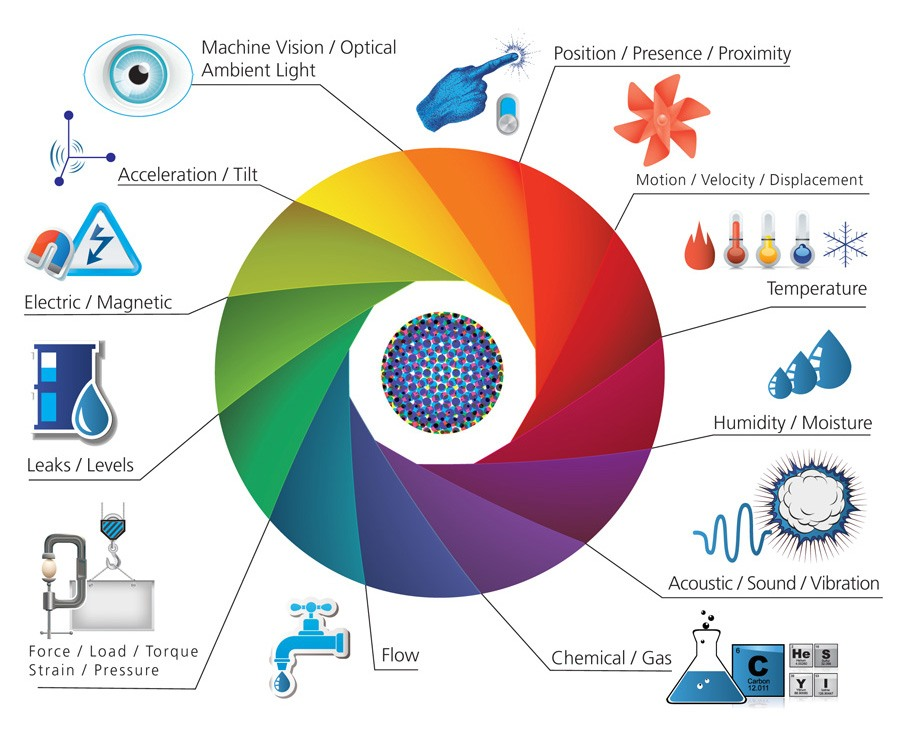
\includegraphics[scale=0.35]{images/sensors.jpg}
\caption{Sensortypen\cite{SensorImage}}
\end{figure}

\subsection{Temperature}%DONE
Temperatursensoren werden in vielen Gebieten eingesetzt. Häufig wird dieser Sensortyp zur Überwachung von Gebäuden eingesetzt, oder hilft bei maschinell hergestellten Esswaren, die richtige Temperatur zu halten. Auch kann ein Bauer diese Sensoren verwenden, um die Bodentemperatur zu Überwachen. So kann man effizienter und gewinnbringender Arbeiten, ohne selber Messungen durchzuführen.
\subsubsection{Bespielgeräte}
\begin{itemize}
\item	Smarte Heizungsteuerungen in einem Haushalt
\item	Wetterstationen
\end{itemize}


\subsection{Acceleration/Tilt}%DONE
Beschleunigungs- und Lagesensoren hat wohl jeder in seiner Hosentasche. Nahezu alle neuen Smartphones haben solche eingebaut. Auch in der Autoindustrie findet man solche sehr häufig. Durch solche Sensoren kann man viele Verschiedene Daten erhalten. So kann man zum Beispiel Bewegungsprofile einer Person erstellen und den Fitnesslevel bestimmen.
\subsubsection{Bespielgeräte}
\begin{itemize}
\item	Schrittzähler (z.B in Smart Watches)
\end{itemize}


\subsection{Acoustic/Sound/Vibration}%DONE
Nicht nur in der Musikbranche sind Akustik- und Soundsensoren sehr wichtig. So wird auch der Lärm in einem Gebiet oder in einer Stadt gemessen, um Verbesserungen der Lebensqualität zu erreichen. Sehr wichtig sind auch die Vibrationssensoren, welche wichtige Daten zu Unterwassererdbeben senden. So können Tsunamis immer früher erkannt werden und retten Leben.
\subsubsection{Bespielgeräte}
\begin{itemize}
\item	Erdbebenwarnsysteme
\item	Sprachsteuerungen
\end{itemize}


\subsection{Chemical/Gas}%DONE
Chemikaliensensoren werden häufig in den Städten mit viel Verkehrsaufkommen eingesetzt. Dadurch wird die Luftqualität bestimmt. Auch in Laboren ist dies ein wichtiger Sensor, um die Qualität oder Reinheit von Gasen zu messen.
\subsubsection{Bespielgeräte}
\begin{itemize}
\item	Smart City Luftüberwachung
\item	Überwachung von gasbetriebenen Geräten
\end{itemize}


\subsection{Electric/Magnetic}
Magnetische Sensoren könnten in verschiedenen Geräten verbaut werden. Zum Beispiel smarte Türschlösser könnten via solchen Sensoren geschlossen oder geöffnet werden. Auch Elektrizitätswerke können diverser solche Sensoren verwenden, um die Systeme zu überwachen.
\subsubsection{Bespielgeräte}
\begin{itemize}
\item	Smarte Schlösser
\item	Stromüberwachung
\end{itemize}


\subsection{Flow}%DONE
Für die Überwachung von Flüssen oder Wasserleitungen werden Flusssensoren verwendet. So können zum Beispiel Wasserversorger den Verbrauch jedes Haushalts über das Internet messen lassen und müssen nicht vor Ort die Zähler ablesen. Oder auch für die Überwachung von Flüssen kann dieser Sensor verwendet werden. So wird man bei zu schnellen und zu vielem Wasser vor Überschwemmungen gewarnt.
\subsubsection{Bespielgeräte}
\begin{itemize}
\item	Smarte Wasserversorgungen
\item	Überschwemmungsschutz
\end{itemize}


\subsection{Force/Load/Torque/Strain/Pressure}%DONE
Im Fitnessbereich gibt es schon seit Jahren mehrere Körperwaagen, welche solche Sensoren verwenden. Man wird gewogen und gleichzeitig sendet das Gerät allerlei Daten an den Cloud-Dienst. Auch Parksysteme oder automatische Wiegesysteme in Lagern sind Beispiele, welche bereits im Einsatz sind. Diese Sensoren sind vielfältig einsetzbar.
\subsubsection{Bespielgeräte}
\begin{itemize}
\item	Wiegesysteme/Körperwaage
\item	Parksysteme
\end{itemize}


\subsection{Humidity/Moisture}%DONE
Ein wichtiger Bestandteil der Luftqualität ist auch die Luftfeuchtigkeit. Diese wird mit diesem Typ gemessen. So können Smart Buildings die Luftfeuchtigkeit laufend messen und immer wieder optimieren. Auch in der Landwirtschaft kann so eine Automation eingeführt werden, damit die Erde immer optimal bewässert ist.
\subsubsection{Bespielgeräte}
\begin{itemize}
\item	Bewässerungsanlagen
\item	Pflanzensensoren
\end{itemize}


\subsection{Leaks/Levels}%DONE
Lecks- und Levelsensoren sind zum Beispiel in der Landwirtschaft notwendig. Die Landwirtschaft benötigt  viel Wasser und man möchte unnötige Lecks vermeiden. Ein weiterer wichtiger Einsatzbereich ist die Überwachung von Flüssigkeitsständen, zum Beispiel bei Staudämmen oder in Lagersystemen.\\
\subsubsection{Bespielgeräte}
\begin{itemize}
\item	Leitungsüberwachungen
\item	Lagerverwaltungen
\end{itemize}


\subsection{Machine Vision / Optical Ambient Light}%DONE
Machine Vision ist ein immer wichtig werdender Sensor. Durch diese kann man den Dingen das Sehen ''lehren''. So sind automatische Eintrittkontrollen möglich. Auch in den SmartCars kommen diese Sensoren zum Einsatz. Da werden durch die Sensoren die Fussgänger, die Fahrbahn oder auch andere Autos erkannt. Bei Optical Ambient Light geht es um Sensoren, welche die Umgebungsbeleuchtung messen und diese Optimal anpassen. So gibt es schon mehrere smarte Leuchtmittel, welche so über das Internet eingestellt werden können.
\subsubsection{Bespielgeräte}
\begin{itemize}
\item	SmartCars
\item	Eintrittskontrollen
\end{itemize}


\subsection{Motion/Velocity/Displacement}%DONE
Bewegungsensoren sind praktische Helfer bei Sicherheitssystemen. Eine zentrale Überwachung von mehreren Gebäuden ist so problemlos möglich. Bei der Pflege von Rollstuhlfahrer wäre zum Beispiel auch eine Falldetektion möglich. Das zentrale Pflegezentrum hätte so eine schnelle Meldung über Unfälle und könnte mehrere Personen überwachen und betreuen.
\subsubsection{Bespielgeräte}
\begin{itemize}
\item	Sicherheitsanlagen
\item	Verkehrsüberwachung
\end{itemize}


\subsection{Position/Presence/Proximity}%DONE
Immer wichtiger wird auch dieser Typ von Sensoren. Durch die Bestimmung von Distanzen oder der Position in einem Raum, ergeben sich viele Einsatzmöglichkeiten. Ein bekanntes Beispiel ist der Abstandssensor bei Autos, um Parkschäden oder Auffahrunfälle zu vermeiden. Oder auch die Gebäudeüberwachung profitiert durch solche Sensoren, da man mehrere Gebäude zentral Überwachen kann.
\subsubsection{Bespielgeräte}
\begin{itemize}
\item	Smarte Parkhäuse
\item	SmartCars
\end{itemize}


\section{Kommunikation}
Internet of Things verbindet Objekte aus der realen Welt miteinander. Um Objekte aus der Realität in die virtuelle Welt zu transformieren, werden Sensoren verwendet. Es gilt nun, diese Sensoren mit dem Internet zu verbinden.

Um unterschiedliche Bedürfnisse abzudecken, sind verschiedene Arten der Kommunikation entstanden. Die mit Sensoren ausgestatteten Geräte können sich in ihrer Weise, mit dem Internet zu kommunizieren stark unterscheiden.

\subsection{Modelle}
\subsubsection{Device-to-Device}
Beim Device-to-Device Kommunikationsmodell kommunizieren mehrere Teilnehmer direkt miteinander (Peer-to-Peer). In diesem Szenario kommunizieren unterschiedliche Glühbirnen drahtlos mit einem Lichtschalter. Kommunikation mit dem Internet ist nicht zwingend notwendig. Eine grosse Herausforderung besteht darin, dass mehrere Teilnehmer unterschiedlicher Hersteller miteinander interagieren können. Dazu müssen die Teilnehmer denselben Protokoll-Stack implementieren. 
\begin{figure}[H]
\centering
\includegraphics[scale=0.8]{images/device-to-device.png}
\caption{Device-to-Device Kommunikation}
\end{figure}
\subsubsection{Device-to-Cloud}
Die Gerätehersteller bieten für ihre End-User Cloud-Dienste im Internet an. Die Sensorgeräte kommunizieren direkt End-to-End über TCP/IP mit dem jeweiligen Cloud-Dienst. Die Benutzer können über eine Mobile App oder eine Webseite auf die jeweiligen Sensordaten zugreifen. Häufig wird aufgrund proprietärer Kommunikationsprotokolle ein Vendor-lock-in betrieben. Dies erschwert die Interoperabilität von Sensoren unterschiedlicher Hersteller \caption{RoseEldridgeChapin15}.
\begin{figure}[H]
\centering
\includegraphics[scale=0.8]{images/device-to-cloud.png}
\caption{Device-to-Cloud Kommunikation}
\end{figure}
\subsubsection{Device-to-Gateway}
\begin{figure}[H]
\centering
\includegraphics[scale=0.8]{images/device-to-gateway.png}
\caption{Device-to-Gateway Kommunikation}
\end{figure}
\subsubsection{Back-End Data-Sharing}
\begin{figure}[H]
\centering
\includegraphics[scale=0.8]{images/backend-data-sharing.png}
\caption{Backend-Data-Sharing Kommunikation}
\end{figure}
\subsection{Architektur}
Man könnte ein IoT System in vier wichtige Gruppen unterteilen: [micrium]
\begin{itemize}
\item Dinge (things)
\item das lokale Netzwerk
\item das Internet
\item Back-End Services (z.B. Cloud Services)
\end{itemize}
\begin{figure}[H]
\centering
\includegraphics[scale=0.8]{images/iot_system_overview_by_micrium.PNG}
\caption{IoT Systemübersicht\cite{IoTOverview}}
\end{figure}
Grundsätzlich scheint die Architektur vertraut. Smart Objects kommunizieren über ein lokales Netzwerk mit Diensten im Internet.

Bisher konnten Geräte wie Laptops, PCs und Smartphones beinahe einheitlich mit dem Internet verbunden werden; entweder verkabelt über Ethernet oder drahtlos über ein lokales WLAN oder mobile Netze wie UMTS und LTE. Die Endgeräte verfügten jeweils über viel Rechenleistung, Speicher und ein leistungsfähiges Betriebssystem mit einem vollständig implementierten TCP/IP Stack. 

In einem IoT System muss man von einer grossen Anzahl an Geräten mit Sensoren ausgehen. Diese Geräte verfügen meist über eine extrem niedrige Bandbreite, wenig Speicher und Rechenleistung [youtube].
\subsection{Wireless Sensor Netzwerke}
Bei einer Vielzahl von verbundenen Sensoren, welche über einen grossen Bereich verstreut sind, bietet sich ein Wireless Sensor Network (WSN) an. In einem WSN werden die Sensoren nicht direkt mit dem Internet verbunden. Die Daten werden drahtlos von Teilnehmer zu Teilnehmer versendet. Muss ein Datenpaket in ein entferntes Netzwerk wie das Internet, so wird ein Gateway oder Edge Node benötigt.
\begin{figure}[H]
\centering
\includegraphics[scale=0.8]{images/iot_wsn_lan_overview_by_micrium.PNG}
\caption{IoT WSN\cite{IoTWSN}}
\end{figure}
WSN Nodes sind typischerweise günstig im Einkauf. Sie können mit sehr wenig Leistung betrieben werden, dies ermöglicht den Batteriebetrieb. Durch diese Eigenschaften können WSN Nodes einfach, schnell und in sehr grosser Anzahl bereitgestellt werden. 
\chapter{IoT Device Management}
In Zukunft ist eine stark ansteigende Anzahl an IoT Devices zu erwarten. 
\section{Device Management Kategorien}
FCAPS blabla
\subsection{Provisionierung und Authentisierung}
\subsection{Konfiguration}
\subsection{Monitoring und Diagnose}
Ein wichtiger Teil des IoT Management ist das Monitoring und die Diagnose. 


Wieso
wichtiger teil, zentral verfügbar, 





Proactive problem detection 
Helps decrease time for troubleshooting and diagnosis 
maximize system uptime and improve productivity

Logging

Überwachung -> Compute, storage, networking
Nicht 100\% benötigt

Zentral

Security



\subsection{Maintenance und Update}






\subsection{Security Management}



\section{}





















\chapter{Kommunikation}
\section{Architektur}
Man könnte ein IoT System in vier wichtige Gruppen unterteilen: \cite{IoTNetworks}
\begin{itemize}
\item Dinge (things)
\item das lokale Netzwerk
\item das Internet
\item Back-End Services (z.B. Cloud Services)
\end{itemize}
\begin{figure}[H]
\centering
\includegraphics[scale=0.8]{../02_Analyse/images/iot_system_overview_by_micrium.png}
\caption{IoT Systemübersicht\cite{IoTOverview}}
\end{figure}
Grundsätzlich scheint die Architektur vertraut. Smart Objects kommunizieren über ein lokales Netzwerk mit Diensten im Internet.

Bisher konnten Geräte wie Laptops, PCs und Smartphones beinahe einheitlich mit dem Internet verbunden werden; entweder verkabelt über Ethernet oder drahtlos über ein lokales WLAN oder mobile Netze wie UMTS und LTE. Die Endgeräte verfügten jeweils über viel Rechenleistung, Speicher und ein leistungsfähiges Betriebssystem mit einem vollständig implementierten TCP/IP Stack. 

In einem IoT System muss man von einer grossen Anzahl an Geräten mit Sensoren ausgehen. Manchmal verfügen diese Geräte über eine extrem niedrige Bandbreite, wenig Speicher und Rechenleistung \cite{CiscoIoTArchitecture}.

Die Kommunikation erfolgt oft nicht vertikal der Architektur, sondern auch horizontal auf derselben Ebene. Sensordevices können beispielsweise miteinander kommunizieren oder Cloud Services Daten der Sensoren untereinander austauschen.
\subsection{Wireless Sensor Netzwerke}
Bei einer Vielzahl von verbundenen Sensoren, welche über einen grossen Bereich verstreut sind, bietet sich ein Wireless Sensor Network (WSN) an. In einem WSN werden die Sensoren nicht direkt mit dem Internet verbunden. Die Daten werden drahtlos von Teilnehmer zu Teilnehmer versendet. Muss ein Datenpaket in ein entferntes Netzwerk wie das Internet, so wird ein Gateway oder Edge Node benötigt.
\begin{figure}[H]
\centering
\includegraphics[scale=0.8]{../02_Analyse/images/iot_wsn_lan_overview_by_micrium.png}
\caption{IoT WSN\cite{IoTWSN}}
\end{figure}
WSN Nodes sind typischerweise günstig im Einkauf. Sie können mit sehr wenig Leistung betrieben werden, dies ermöglicht den Batteriebetrieb. Durch diese Eigenschaften können WSN Nodes einfach, schnell und in sehr grosser Anzahl bereitgestellt werden. 

\section{Kommunikationsmodelle}
Internet of Things verbindet Objekte aus der realen Welt miteinander. Um Objekte aus der Realität in die virtuelle Welt zu transformieren, werden Sensoren verwendet. Es gilt nun, diese Sensoren mit dem Internet zu verbinden.

Um unterschiedliche Bedürfnisse abzudecken, sind verschiedene Arten der Kommunikation entstanden. Die mit Sensoren ausgestatteten Geräte können sich in ihrer Weise, mit dem Internet zu kommunizieren stark unterscheiden.

\subsection{Device-to-Device}
Beim Device-to-Device Kommunikationsmodell kommunizieren mehrere Teilnehmer direkt miteinander (Peer-to-Peer). In diesem Szenario kommunizieren unterschiedliche Glühbirnen drahtlos mit einem Lichtschalter. Denkbar wären sämtliche Anwendungsgebiete aus dem \glqq Smart Home\grqq -Bereich. Kommunikation mit dem Internet ist nicht zwingend notwendig. Eine grosse Herausforderung besteht darin, dass mehrere Teilnehmer unterschiedlicher Hersteller miteinander interagieren können. Dazu müssen die Teilnehmer denselben Protokoll-Stack implementieren. 
\begin{figure}[H]
\centering
\includegraphics[scale=0.8]{../02_Analyse/images/device-to-device.png}
\caption{Device-to-Device Kommunikation}
\end{figure}
\subsection{Device-to-Cloud}
Die Gerätehersteller bieten für ihre End-User Cloud-Dienste im Internet an. Die Sensorgeräte kommunizieren direkt End-to-End über TCP/IP mit dem jeweiligen Cloud-Dienst. Die Benutzer können über eine Mobile App oder eine Webseite auf die jeweiligen Sensordaten zugreifen. Häufig wird aufgrund proprietärer Kommunikationsprotokolle ein Vendor-lock-in betrieben. Dies erschwert die Interoperabilität von Sensoren unterschiedlicher Hersteller \cite{RoseEldridgeChapin15}.
\begin{figure}[H]
\centering
\includegraphics[scale=0.8]{../02_Analyse/images/device-to-cloud.png}
\caption{Device-to-Cloud Kommunikation}
\end{figure}
\subsection{Device-to-Gateway}
Anstatt einer Ende-zu-Ende Kommunikation zwischen Sensoren und Servern wird in diesem Modell ein Gateway zwischen diesen Komponenten eingesetzt. Sensoren kommunizieren somit nicht direkt mit einem Server. Auf diese Art und Weise können eine grosse Anzahl Sensoren mit Internetdiensten verbunden werden ohne dass die Sensoren selbst über einen direkten Internetzugriff verfügen. Der Gateway muss somit über eine Schnittstelle verfügen, damit Dienste im Internet indirekt mit den Sensoren kommunizieren können. Aus Sicht des Diensts ist es irrelevant, wie der Gateway mit den Sensoren kommuniziert.
\begin{figure}[H]
\centering
\includegraphics[scale=0.8]{../02_Analyse/images/device-to-gateway.png}
\caption{Device-to-Gateway Kommunikation}
\end{figure}
\subsection{Back-End Data-Sharing}
Sobald sich die Sensordaten auf einem Server befinden, können diese auf bekannte Weise anderen zur Verfügung gestellt werden. Beispielsweise könnte man den Zustand eines Sensors als JSON Objekt über eine REST-Schnittstelle abfragen. Ein weiterer Serviceprovider muss somit nicht mehr direkt mit den Sensoren kommunizieren. Da Sensordevices oft über limitierte Möglichkeiten verfügen, grössere Datenmengen bereitzustellen, verringert man mit dieser Art der Kommunikation die Anzahl Abfragen auf den Sensordevices. 
\begin{figure}[H]
\centering
\includegraphics[scale=0.8]{../02_Analyse/images/backend-data-sharing.png}
\caption{Backend-Data-Sharing Kommunikation}
\end{figure}

\newpage

\section{IoT Kommunikationsprotokolle}
Seit der Entstehung des Internets werden für unterschiedliche Aufgaben Kommunikationsprotokolle entwickelt. Eine grosse Herausforderung war stets die Interoperabilität zwischen Geräten unterschiedlicher Hersteller. Standardisierungsgremien wie die International Standards Organization (ISO) und die Internet Engineering Task Force (IETF) haben in den vergangenen Jahrzehnten Richtlinien und Standardisierung von Kommunikationsprotokollen veröffentlicht. 

Mit zunehmender Popularität des Internets der Dinge sind eine unüberschaubare Menge an proprietären und offenen Kommunikationsprotokollen entstanden. In der Geschichte des Internets hat sich gezeigt, dass sich langfristig nur offene Protokolle durchsetzen werden \cite{Obermaier14}, proprietäre Protokolle hingegen werden aufgrund der fehlenden Interoperabilität niemals eine breite Verwendung finden.
\subsection{Anforderungen}
Bereits heute zeichnen sich die populärsten IoT Kommunikationsprotokolle ab. Um zu verstehen weshalb-, und vor allem in welchen Szenarien welches Protokoll eingesetzt wird respektive werden sollte, muss man sich mit den unterschiedlichen Anforderungen vertraut machen.

Die typischen bekannten Fragen nach der Verbreitung/Unterstützung und Skalierbarkeit stellen sich auch hier. Ebenfalls muss auf die mutmassliche Datenmenge geachtet werden. So dürfte eine vergleichsweise hohe Datenmenge für Geräte, welche über einen direkten, verkabelten Internetzugang verfügen, kein Problem darstellen, während Geräte in einem Mesh-betriebenen WSN wohl über deutlich weniger Bandbreite verfügen dürften.

Weitere Anforderungen wären Realtime Kommunikation, Stromverbrauch, Sicherheit und Network Address Translation (NAT) \cite{Obermaier15}.
\subsection{Request/Response}
Request/Response ist das wohl bekannteste Pattern. Ein Client fordert mittels eines Requests eine Response von einem Service an. Der Service hört auf einkommende Requests, verarbeitet diese und antwortet (Response) den aufrufenden Clients. Request/Response Kommunikation skaliert schlecht, deshalb sollte beim Versenden einer Meldung an viele Teilnehmer auf ein anderes Pattern zurückgegriffen werden. 
\begin{figure}[H]
\centering
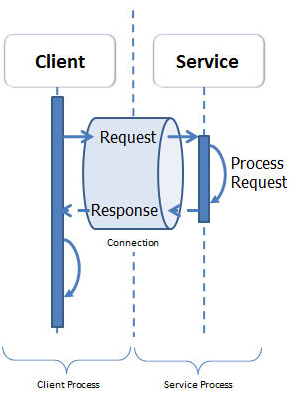
\includegraphics[scale=0.8]{../02_Analyse/images/request-response.png}
\caption{Request/Response Kommunikation \cite{ReqRes}}
\end{figure}
\subsubsection{HTTP}
In den 1990er Jahren wurde HTTP verwendet um statische HTML-Dokumente übers Internet abzurufen. Bis heute hat sich die grundsätzliche Funktion von HTTP nicht verändert. HTTP bietet über seine Methoden ein umfangreiches Interface für die Request/Response Kommunikation zwischen Clients und Servern über das Internet. 

Aufgrund seiner hohen Verbreitung, Standardisierung und Unterstützung ist HTTP auch im IoT Umfeld beliebt. Für fast jede Programmiersprache und Laufzeitumgebung existieren Libraries, was das Entwickeln sehr angenehm macht. HTTP eignet sich jedoch nicht für alle Anwendungsfälle im IoT Bereich. Für jeden Request wird der gesamte HTTP (und darunterliegende) Header benötigt. Zusätzlich ist das Protokoll textbasiert, was mit dem zusätzlichen, grossen Overhead eine erhebliche Datenmenge bedeuten könnte. Für Endgeräte an Mobilen Netzwerken könnte dies ungeeignet sein \cite{Obermaier15}.

In der Version 1, respektive 1.1 gibt es mit HTTP keine Möglichkeit, echte Push-Meldungen zu versenden. Bei Push-Meldungen sendet der Server eine Response (besser: Nachricht) an den Client ohne vorgängigen Request. In der Version 2 von HTTP sind echte Push-Meldungen vorgesehen, jedoch gibt es wenige Implementation und Erfahrungswerte damit.
\subsubsection{CoAP}
Das Constrained Application Protocol (CoAP) implementiert wie HTTP das Request/Response Pattern \cite{Obermaier15}. Mit CoAP existiert ein massgeschneidertes IoT-Protokoll, welches nach dem REST Paradigma konzipiert wurde. HTTP ist schwergewichtig, hat einen grossen Overhead und generiert damit hohe Datenmengen. Ausserdem ist vor jeder Session den für TCP benötigten 3-Way Handshake nötig. 
 
CoAP wurde entwickelt, um diesen Schwächen von HTTP entgegenzuwirken. Bei sogenannten Low-Power and Lossy Networks (LLN's) sind die Nodes im Vergleich zu herkömmlichen Computersystemen sehr eingeschränkt, was die Verwendung von HTTP schwierig gestaltet. CoAP bietet grundsätzlich folgende Features:\cite{RFC7252}
\begin{itemize}
\item Request/Response Kommunikation zwischen Endpoints	
\item Discovery von Services und Ressourcen
\item URI's und Media Types
\item Kompatibilität mit HTTP
\item Multicast Support
\item sehr kleiner Overhead (Header von 4 Byte)
\item implementiert das Observer Design Pattern
\item UDP als Transportprotokoll
\item Asynchroner Nachrichtenaustausch
\end{itemize}
 
CoAP kann Peer-to-Peer zwischen Devices eingesetzt werden, aber auch zwischen Device und Service oder zwischen Device und einem Proxy.
\begin{figure}[H]
\centering
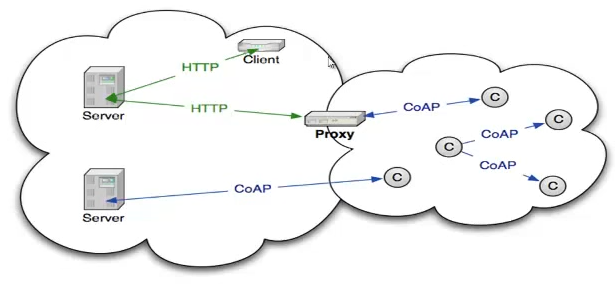
\includegraphics[scale=0.8]{../02_Analyse/images/coap_architecture.png}
\caption{CoAP Architektur \cite{Shelby14}}
\end{figure}
  
Durch die massgeschneiderten Features für IoT wird CoAP hauptsächlich in WSN's eingesetzt \cite{Obermaier15}. 

\subsection{Publish/Subscribe}
Beim Publish/Subscribe Pattern gibt es einen Sender (Publisher) und einen Empfänger (Subscriber). Der Empfänger hört auf gewisse Themen (Topics). Dies kann nur ein Thema sein oder auch viele Verschiedene. Der Sender kategorisiert seine Nachrichten in Themen und sendet diese zu den jeweiligen Empfänger. Der Sender und der Empfänger wissen aber nichts voneinander. Sie senden oder hören nur im Netzwerk, ob eine für sie interessante Nachricht angekommen ist. Durch die einfache Verknüpfung von Publisher und Subscriber, eignet sich dieses Verfahren sehr gut im IoT-Bereich. Die Sensoren sind die Publisher, sie liefern zum Beispiel Temperaturdaten in die richtige Kategorie. Alle Server/Clouddienste, welche sich für Temperaturdaten interessieren, können auf diese Kategorie hören. Durch die einfache Handhabung skaliert dieses Pattern sehr gut.

In der folgenden Grafik sieht man das Publish and Subscribe Pattern. Der Publisher hat eine ''Address Changed'' Message in den Channel geschickt. Nun erhalten alle Subscriber, welche dem Channel folgen, diese Nachricht und verarbeiten sie.

\begin{figure}[H]
\centering
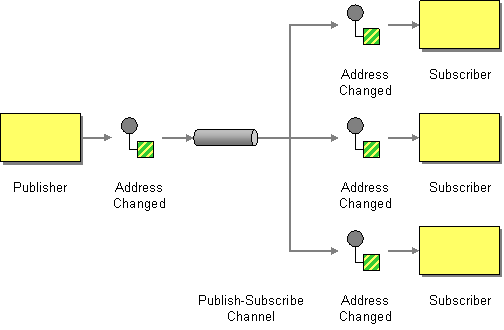
\includegraphics[scale=0.65]{../02_Analyse/images/publishsubscribe.png}
\caption{Publish and Subscribe Pattern\cite{PublishSubscribePattern}}
\end{figure}
\subsubsection{MQTT}
MQTT (Message Queue Telemetry Transport) ist ein von IBM entwickeltes Protokoll. Es ist ein speziell für IoT entwickeltes Protokoll um Machine-to-Machine Kommunikation herzustellen. Bei dem Protokoll wurde speziell auch ein schlankes Design geachtet. So ist die kleinst mögliche Nachricht gerade mal 2 Byte gross. 

Der Hauptverwendungszweck von MQTT ist vor allem der Austausch von Daten zwischen Geräten und Server (D2S).\cite{ProtPubSub} Da das Protokoll für die D2D Konnektivität entwickelt wurde, wird es auch in diesem Bereich eingesetzt. Das heisst die Vorteile liegen in Netzen mit vielen kleinen Geräten, welche wenig Kommunizieren und sich als Kollektion sehen.\cite{ProtPubSubReason}

Bei MQTT wird ein Broker verwendet. Der Sensor ''published'' seine Daten mit einem Topic und den Daten an den Broker. Dieser sendet die Nachricht an alle, welche sich auf das gewünschte Topic Subscribed haben. Durch das schlanke Design, gibt es natürlich auch Nachteile. Aber bei kleinen und einfachen Systemen ist MQTT ein beliebtes Protokoll.
\subsubsection{AMQP}
AMQP (Advanced Message Queuing Protocol) ist ein bekanntes und viel eingesetztes Protokoll. Das binäre Netzwerkprotokoll wird von vielen grossen Firmen\cite{ProtPubSubReason} entwickelt, wie zum Beispiel Microsoft oder auch Cisco. Momentan ist die Version 1.0 seit 2010 als aktuellen Standard im Einsatz.

AMQP wird durch sein Queuing Design im Server zu Server Bereich eingesetzt (S2S).\cite{ProtPubSub} Daher ist es in Bereichen einzusetzen, in der die Geschwindigkeit und der Prozessor nicht relevant sind. Zusätzlich wird es in Bereichen eingesetzt, in dem eine Nachricht nur von A nach B gesendet werden soll und man keine Nachricht verlieren möchte.

Die Sensoren senden die Nachrichten an einen Message Broker, welcher die Nachricht in die richtige Queue schiebt. Nun können sich die Dienste an der Queue anmelden und die Nachrichten konsumieren. Dabei gibt es die Möglichkeit Topics zu setzen, um Kategorien einzuführen. Es können jeder Nachricht auch noch Attribute hinzugefügt werden, wie zum Beispiel Name oder Durability. Durch den grossen Funktionsumfang des Protokolls ist es natürlich auch schwieriger einzurichten und die minimale Paketgrösse wächst damit auch. Die kleinstmögliche Paketgrösse ist 60 Byte.
\subsubsection{XMPP}
XMPP (Extensible Messaging and Presence Protocol) wurde speziell für das Internet der Dinge erweitert, um den Anforderungen gerecht zu werden. XMPP gibt es schon seit mehreren Jahren und wurde in vielen Chatprogrammen eingesetzt. Auch heute findet man das Protokoll beim Facebook-Messenger wieder. Mit der IoT-Erweiterung/Anpassung will man nun nicht mehr Menschen miteinander verknüpfen, sondern Dinge. 

XMPP ist das beste Protokoll um Geräte mit Menschen zu verbinden. Dies ist eine Spezialform des Geräte zu Server Pattern (D2S). \cite{ProtPubSub} XMPP sollte dann verwendet werden, wenn die Geschwindigkeit und der Prozessor nicht wichtig sind, wenn das Gerät immer verbunden sein soll und wenn nur wenige Konnektivitätspunke in einem grossen Bereich vorhanden sind.\cite{ProtPubSubReason}

Bei XMPP wird kein Broker, sondern ein zentraler Server verwendet. Dieser soll allerlei verschiedene Geräte miteinander verbinden. Dieses Protokoll wird häufig für das Remote Management von Konsumergeräten verwendet.

\newpage

\section{LwM2M - Lightweight M2M}
\subsection{Einführung}
LwM2M ist ein speziell für IoT entwickeltes Management- und Messaging-Protokoll. Wie es der Name schon verrät, handelt es sich um ein M2M - Machine-to-Machine Protokoll. Bei LwM2M wird ein Client-Server-Modell umgesetzt. Dabei werden alle Daten per Request angefragt und als Response beantwortet.

Entwickelt und standardisiert wurde dieses durch die Open Mobile Alliance, kurz OMA. Die Oma ist ein Verbund aus Firmen, welche in der Mobilfunksparte tätig sind, wie zum Beispiel Nokia, Motorola oder auch viele grosse Mobilfunkprovider. 

\subsection{Protocol Stack}

LwM2m ist ein Applikationslayer Protokoll und hat als Basis das CoAP Protokoll. Alle LwM2M Befehle werden umgewandelt, damit diese über CoAP zum Geräte gesendet werden. Dabei werden nicht alle Features von CoAP eingesetzt und unterstützt. CoAP ist wie auch LwM2M speziell für M2M (Maschine-to-Machine) Applikationen entwickelt worden.

Unterhalb von CoAP gibt es drei Varianten, die am gebräuchlichsten sind. UDP, UDP mit DTLS und SMS. Verwendet man nur UDP wird keine Verschlüsselung verwendet. Alle Daten werden in Klartext übertragen. Um eine sichere Verbindung herzustellen muss DTLS eingerichtet werden. Zusätzlich gibt es noch die Möglichkeit SMS. Diese ist speziell für Geräte ohne Internetanschluss gedacht. Alle Anfragen werden in ein SMS gepackt und so über das Telekommunikationsnetz übertragen.

Unterhalb der Verbindungsschicht können wieder viele verschiedene Technologien eingesetzt werden. Dies ist unter anderem IPv4, IPv6, 6LoWPAN oder auch ZigBee IP. 

Mit all diesen Möglichkeiten bietet LwM2M eine grosse Abdeckung an Technologien und kann vielseitig eingesetzt werden. 
\begin{figure}[H]
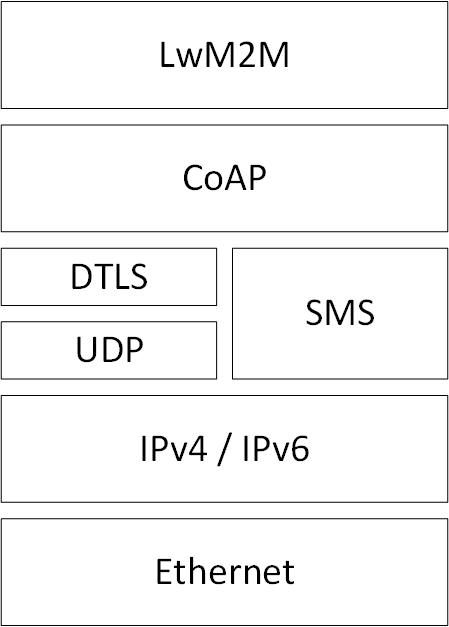
\includegraphics[scale=0.3]{../02_Analyse/images/lwm2m/stack.png}
\caption{LwM2M Stack}
\end{figure}

\newpage

\subsection{Client-Server Model}
\begin{figure}[H]
\includegraphics[scale=0.5]{images/lwm2m/server_client_model.png}
\caption{Client-Server-Model}
\end{figure}
Die drei zentralen Bestandteil des Protokolls sind der Bootstrap-Server, der LwM2M-Server und der LwM2M-Client. Der Bootstrap-Server ist für den Erstkontakt sowie die Erstkonfiguration zuständig. Die restliche Kommunikation läuft zwischen dem LwM2M-Server und dem LwM2M-Client. Ohne einen Bootstrap-Server kommunizieren die Geräte direkt mit dem LwM2M-Server.
\subsubsection{Client}
Der Client kann viele verschiedene Formen annehmen. Ein Beispiel wäre eine Linux Installation auf einem Raspberry Pi, welche einen Java LwM2M Client gestartet hat. An dem Raspberry Pi kann man nun mehrere Sensoren, wie Temperatur, Druck, etc. anschliessen und diese über den Client steuern. Es kann sich aber auch nur um einen kleinen Chip mit Sensor handeln, welcher ein C LwM2M Client beinhaltet. Client Umsetzungen gibt es dabei in den Programmiersprachen C und Java.
\subsubsection{Server}
Die Serverumsetzung ist sehr ähnlich wie die Clientumsetzung. Es wird auf einem Server eine Serverinstanz gestartet und diese wartet auf Clients, welche sich Registrieren möchten. Da die Serverimplementierung, wie auch der Client in C und Java verfügbar ist, gibt es viele Möglichkeiten den Server zu deployen. So kann er auf einer Windows- sowie auch unter Linux gestartet werden. Der Server hört dann auf dem CoAP Port auf die Anfragen.
\subsubsection{Management Server}
Der Management Server klinkt sich nun beim LwM2M Server ein. Dieser Server kann direkt oder über ein Web API angesprochen werden. Je nach Implementierung gibt es beide Varianten. So könnte man mehrere Serverinstanzen zu einem Management Server hinzufügen, um alles zentral Verwalten zu können. Möchte man nun ein Gerät managen, schickt man einen Befehl an den zuständigen LwM2M Server und dieser leitet den Befehl nun an das Device weiter. Die Antwort wird danach bis zum Management Server zurückgegeben und ausgewertet. 
\subsubsection{Bootstrap-Server}
Um ein ''factory bootstrap'' zu vermeiden, hat LwM2M einen Bootstrap-Server. Dieser ist für die Erstkonfiguration Zuständig und macht die Geräte variabler einsetzbar. Auf der Grafik ist dieser nicht erfasst worden. Wichtige Einstellungen die der Bootstrap-Server verteilen kann sind unter anderen\cite{BootstrapFeatures}:
\begin{itemize}
\item Keys  und Zertifikate für DTLS
\item Server URL
\item SMS Security Parameter
\item Kommunikationsparameter
\item Access Control Lists
\end{itemize}
Durch den Einsatz von Bootstraping nimmt man sich viel Managementarbeit ab und hat ein einheitlicheres und besser verwaltetes Netzwerk von LwM2M-Server und Client.
\begin{figure}[H]
\includegraphics[scale=0.5]{../02_Analyse/images/lwm2m/server_client_model.png}
\caption{Client-Server-Model}
\end{figure}
\subsection{Object Model}
Eine klare Stärke des LwM2M-Protokolls sind die Object Models. Durch die Object Models werden alle Informationen eines Devices in einem strukturierten Model abgelegt, damit ein geregelter Zugriff auf alle Daten entsteht. Es wird zwischen Object, Instance und Ressource unterschieden. Eine Ressource ist zum Beispiel der Temperaturwert eines Temperatursensors. Eine zusätzliche Ressource könnte die dazugehörige Temperatureinheit sein. Mehrere solche Ressourcen werden zu einem Object Model zusammengefasst. Ein Device kann aber auch mehrere Temperatursensoren besitzen und hat so mehrere Instanzen des gleichen Objects.

Um nun die Information zugreifbar zu machen, bekommt sie eine URL mit den drei oben beschriebenen angaben. Diese kann wie folgt aussehen.
%TODO Bild einfügen
\begin{figure}[H]
%\includegraphics[scale=0.5]{}
\caption{Object Model URL}
\end{figure}
\subsubsection{Aufbau}
\subsubsection{Object}
Jedes Object besitzt eine eindeutige Identifikationsnummer. Diese geht von 0-32768 und ist folgendermassen verteilt:
\begin{itemize}
\item 0-1023: OMA-Label
\item 1024-2047: Reserviert für zukünftige Benutzung
\item 2048-10240: Registrierungen der Partnerfirmen
\item 10241-32768: Individuelle Registrierungen durch Firmen oder Personen
\end{itemize}
Wenn man ein neues Model erstellen möchte, geht man auf die OMA-Seite und erfasst dieses im ''LWM2M Management Object Editor''. Pro neuem Modell muss man eine Object ID, Namen, ObjectVersion, LWM2MVersion, Object URN, Instances und Mandatory festlegen. Mit Instances gibt man an, ob ein Object pro Device mehrmals vorhanden sein darf.
\subsubsection{Instances}
Wenn ein Object mehrmals vorhanden sein kann, wie zum Beispiel ein Temperaturobjekt, gibt es die Möglichkeit der Multiinstanz. Der mittlere Teil der URL nimmt dadurch nicht nur den Wert 0 an, sondern eine eindeutige ID pro Instanz.

\subsubsection{Ressource}
Dem Object werden zum Schluss noch die Ressourcen hinzugefügt. Diese besitzen auch eine eindeutige Identifikationsnummer von 0 bis 32768. Hier gibt es folgende Unterteilung:
\begin{itemize}
\item 0-2047: Common Ressources
\item 2048-26240: Reusable Ressources
\item 26241-32768: Private Ressources
\end{itemize}
Jede Ressource hat vordefinierte Felder. Dazu gehören Name, Operations, MultipleInstances, Mandatory, Type, RangeEnumeration, Units und Description. Durch all diese Felder kann eine Ressource sehr genau beschrieben werden. Nicht alle Felder sind Pflicht, aber wichtig sind vorallem ID, Name und Operations und Type. Durch die Operations gibt man an, was mit dieser Ressource genau gemacht werden kann. Hier kann man zwischen Read, Write, Read-Write und Execute wählen.	Mit dem Type Feld gibt man den Type Informationstyp an, wie zum Beispiel String, Float oder Date.


Durch all diese Standardisierten Objekte und Ressourcen kann man jede Information eines Gerätes beschreiben und es entstehen keine Kompatibilitätsprobleme.
\subsubsection{Beispiel XML}
Hier sieht man ein Beispiel von dem Object Model ''Device'' mit der Ressource ''0 - Manufacturer''. Das Object Model besitzt aber noch weitere Ressourcen, die andere Informationen eines Devices definieren.
\begin{lstlisting}[%
language=xml]
<LWM2M>
	<Object">
		<Name>Device</Name>
		<Description1><![CDATA[ This LWM2M Object ... ]]></Description1>
		<ObjectID>3</ObjectID>
		<ObjectURN>TBD</ObjectURN>
		<MultipleInstances>Single</MultipleInstances>
		<Mandatory>Mandatory</Mandatory>
		<Resources>
			<Item ID="0">
				<Name>Manufacturer</Name>
				<Operations>R</Operations>
				<MultipleInstances>Single</MultipleInstances>
				<Mandatory>Optional</Mandatory>
				<Type>String</Type>
				<RangeEnumeration />
				<Units/>
				<Description><![CDATA[ Human rea... ]]</Description>
			</Item>
			<Item>...</Item>
		</Resources>
	</Object>
</LWM2M>
\end{lstlisting}

\subsubsection{Beispiel Client}
Hier sieht man nun ein Beispielclient. Dies könnte eine kleine LED-Lampe sein, welche jedes LED separat steuern lässt. Dazu wurden die Objeke 3 und 3311 verwendet, welche bereits vorgefertigt bereitstehen. Da es mehrere LEDs gibt, werden auch mehrere Light Control Instanzen benötigt. Jede Instanz steuert so eine einzelne LED.
Neben diesen drei Objekten könnten noch weitere vorhanden sein, wie zum Beispiel Firmware oder andere Sensorobjekte.
\begin{figure}[H]
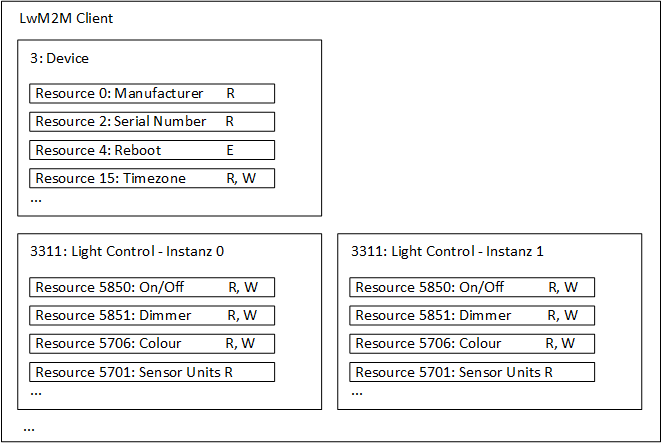
\includegraphics[scale=0.65]{../02_Analyse/images/lwm2m/lwm2m_client.png}
\caption{LwM2M Stack}
\end{figure}

\newpage

\subsection{Features und Funktionen}
LwM2M bietet vier Funktionen, um mit einem Device zu kommunizieren oder diesen zu konfigurieren. Bootstraping, Registration, Object / Ressource Access und Reporting. Es müssen aber nicht immer alle Funktionen eingesetzt werden. So kann auf Bootstraping und Reporting verzichtet werden, wenn man jedes Device von Hand vorkonfiguriert.
\subsubsection{Bootstrapping - Allgemein}
Wie oben bereits erwähnt, ist das ''factory bootstraping'' möglichst zu vermeiden. Durch die statisch hinterlegten Keys und Server-URLs muss man bei jeder Anpassung der Daten physischen Zugriff auf das Device haben. Dies ist ein Ansatz, der vielleicht bei normalen Computern noch funktioniert hat, aber dies funktioniert bei IoT-Geräten selten gut. Daher hat das LwM2M-Protokoll einen Bootstrap-Vorgang definiert.


Der Hersteller muss für das Bootstraping jedem Gerät ein Endpointname, sowie eine Bootstrap-URL hinterlegen. Alle anderen Informationen, werden beim Starten vom Bootstrap-Server geholt.
Wichtige Einstellungen die der Bootstrap-Server verteilen kann sind unter anderen\cite{BootstrapFeatures}:
\begin{itemize}
\item Keys  und Zertifikate für DTLS
\item Server URL
\item SMS Security Parameter
\item Kommunikationsparameter
\item Access Control Lists
\end{itemize}
Durch den Einsatz von Bootstraping nimmt man sich viel Managementarbeit ab und hat ein einheitlicheres und besser verwaltetes Netzwerk von LwM2M-Server und Client.
\subsubsection{Bootstrapping - Ablauf}
Sobald ein Device gestartet wird, überprüft es seine Einstellungen. Es gibt zwei Zeitpunkte, an denen der Device einen Bootstrap-Server kontaktiert. Der erste ist, sobald der Device nur Bootstrap-Server Daten besitzt und keine LwM2M-Server Daten hinterlegt hat. Die zweite Möglichkeit ist, wenn der L2M2M-Server keine Antwort mehr gibt oder Authentifikation fehlgeschlagen meldet. Sobald dies geschieht, meldet sich der Device wieder beim Bootstrap-Server, um eine neue konfiguration zu erhalten.

In der folgenden Grafik sieht man den Ablauf des Bootstrapings.
\begin{figure}[H]
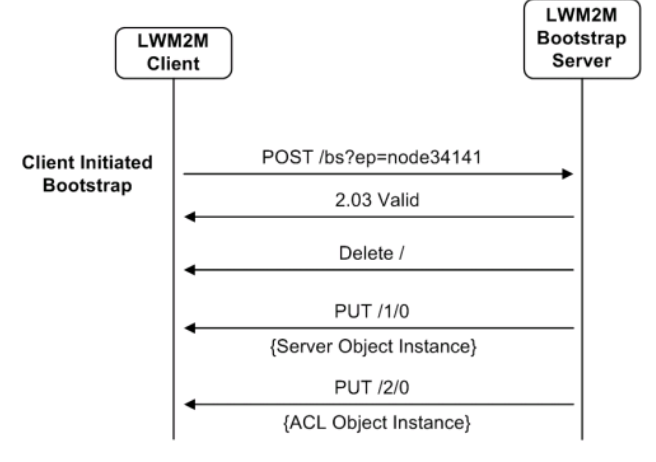
\includegraphics[scale=0.5]{../02_Analyse/images/lwm2m/bootstrap_diagram.png}
\caption{LwM2M Bootstraping\cite{LwM2MInterfaces}}
\end{figure}
Als ersten Schritt sendet der Device eine Anfrage an den Bootstrap-Server. In dieser Anfrage gibt der Client sein Endpointname an. Durch diesen Endpointname weiss der Bootstrap-Server, welche Konfiguration für dieses Gerät vorgesehen ist. Der Server antwortet mit ''Valid''. Durch einen Delete Befehl auf die Root-URL löscht es die alten Konfigurationen. Danach werden durch einzelne PUTs alle wichtigen Daten auf das Gerät geschrieben.

Wenn der Server eine neue Konfiguration, wie zum Beispiel neues Schlüsselmaterial, verteilen möchte, löscht der LwM2M-Server durch einen Delete wieder die Root-URL auf dem Client. Dadurch meldet sich der Client wieder beim Bootstrap-Server, um die neuen Daten zu erhalten. Dies nennt man den  Server imitierte Bootstrap-Vorgang.

\subsubsection{Registration - Allgemein}
Wenn ein Client einen gültigen und erreichbaren LwM2M-Server hinterlegt hat, beginnt die Registrierungsphase. Bei der Registrierung wird dem Server bekanntgeben, welche Funktionen und Informationen der Client besitzt. Dies beinhaltet die Object Model URLs, Registrierungszeitpunkt, IP-Adresse, Port und noch weitere Angaben, die der Server von jedem Client benötigt. All diese Angaben werden vom Client immer wieder aktualisiert und an den Server gesendet. Dies geschieht meistens mehrmals pro Minute.

\subsubsection{Registration - Ablauf}
\begin{figure}[H]
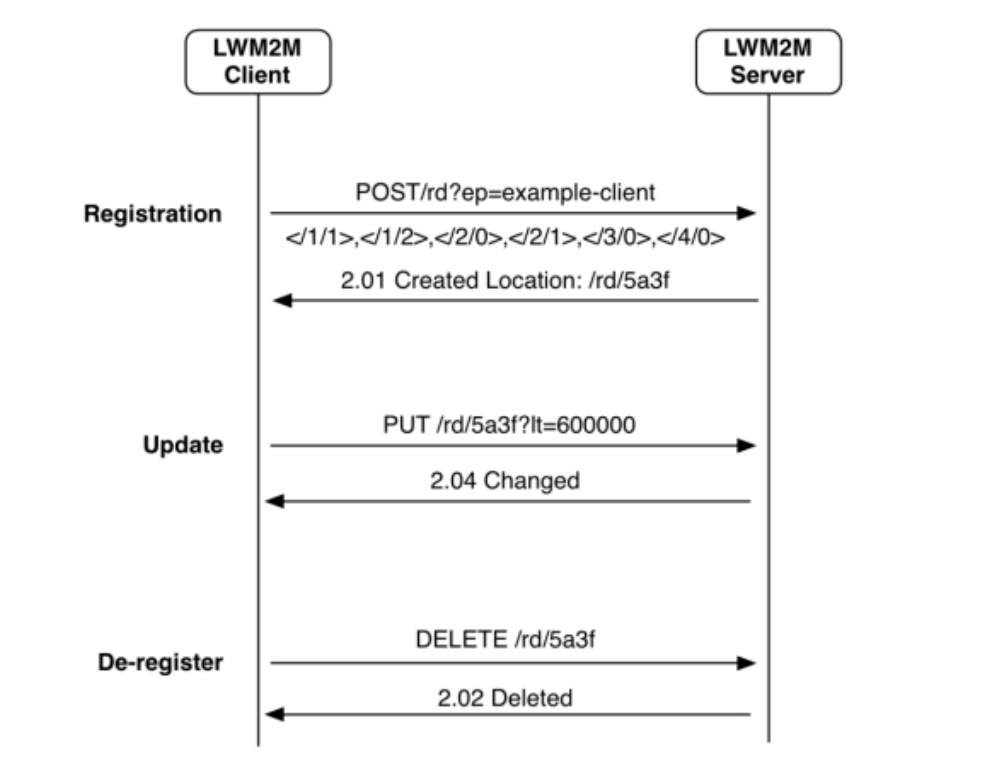
\includegraphics[scale=0.4]{../02_Analyse/images/lwm2m/registration_diagram.png}
\caption{LwM2M Stack\cite{LwM2MInterfaces}}
\end{figure}
Die Registrierung wird immer von einem Client aus gestartet. Dieser sendet seinem hinterlegtem LwM2M-Server einen POST mit all den relevanten Daten. Sobald diese gesendet wurden, wartet der Client auf eine Antwort. Der Server überprüft nun diese Daten und checkt auch gleichzeitig, ob der Client sich richtig authentifiziert hat. Wenn alle Daten passen, legt der Server eine Registrierung an und sendet dem Client die URL zu dieser Ressource. Der Client kann nun alle weiteren Daten an diese URL senden.

Nach einer gewissen Zeit meldet der Client ein Update an den Server. Durch einen PUT auf die für ihn hinterlegte URL kann er die angepassten Daten an den Server senden. Dieser antwortet mit ''Changed'', falls alles in Ordnung ist.

Wird ein Client heruntergefahren deregistriert sich dieser automatisch bei seinem Server. Dazu sendet der Client ein Delete auf seine Ressource auf dem Server und erhält ''Deleted'' als Antwort. 

\newpage

\subsubsection{Object / Ressource Access - Allgemein}
Nach dem Registrieren kann der Server auf alle für ihn freigegebenen Daten zugreifen. Dies geschieht über drei definierten Anfragen Read, Write und Execute. Um neue Daten auf den Client zu senden, erlauben die Write und Execute Anfragen zusätzliche Daten. All diese Anfragen an den Client werden vom LwM2M-Server in ein CoAP Paket umgewandelt und so an den Client gesendet.
\subsubsection{Object / Ressource Access - Ablauf}
Alle drei Varianten laufen sehr ähnlich ab und der Initiator ist immer der Server. Der Client kann keine Reads oder Writes an den Server senden.
\begin{figure}[H]
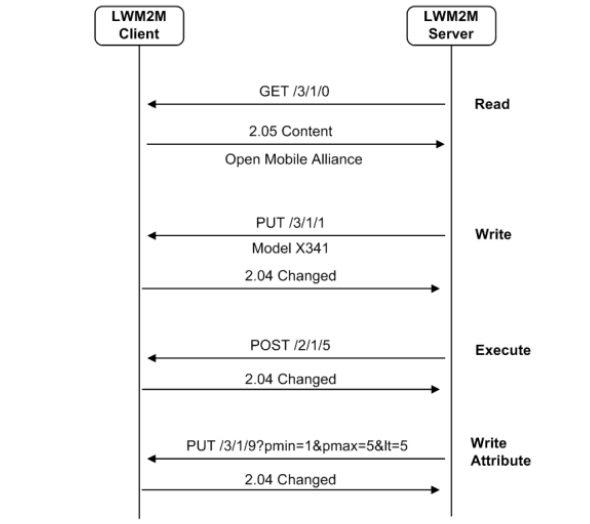
\includegraphics[scale=0.65]{../02_Analyse/images/lwm2m/command_diagram.png}
\caption{LwM2M Stack\cite{LwM2MInterfaces}}
\end{figure}
In der Grafik sieht man drei Beispielanfragen eines LwM2M-Servers.

Die erste Anfrage ist ein Read-Request. Der Server sendet ein GET auf die gewünschte Ressource, in diesem Beispiel ist dies 3/1/0 und wartet auf den Response. Der Client überprüft nun seine ACLs und wenn der Server berechtigt ist, sendet der Client ein Response  mit den Content zurück. Wenn die Ressource nicht vorhanden oder der Server nicht berechtigt ist, erhält der Server einen anderen Response als Content. Dies könnte zum Beispiel ''Not Found'' sein, falls die Ressource nicht vorhanden ist.

Der Write-Request ist sehr ähnlich aufgebaut. Anstelle eines GET-Requests sendet der Server ein PUT-Request. In diesem Request wird wieder die gewünschte Ressource-URL angesprochen und die zu schreibenden Daten werden direkt mit dem Request mitgesendet. Hier gibt der Client wieder mit ''Changed'' Antwort, falls alles in Ordnung ist.

Auch der Execute funktioniert gleich wie die anderen zwei Requests. Anstelle von GET oder PUT wird hier ein POST verwendet. Die Antwort beinhaltet wie beim Write-Requests ein ''Changed'' Status, damit der Server weiss, dass alles funktioniert hat.

\newpage

\subsubsection{Reporting - Allgemein}
LwM2M bietet neben den von Hand ausgeführten Read auch ein Observer an. Dieser wird mit dem Reporting Interface beschrieben. Reporting bietet dabei drei Funktionen. Observe, Notify und Cancel Observation. Mit dem Observe Befehl meldet sich ein Server beim Client und meldet sich an. Bei jeder Zustandsänderung der Ressource meldet sich der Client beim Server und sendet die neuen Daten an diesen Der Server kann so stetig wechselnde Daten sehr einfach überwachen, ohne die Ressource jedes mal von Hand upzudaten.
\subsubsection{Reporting - Ablauf}
Im Grunde wird hier ein normales Observer-Pattern umgesetzt. Der Server ist der Observer und der Client ist das Subject. Initiiert wird dieser Vorgang immer vom Server aus. 
\begin{figure}[H]
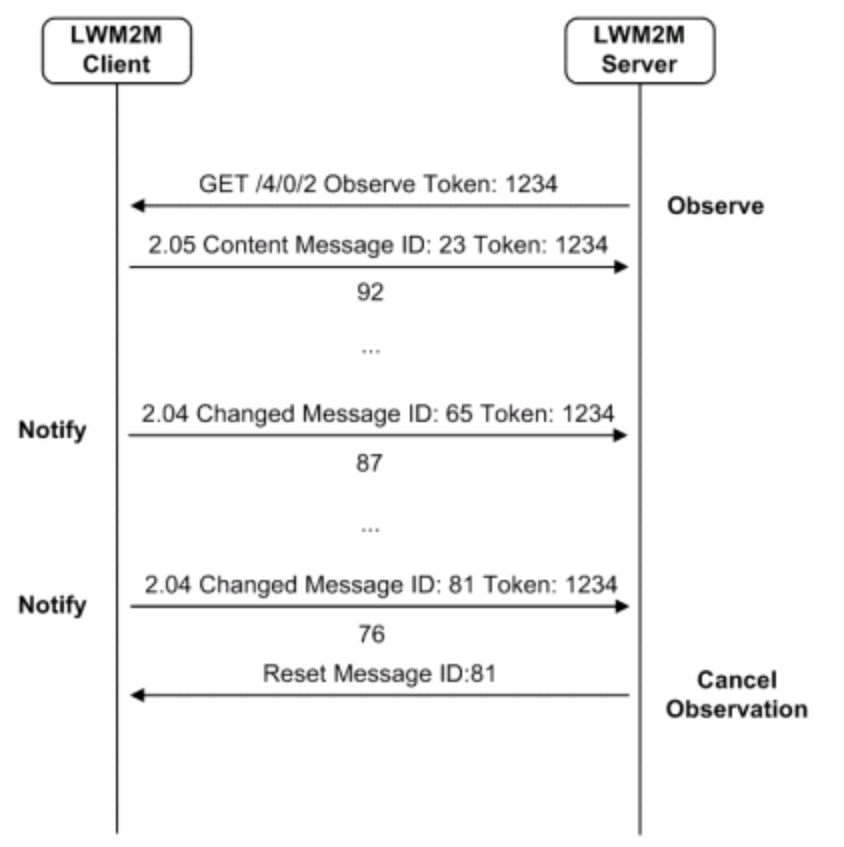
\includegraphics[scale=0.4]{../02_Analyse/images/lwm2m/report_diagram.png}
\caption{LwM2M Stack\cite{LwM2MInterfaces}}
\end{figure}
Um eine Ressource zu Überwachen, sendet der Server ein GET-Request an die gewünschte Ressource-URL mit einem Observe Token. Direkt nach dem Anmelden des Observers meldet der Client den aktuellen Wert der Ressource mit einer Content Message ID und dem Observer Token.

Bei jeder Änderung der Ressource erstellt der Client wieder ein neuer Response mit einer Changed Message ID und dem Token und sendet diese an alle Observer zurück.

Möchte der Server die Ressource nicht länger Überwachen, sendet der Server ein Reset zurück. Dieser Reset beinhaltet die letzte Changed Message ID. Hier im Beispiel sieht man dies ganz am Schluss der Grafik. So meldet sich der Server ab und erhält keine weiteren Notifikationen.

\subsection{Fazit}
\chapter{IoT-Security}
In diesem Kapitel sollen wichtige Aspekte der Security im IoT-Umfeld erarbeitet werden. Verschiedene Bereiche in der Architektur und deren Herausforderungen bezüglich Security erfordern unterschiedliche Massnahmen. Es wird versucht, zentrale Aspekte hervorzuheben, eine umfassende Behandlung ist in diesem Rahmen jedoch nicht möglich.
\section{Einführung}
Sicherheit ist im IoT-Bereich in den letzten Jahren immer wichtiger geworden. Viele Hersteller wollen ihre Produkte schnellstmöglich auf den Markt bringen und beachten Sicherheitsanforderungen zu wenig. Laut einer Studie von HP kamen bei den meisten Produkten schwerwiegende Sicherheitsbedenken auf.\cite{SecOverview} 

Die Vielfalt an Geräten bringt eine grosse Angriffsfläche mit sich. Verantwortliche müssen bei jedem Hersteller umfassende Sicherheitsanalysen durchführen. Im Gegensatz zu traditionellen Firmennetzwerken sind Netzwerke mit IoT-Devices schwieriger abzusichern. Bisher haben fast ausschliesslich Menschen die Kommunikation in Netzwerken verursacht. Maschine-zu-Maschine (M2M) Kommunikation ist in IoT-Netzwerken zentral. Menschen kommunizieren nur in seltenen Fällen (Konfiguration, Fehlerbehandlung, etc.) direkt mit den End-Devices. Die IoT-Devices haben dennoch ständige Kommunikation über das Netzwerk oder gar das Internet. Eine Kompromittierung dieser Systeme ist also theoretisch möglich.

\subsection{Folgen}
Die Vergangenheit hat gezeigt, dass Sicherheitsvorfälle schwerwiegende Folgen haben können. Reputationsverluste, Datenverluste, Industriespionage oder Systemausfälle durch Denial-of-Service (DoS) können Unternehmen beträchtlichen finanziellen Schaden zufügen. Wie seit einigen Jahren bekannt ist, haben selbst Regierungen von Weltmächten wie China, Russland oder die USA Interesse an der illegalen Beschaffung von Daten und Informationen. Die Motivation und technischen Fähigkeiten von Angreifern auf IT-Systeme sind sehr unterschiedlich. Ebenso unterscheiden sich die Sicherheitsbedürfnisse von Unternehmen stark.

Durch Entwicklungen im IoT-Umfeld muss damit gerechnet werden, dass IT-Systeme noch viel weiter als heute in Unternehmensprozessen eingebunden werden. Mit der Vision der Industrie 4.0 werden ganze Geschäftsprozesse vollautomatisiert und manuelle Tätigkeiten werden weitestgehend eliminiert. Wenn man von automatisierten Produktionsstätten ausgeht, kommen einige Gefahren zum Vorschein. Die Konkurrenz könnte beispielsweise durch gezielte Attacken auf ein Fertigungssystem Fehler einprogrammieren, welche zu grossen Rückrufaktionen und Reputationsverlusten führen könnten. Nochmals eine Stufe gefährlicher sind Attacken, welche Leib und Leben gefährden können. Denkt man an den medizinischen Bereich, könnten Patientensysteme, welche für die Medikation von Patienten zuständig sind, übernommen werden.

Es ist also ersichtlich, dass zu den herkömmlichen finanziellen Schäden bei IoT-Systemen Gefährdungen für Leib und Leben existieren können. Gesetzgeber wie auch Ingenieure müssen sich mit diesen wichtigen Herausforderungen intensiv befassen.

\subsection{Grobübersicht}  
Um eine möglichst übersichtliche Vorstellung von IoT-Security zu erhalten, werden vier grobe Architekturbereiche einzeln behandelt. Jeder dieser Bereiche birgt eigene Gefahren und benötigt unterschiedliche Massnahmen um die Informationssicherheit zu gewährleisten.
\begin{figure}[H]
\centering
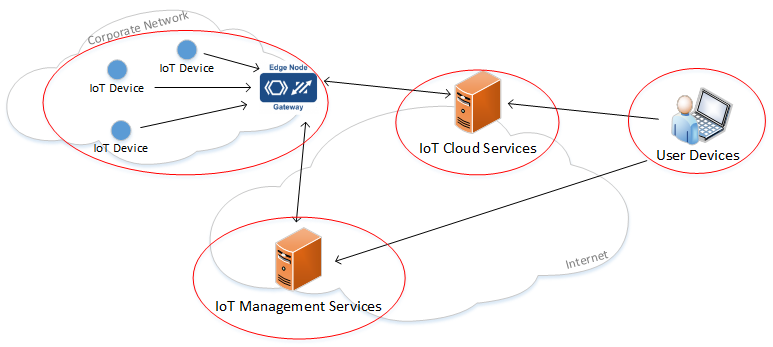
\includegraphics[scale=0.8]{../02_Analyse/images/security_overview.png}
\caption{Sicherheitszonen}
\end{figure}
\subsubsection{Device-Networks}
Device-Netzwerke beinhalten die IoT-Devices. Diese können sehr unterschiedlich aussehen. Denkbar wären Wireless Sensor Netzwerke (WSN), es könnten aber auch ''herkömmliche'', verkabelte Netzwerke sein. Die Heterogenität ist sehr gross, da nicht nur viele unterschiedliche Hersteller existieren, sondern auch die Arten der Kommunikation und die verwendeten Protokolle sich unterscheiden. 

\subsubsection{IoT-Cloud-Services}
IoT-Devices selbst kommunizieren häufig über Cloud-Services im Internet. Entweder stellen die Hersteller der Devices selbst Cloud-Services zur Verfügung, oder die Unternehmen entwickeln eigene Applikationen. Auf der einen Seite kommunizieren die Server mit den IoT-Devices oder deren Gateways, auf der anderen Seite werden die Services von End-Usern selbst benutzt. Sensordaten könnten auch über bereitgestellte APIs von anderen Cloud-Services konsumiert werden.

\subsubsection{User-Devices}
Benutzer selbst kommunizieren in den seltensten Fällen direkt mit IoT-Devices sondern über bereitgestellte Cloud Dienste. Häufige Devices sind PCs, Laptops und Mobilgeräte wie Smartphones oder Tablets.

\subsubsection{IoT-Management-Services}
Unternehmen möchten ihre IoT-Devices über einen zentralen Service verwalten. Häufig liefern Hersteller eigene Management Software, diese beschränken sich aber oft auf die Verwaltung von Geräten derselben Hersteller.
\newpage
\section{Informationssicherheit}
Nach dem Parker'schen Hexad befasst sich die Informationssicherheit grundlegend mit sechs Bereichen: \cite{ParkerianHexad}
\subsubsection{Vertraulichkeit (Confidentiality)}
Die Information muss geheim bleiben und darf von Unbefugten nicht einsehbar sein. Die Vertraulichkeit werden zum einen mittels kryptografischen Funktionen sichergestellt, zum anderen durch Berechtigungen. Informationen werden verschlüsselt, die vorgesehenen Entitäten sind im Besitz der Schlüssel um an die Informationen zu gelangen. Verschlüsseln von Informationen wird seit Tausenden von Jahren verwendet. Es existieren unterschiedliche Algorithmen und Schlüssellängen. Verwendete Techniken sollten regelmässig auf deren Aktualität und Sicherheit überprüft werden.
\subsubsection{Besitz oder Kontrolle (Possession or Control)}
Wenn ein Unbefugter in den Besitz oder die Kontrolle der Information bekommt so muss nicht zwangsweise die Vertraulichkeit verletzt sein. Wird beispielsweise ein Laptop oder eine Kreditkarte gestohlen, so erhält der Dieb diesen Zugriff, obwohl er nie vorgesehen wurde. Um sich vor diesen Gefahren zu schützen, empfiehlt sich eine Multi-Faktor Authentisierung, bei der Besitz und geheimes Wissen benötigt wird. 
\subsubsection{Integrität (Integrity)}
Bei der Einhaltung der Integrität möchte man die unbefugte oder unbemerkte Veränderung der Daten verhindern. Integritätschecks werden meistens mit kryptografischen Hashfunktionen durchgeführt. Dabei wird mittels einer mathematischen Einwegfunktion ein sogenannter Hashwert einer Eingangsinformation erstellt. Dieser Hashwert ist praktisch einmalig und schwierig reproduzierbar, weshalb bei einer Veränderung der Eingangsinformation ein anderer Hashwert resultiert. 
\subsubsection{Echtheit (Authenticity)}
Die Echtheit einer Information ist in vielen alltäglichen Bereichen wichtig. So möchte man sicherstellen, dass eine erhaltene Rechnung auch wirklich von der Firma stammt, von welcher man die Leistung bezogen hat. Bei E-Mails und dem zugrunde liegenden SMTP-Protokoll sind Probleme der Authentizität vielen Personen bekannt. Die Kryptografie hat Verfahren für digitale Signaturen hervorgebracht. Mit einem geheimen Schlüssel kann eine Information signiert werden, der dazugehörige öffentliche Schlüssel dient zur Verifikation der signierten Nachricht.
\subsubsection{Verfügbarkeit (Availability)}
Die Sicherheit ist ebenfalls nicht gewährleistet, wenn Informationen nicht verfügbar sind. Durch Denial-of-Service (DoS) Attacken, aber auch durch schlechte Planung oder unvorhergesehenen Ausfällen können Verfügbarkeitsprobleme auftreten. Durch Hochverfügbarkeitscluster können Ausfälle einzelner Knoten aufgefangen werden und die Wahrscheinlichkeit von Ausfällen drastisch reduziert werden.
\subsubsection{Nützlichkeit (Utility)}
Als Beispiel für die Verletzung dieses Aspekts kann man sich am besten ein vergessenes Passwort vorstellen. Sämtliche anderen Sicherheitsaspekte sind erfüllt, die Information ist trotzdem nicht zugänglich, da der benötigte Schlüssel (das Passwort) fehlt. Solche Fälle können durch Key-Recovery Mechanismen abgefangen werden. \cite{ParkerianHexadWiki}
\section{Device-Networks}
In diesem Unterkapitel werden Gefahren und Herausforderungen in Netzwerken mit IoT-Devices beschrieben.
\subsection{Device-Security}
\subsubsection{Software Versionen}
Ein wichtiger Aspekt für Unternehmen ist die Aktualität der verwendeten Software Versionen auf ihren IoT-Devices. Wie heute üblich, wird Software oft unfertig, mit Bugs und fehlenden Features ausgeliefert. Nach der Installation muss also schon fest mit kommenden Updates gerechnet werden. Die Unternehmen müssen also über ihre Softwarestände in den IoT-Systemen im Bilde sein und über die Möglichkeit von zeitnahen Updates verfügen. 

\subsubsection{Physischer Zugriff}
Wie bei vielen anderen Geräten sollte auch bei IoT-Devices der physische Zugang nur autorisierten Personen vorbehalten sein. Sonst könnte beispielsweise ein Sensor manipuliert werden, der falsche Daten liefert.

\subsubsection{Authentifizierung und Autorisierung}
Da ein IoT-Device über das Internet kommuniziert, sollten Zugriffe authentifiziert und autorisiert werden. Durch unbefugten Zugriff können entweder potenziell sensible Sensordaten gelesen werden. Ausserdem besteht die Möglichkeit, einem Botnetz beizutreten, was mit geschützten Zugriffen teilweise entschärft werden kann. Es sollten ausserdem Mechanismen vorgesehen werden, welche zuständige Personen bei zu häufigen Fehlversuchen benachrichtigen, da potenziell eine Attacke vorliegen könnte.
 \newpage
\subsection{Netzwerksicherheit}
\subsubsection{Bootstrapping}
In der Bootstrapping-Phase betritt ein neues IoT-Device ein bestehendes Netzwerk. Eine Security-Association (SA) zwischen dem IoT-Device und dem Netzwerk, resp. deren Devices muss erstellt werden. Als Betreiber des Netzwerks muss man sicherstellen, dass nur vorgesehene Devices beitreten können, deshalb ist eine Authentisierung sehr wichtig. Das IoT-Device muss im Gegensatz dem Netzwerk vertrauen. Ein Server kann über Protokolle wie beispielsweise EAP neue Devices authentisieren.
\begin{figure}[H]
\centering
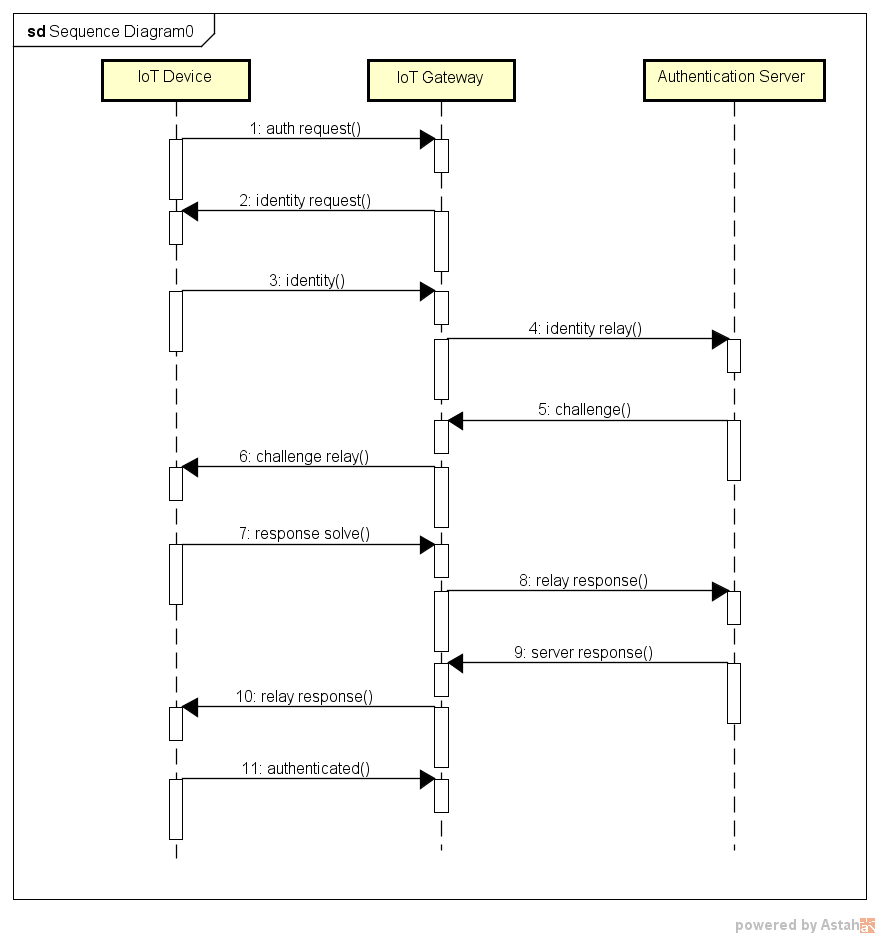
\includegraphics[scale=0.6]{../02_Analyse/images/deviceauthentication.png}
\caption{Schema möglicher Deviceauthentisierung}
\end{figure}
Im Gegensatz zu herkömmlichen Geräten, bei denen die Identität beispielsweise durch die Eingabe eines Passworts oder der Verteilung von Zertifikaten mittels einer PKI festgestellt werden kann, kommen bei IoT-Geräten erschwerende Hürden hinzu. \cite{IoTSecurityChallenges} So könnten Devices beispielsweise über keine direkten Eingabemöglichkeiten-, oder zu wenig Rechenleistung für herkömmliche asymmetrische Kryptografie verfügen.

\subsubsection{Verschlüsselung}
Weder das HTTP-, noch das CoAP-Protokoll haben eine eigene Verschlüsselung des Payloads vorgesehen. Seit langer Zeit wird für HTTP SSL, respektive TLS verwendet, um die Kommunikation zwischen zwei Devices zu verschlüsseln. TLS verschlüsselt die gesamten Pakete in der Applikationsschicht, Protokolle unterhalb der Applikationsschicht sind weiterhin im Klartext verfügbar. 

IoT-Devices arbeiten häufig mit CoAP anstatt HTTP. Wie in Kapitel \ref{sec:iotkomm} beschrieben, arbeitet CoAP im Gegensatz zu HTTP mit UDP anstelle von TCP. TLS selbst benötigt jedoch TCP als Transportprotokoll, weshalb sich dieses Verfahren also nicht für CoAP eignet.

Aus diesen Gründen musste ein neues Verschlüsselungsprotokoll DTLS (Datagram Transport Layer Security) entwickelt werden, welches ''TLS'' über UDP ermöglicht. Die Unterschiede von TLS zu DTLS sind gering. Einfach betrachtet erledigen die Protokolle die gleichen Aufgaben.

\begin{figure}[H]
\centering
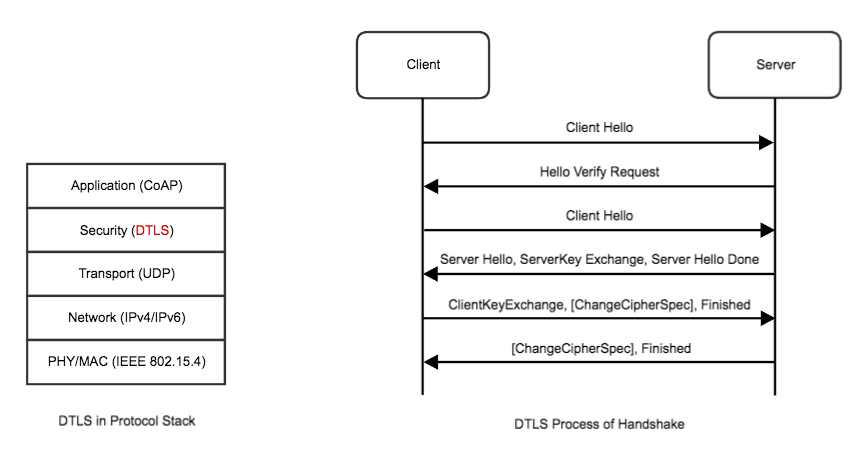
\includegraphics[scale=0.5]{../02_Analyse/images/coap_dtls_diagram.png}
\caption{DTLS Sequenz Diagramm} \cite{DTLSDiagram}
\end{figure}
\newpage
\section{Cloud-Services}
In diesem Unterkapitel werden sicherheitsrelevante Aspekte für IoT-Cloud-Dienste behandelt. Neben den behandelten Themen müssen viele weitere Aspekte, welche für übrige Internetdienste gelten auch eingehalten werden.
\subsection{Bedeutung}
IoT-Cloud-Dienste kommunizieren mit Sensoren und empfangen deren Daten. IoT-Cloud-Applikationen steuern ganze Geschäftsprozesse, deshalb sind sie in diesem Umfeld oft businesskritisch. Cloud-Services kommunizieren auf der einen Seite mit IoT-Devices (M2M-Kommunikation), auf der anderen Seite mit End-User Devices.  
\begin{figure}[H]
\centering
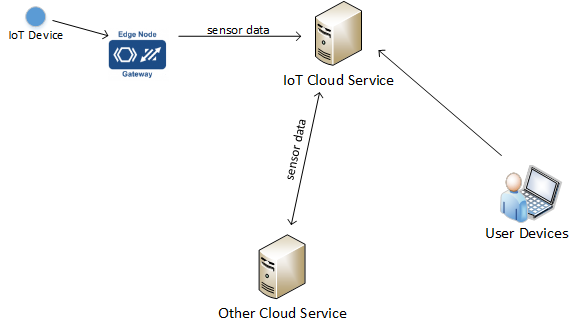
\includegraphics[scale=0.8]{../02_Analyse/images/cloudservices.png}
\caption{IoT-Cloud-Service Übersicht}
\end{figure}

Wie in der Einführung bereits erwähnt, können die Folgen von Ausfällen je nach Applikation sehr unterschiedlich sein. Eintrittswahrscheinlichkeiten und Schadensausmasse müssen in einer Risikoanalyse bewertet werden, damit geeignete Massnahmen getroffen werden können. So benötigen Patientensysteme in Spitälern weitaus mehr Sicherheitsmassnahmen als Pflanzenüberwachungssysteme in Gewächshäusern.

\subsection{API-Security}
Kommunikation und Austausch von Daten erfolgen über bereitgestellte APIs. Sämtliche API Zugriffe müssen zuerst authentifiziert werden, ansonsten können möglicherweise geheime Daten abgefragt-, oder gar fehlerhafte und schädliche Inputs eingegeben werden. Mittels Berechtigungen sollte festgelegt werden, wer auf welche Daten zugreifen darf. 
\newpage
\subsection{Korrektheit}
Je nach Sensitivität der Cloud-Applikation müssen Softwareentwickler ein erhöhtes Augenmerk auf die Korrektheit der Software legen. Die Vergangenheit hat gezeigt, dass Softwarefehler wie falsches Exception Handling oder Race Conditions weitreichende Folgen haben können. Hängt beispielsweise eine ganze Produktionskette von der Cloud-Applikation ab, so könnte ein Absturz innert kürzester Zeit einen sehr hohen finanziellen Schaden bedeuten. 

\subsection{Verfügbarkeit}
Wie bei herkömmlichen Servern muss auch bei Applikationsserver im IoT-Bereich auf die Verfügbarkeit geachtet werden. Es gibt potenziell viele Vorfälle, welche die Verfügbarkeit beeinträchtigen könnten. Als wirksamste Methode empfiehlt sich eine redundante Auslegung der wichtigsten Komponenten.

\section{User-Devices}
In diesem Unterkapitel werden Gefahren und Massnahmen für End-User Devices behandelt. Über Geräte PCs, Notebooks, Tablets oder Smartphones werden IoT-Services konsumiert. Für Unternehmen stellen sich seit dem ''bring-your-own-device''-Zeitalter die Herausforderung, dass nicht nur User Devices im Firmenbesitz auf interne Anwendungen zugreifen. Network-Access-Control-Systeme überprüfen diverse Attribute wie beispielsweise Virendefinitionen von Devices an einem Enforcement-Point, bevor in den geschützten Bereich zugegriffen werden kann. Grundsätzlich unterscheiden sich die empfohlenen Security-Massnahmen für User-Devices für IoT-Anwendungen nicht von herkömmlichen Systemen, da potenzielle Schadensausmasse jedoch höher sind, sollten empfohlene Massnahmen konsequent umgesetzt werden.

\subsection{Client-Applikationen}
Unterschiedliche Arten von Client-Applikationen sind für IoT-Anwendungen denkbar. Herkömmlich installierte Desktop-Programme für Windows-Betriebssysteme verlieren an Bedeutung. Web- und Mobil-Applikationen haben in den letzten Jahren stark zugenommen. 

Ein Benutzer muss sich an der Client-Anwendung authentisieren. Wie hinlänglich bekannt, muss die Authentifizierung an einem vorgesehenen Server stattfinden. Für sensitive Anwendungen sollten Multi-Faktor-Authentifizierungslösungen eingesetzt werden. Neuere Mobilgeräte und Notebooks verfügen häufig über Fingerabdruckscanner, es wären aber auch SMS-Tokens oder Smartcards als weitere Möglichkeit neben Passwörtern denkbar.

Mobile Geräte werden oft verloren oder gestohlen. Sobald eine Session beendet wurde, sollte eine erneute Authentifizierung verlangt werden. Es sollte ein möglichst kurzes Session-Timeout gewählt werden, damit beim Vergessen des Logouts fremde Personen keinen Zugriff erhalten können.

Viele sicherheitsrelevante Überprüfungen von Anwendungen wie Input-Validierung müssen serverseitig implementiert werden, da man clientseitige Security-Checks leicht umgehen kann. Es gibt jedoch Angriffe wie Phishing oder Social Engineering, welche selbst serverseitig nicht abgefangen werden können. Gegen solche Angriffe schützt man sich am besten mit Benutzerschulungen.

\section{Management-Server}
In diesem Abschnitt wird Security für Management Server behandelt. Ziel dieses Projektes ist ein Prototyp eines Management Servers zu erstellen. Es ist wichtig, bereits vorgängig Security fest einzuplanen, da die Kosten für Security-Vorfälle mit der Zeit zunehmen.

\subsection{Bedeutung}
Management Server sind für Unternehmen sicherheitskritische Systeme. Sie gelten als besonders schützenswert, da viele Applikationen und ganze Geschäftsprozesse abhängig sein könnten. Ist der IoT-Management-Server kompromittiert, so erhält der Angreifer eine Komplettübersicht des gesamten IoT-Systems eines Unternehmens. Als Angreifer könnte man dann beispielsweise versucht sein, Devices herunterzufahren, fehlerhafte Konfigurationen einzuspielen, oder sensitive Informationen zu gewinnen.

\subsection{User Interface}
Es muss die Frage gestellt werden, ob Zugriffe aus dem Internet notwendig sind. Allenfalls könnten externe Benutzer über ein Virtual Private Network (VPN) zugreifen. Angreifer aus dem Internet hätten somit keinen direkten Zugriff ausserhalb des Firmennetzwerks.

Da sensitive Informationen wie Kennwörter und weitere Daten übertragen werden, sollte der Netzwerkverkehr (auch firmenintern) verschlüsselt werden. Wird zum Beispiel ein Web-Interface verwendet, so sollte jeglicher Verkehr über das TLS gesicherte HTTPS-Protokoll geschehen. Unverschlüsselte Verbindungen dürfen nicht erlaubt werden.

Inputvalidierung ist bei Applikationen enorm wichtig. Sicherheitsrelevante Validierungen müssen zwingend serverseitig implementiert werden. Durch saubere Input Validierungen werden häufige Angriffe wie Code Injection, XSS und CSRF Attacken verhindert.

\subsection{Devicekommunikation}
Der Management Server kommuniziert über eigene Sessions mit IoT-Devices. Meldet sich ein Device beim Management Server, so muss dieser zuerst überprüfen, ob das Device berechtigt ist, um mit dem Management Server zu kommunizieren. Auf dem Server könnte beispielsweise ein Passwort hinterlegt werden, welches neuen Devices bekannt sein muss. 

Man könnte auf dem Server auch vertrauenswürdige Root Zertifikate hinterlegen. So könnten Clients, welche Zertifikate von einem dieser vertrauten Root Zertifikate ausgestellt erhalten haben auf den Management Server zugreifen. Der lokale Bootstrap-Server könnte solche Clientzertifikate an die IoT-Devices ausstellen.

\begin{figure}[H]
\centering
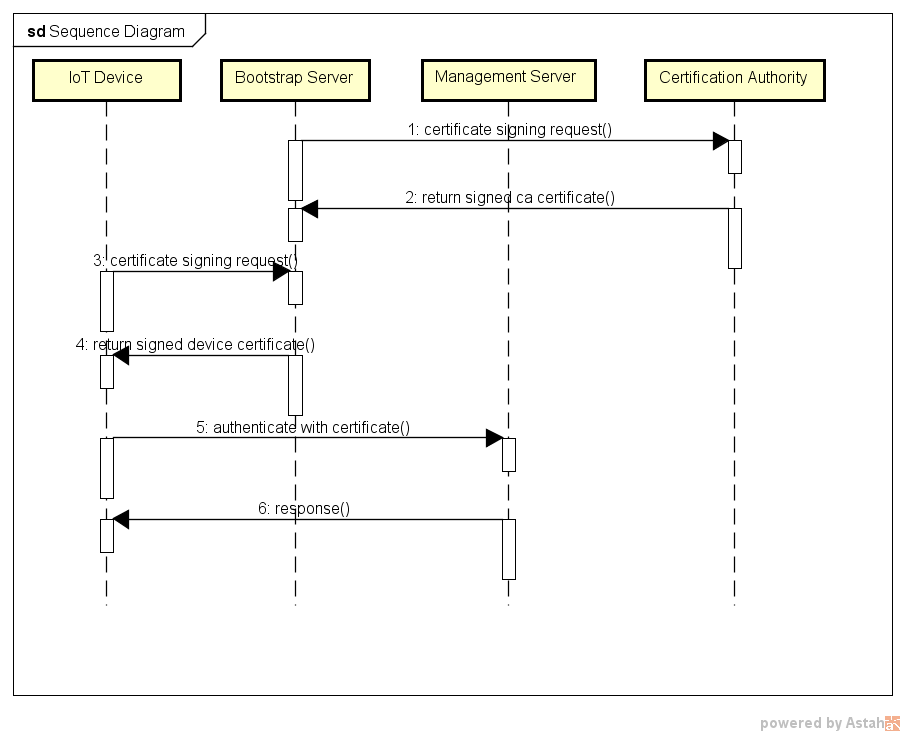
\includegraphics[scale=0.7]{../02_Analyse/images/certificateauthentication.png}
\caption{Authentisierung mit Zertifikaten}
\end{figure}

IoT-Devices übermitteln unter Umständen sensitive Daten an den Management Server. Die Kommunikation muss deshalb verschlüsselt werden.

\subsection{Server}
Die Management Applikation sollte über ein sicheres Authentifizierungsverfahren verfügen. Für kritische Applikationen lohnt sich eine Zwei-Faktor-Authentifizierung. Viele Benutzer verwenden überall die selben Kennwörter oder schreiben sie sich auf, weshalb ein Verlust des Kennworts nicht sehr unwahrscheinlich ist. Durch eine zweite Authentifizierungshürde verbessert sich die Sicherheit markant.

Bereitgestellte APIs müssen geschützt sein. Nur authentifizierte Benutzer sollten zugreifen dürfen. Die Kommunikation über diese APIs muss gesichert sein, dass keine schädlichen Daten übertragen werden können. 

Auch für Management Server ist die Verfügbarkeit wichtig. Hardwarekomponenten sollten redundant vorhanden sein. Der Applikationsserver sollte regelmässig gesichert sein, sodass im Totalausfall durch einen Restore die Downtime möglichst kurz gehalten wird.





\chapter{Requirements}
\section{Allgemeine Beschreibung}
\subsection{Produktperspektive}
Mit Internet of Things sind eine Vielzahl neuartige Devices entstanden. Während in herkömmlichen Netzwerken hauptsächlich Personal Computer, Notebooks, Server usw. verwaltet werden mussten, so bringen IoT Devices den IT-Abteilungen neue Herausforderungen. Zum einen dürfte die Anzahl Geräte gegenüber herkömmlichen Computer deutlich ansteigen, zum anderen sind IoT Devices in Sachen Funktionalität und Rechenleistung, sowie auch der Netzwerkbandbreite deutlich beschränkt. 

Mit <insert Application Name here> soll eine Management Applikation bereitgestellt werden, um eine Vielzahl unterschiedlicher IoT Devices administrieren zu können. 
\subsection{Produkfunktionen}
<insert Application Name here> soll den Benutzern erlauben, IoT Geräte zu verwalten. Die Aufgaben reichen vom Erfassen und Discovery von Devices über die Konfigurationsverwaltung und Softwareverteilung bis zu Backup und Restore. Ausserdem sollen Management-relevante Kommandos auf Devices ausgeführt- und Security Aspekte beachtet werden. Die Details zu den Produktfunktionen sind den Use Cases zu entnehmen.

\subsection{Benutzer Charakteristik}
Zielpersonen der Applikation sind Betreiber von IoT Devices. Dies können im Enterprise Umfeld IT-Mitarbeiter in operationeller Funktion-, oder auch Softwareentwickler für IoT Applikationen sein. Heimanwender können bei entsprechenden Kenntnissen ebenfalls zur Zielgruppe gehören. Es werden solide Grundkenntnisse in TCP/IP Netzwerken sowie Verständnis der verwendeten IoT Architekturen und Devices vorausgesetzt. 
\subsection{Einschränkungen}
Evtl. Browser Einschränkungen und bestimmte Use Cases, müsste nach Prototyp nochmals definiert werden
\section{Use Cases}
\subsection{Use Cases Diagramm}
%\includegraphics[scale=0.52]{figures/UseCase_Diagram}
\subsection{Aktoren}
Der Benutzer der Applikation ist in diesem System der einzige primäre Aktor.
\subsection{Beschreibungen (Casual)}
\subsubsection{Benutzer CRUD}
\mbox{}
\begin{longtable}{| p{4cm} | p{11.7cm} |}
 \hline
 \textbf{Name} & • \\ \hline 
 \textbf{Beschreibung} & • \\ \hline 
 \textbf{Preconditions} & • \\ \hline 
 \textbf{Postconditions} & • \\ \hline 
 \textbf{Main Success Scenario} & • \\ \hline 
 \textbf{Extensions} & • \\ \hline 
 \end{longtable}

\subsubsection{discover Device}
\mbox{}
\begin{longtable}{| p{4cm} | p{11.7cm} |}
 \hline
 \textbf{Name} & Device discover \\ \hline 
 \textbf{Beschreibung} & Der Benutzer möchte ein IoT Device finden. Entsprechende IoT Devices sollen dem Benutzer zur Adoption aufgelistet werden. \\ \hline 
 \textbf{Preconditions} & • \\ \hline 
 \textbf{Postconditions} & • \\ \hline 
 \textbf{Main Success Scenario} & • \\ \hline 
 \textbf{Extensions} & • \\ \hline 
\end{longtable}

\subsubsection{Device erfassen}
\mbox{}
\begin{longtable}{| p{4cm} | p{11.7cm} |}
 \hline
 \textbf{Name} & • \\ \hline 
 \textbf{Beschreibung} & Der Benutzer möchte ein IoT Device manuell hinzufügen. Der Endpunkt ist dem Benutzer bekannt. \\ \hline 
 \textbf{Preconditions} & • \\ \hline 
 \textbf{Postconditions} & • \\ \hline 
 \textbf{Main Success Scenario} & • \\ \hline 
 \textbf{Extensions} & • \\ \hline 
 \end{longtable}
 
\subsubsection{Device assoziieren}
\mbox{}
\begin{longtable}{| p{4cm} | p{11.7cm} |}
 \hline
 \textbf{Name} & Device assoziieren \\ \hline 
 \textbf{Beschreibung} & Der Benutzer möchte ein- oder mehrere IoT Device(s) verwalten. Dazu muss er das gefundene Device in das System adoptieren. \\ \hline 
 \textbf{Preconditions} & • \\ \hline 
 \textbf{Postconditions} & • \\ \hline 
 \textbf{Main Success Scenario} & • \\ \hline 
 \textbf{Extensions} & • \\ \hline 
 \end{longtable}
 
\subsubsection{Device CRUD}
\mbox{}
\begin{longtable}{| p{4cm} | p{11.7cm} |}
 \hline
 \textbf{Name} & • \\ \hline 
 \textbf{Beschreibung} & • \\ \hline 
 \textbf{Preconditions} & • \\ \hline 
 \textbf{Postconditions} & • \\ \hline 
 \textbf{Main Success Scenario} & • \\ \hline 
 \textbf{Extensions} & • \\ \hline 
 \end{longtable}
 
\subsubsection{Device abfragen}
\mbox{}
\begin{longtable}{| p{4cm} | p{11.7cm} |}
 \hline
 \textbf{Name} & • \\ \hline 
 \textbf{Beschreibung} & • \\ \hline 
 \textbf{Preconditions} & • \\ \hline 
 \textbf{Postconditions} & • \\ \hline 
 \textbf{Main Success Scenario} & • \\ \hline 
 \textbf{Extensions} & • \\ \hline 
 \end{longtable}
 
\subsubsection{Konfiguration speichern}
\mbox{}
\begin{longtable}{| p{4cm} | p{11.7cm} |}
 \hline
 \textbf{Name} & • \\ \hline 
 \textbf{Beschreibung} & • \\ \hline 
 \textbf{Preconditions} & • \\ \hline 
 \textbf{Postconditions} & • \\ \hline 
 \textbf{Main Success Scenario} & • \\ \hline 
 \textbf{Extensions} & • \\ \hline 
 \end{longtable}
 
\subsubsection{Konfiguration verteilen}
\mbox{}
\begin{longtable}{| p{4cm} | p{11.7cm} |}
 \hline
 \textbf{Name} & • \\ \hline 
 \textbf{Beschreibung} & • \\ \hline 
 \textbf{Preconditions} & • \\ \hline 
 \textbf{Postconditions} & • \\ \hline 
 \textbf{Main Success Scenario} & • \\ \hline 
 \textbf{Extensions} & • \\ \hline 
 \end{longtable}
 
\subsubsection{Konfiguration anzeigen}
\mbox{}
\begin{longtable}{| p{4cm} | p{11.7cm} |}
 \hline
 \textbf{Name} & • \\ \hline 
 \textbf{Beschreibung} & • \\ \hline 
 \textbf{Preconditions} & • \\ \hline 
 \textbf{Postconditions} & • \\ \hline 
 \textbf{Main Success Scenario} & • \\ \hline 
 \textbf{Extensions} & • \\ \hline 
 \end{longtable}
 
\subsubsection{Software speichern}
\mbox{}
\begin{longtable}{| p{4cm} | p{11.7cm} |}
 \hline
 \textbf{Name} & • \\ \hline 
 \textbf{Beschreibung} & • \\ \hline 
 \textbf{Preconditions} & • \\ \hline 
 \textbf{Postconditions} & • \\ \hline 
 \textbf{Main Success Scenario} & • \\ \hline 
 \textbf{Extensions} & • \\ \hline 
 \end{longtable}
 
\subsubsection{Software verteilen}
\mbox{}
\begin{longtable}{| p{4cm} | p{11.7cm} |}
 \hline
 \textbf{Name} & • \\ \hline 
 \textbf{Beschreibung} & • \\ \hline 
 \textbf{Preconditions} & • \\ \hline 
 \textbf{Postconditions} & • \\ \hline 
 \textbf{Main Success Scenario} & • \\ \hline 
 \textbf{Extensions} & • \\ \hline 
 \end{longtable}
 
\subsubsection{Device sichern}
\mbox{}
\begin{longtable}{| p{4cm} | p{11.7cm} |}
 \hline
 \textbf{Name} & • \\ \hline 
 \textbf{Beschreibung} & • \\ \hline 
 \textbf{Preconditions} & • \\ \hline 
 \textbf{Postconditions} & • \\ \hline 
 \textbf{Main Success Scenario} & • \\ \hline 
 \textbf{Extensions} & • \\ \hline 
 \end{longtable}
 
\subsubsection{Device restoren}
\mbox{}
\begin{longtable}{| p{4cm} | p{11.7cm} |}
 \hline
 \textbf{Name} & • \\ \hline 
 \textbf{Beschreibung} & • \\ \hline 
 \textbf{Preconditions} & • \\ \hline 
 \textbf{Postconditions} & • \\ \hline 
 \textbf{Main Success Scenario} & • \\ \hline 
 \textbf{Extensions} & • \\ \hline 
 \end{longtable}
 
\subsubsection{Device authentisieren}
\mbox{}
\begin{longtable}{| p{4cm} | p{11.7cm} |}
 \hline
 \textbf{Name} & • \\ \hline 
 \textbf{Beschreibung} & • \\ \hline 
 \textbf{Preconditions} & • \\ \hline 
 \textbf{Postconditions} & • \\ \hline 
 \textbf{Main Success Scenario} & • \\ \hline 
 \textbf{Extensions} & • \\ \hline 
 \end{longtable}
 
\subsubsection{Schlüssel verwalten}
\mbox{}
\begin{longtable}{| p{4cm} | p{11.7cm} |}
 \hline
 \textbf{Name} & • \\ \hline 
 \textbf{Beschreibung} & • \\ \hline 
 \textbf{Preconditions} & • \\ \hline 
 \textbf{Postconditions} & • \\ \hline 
 \textbf{Main Success Scenario} & • \\ \hline 
 \textbf{Extensions} & • \\ \hline 
 \end{longtable}
 
\subsubsection{Zertifikate speichern}
\mbox{}
\begin{longtable}{| p{4cm} | p{11.7cm} |}
 \hline
 \textbf{Name} & • \\ \hline 
 \textbf{Beschreibung} & • \\ \hline 
 \textbf{Preconditions} & • \\ \hline 
 \textbf{Postconditions} & • \\ \hline 
 \textbf{Main Success Scenario} & • \\ \hline 
 \textbf{Extensions} & • \\ \hline 
 \end{longtable}
 
\subsubsection{Zertifikate verteilen}
\mbox{}
\begin{longtable}{| p{4cm} | p{11.7cm} |}
 \hline
 \textbf{Name} & • \\ \hline 
 \textbf{Beschreibung} & • \\ \hline 
 \textbf{Preconditions} & • \\ \hline 
 \textbf{Postconditions} & • \\ \hline 
 \textbf{Main Success Scenario} & • \\ \hline 
 \textbf{Extensions} & • \\ \hline 
 \end{longtable}
 
\subsubsection{Device Kommandos ausführen}
\mbox{}
\begin{longtable}{| p{4cm} | p{11.7cm} |}
 \hline
 \textbf{Name} & • \\ \hline 
 \textbf{Beschreibung} & • \\ \hline 
 \textbf{Preconditions} & • \\ \hline 
 \textbf{Postconditions} & • \\ \hline 
 \textbf{Main Success Scenario} & • \\ \hline 
 \textbf{Extensions} & • \\ \hline 
\end{longtable}


 
 

\section{Nichtfunktionale Anforderungen}
In diesem Kapitel behandeln wir die nichtfunktionalen Anforderungen an das Projekt. Wir behandeln Aspekte und Anforderungen aus den Bereichen Qualität, Schnittstellen und Randbedingungen.
\subsection{Qualität}
Bei der Softwarequalität stützen wir uns auf die ISO/IEC 9126 Norm. Es werden die Merkmale Funktionalität, Zuverlässigkeit, Benutzbarkeit, Effizienz, Wartbarkeit und Übertragbarkeit aufgeführt.
\subsubsection{Funktionalität}
Netzwerkdevices können von vielen unterschiedlichen Herstellern kommen. Diese Hersteller verwenden unterschiedliche Syntax und Ausgabeformate. Um die Funktionalität best möglich sicherzustellen, wird die Herstellerunterstützung vorerst stark eingeschränkt. Vorgesehen sind vorerst Cisco Netzwerkdevices und Linux Hosts.
\subsubsection{Zuverlässigkeit}
Tests sind wichtig und nützlich, jedoch nicht Business kritisch bei einem möglichen Ausfall. Es muss vor allem darauf geachtet werden, dass bei ssh Verbindungen ein sauberes Exception Handling implementiert wird, falls beim Verbindungsaufbau oder bei abgesetzten Kommandos etwas schief geht. Es müssen für gewisse Tests auch Timeouts eingeplant werden, damit das Programm nicht unendlich lange blockieren kann.
\subsubsection{Benutzbarkeit}
Wir möchten ein schmales User Interface auf Konsolen Ebene bieten. Der Anwender muss über Kenntnisse auf der Linux bash verfügen. Mittels eingebauter Hilfe soll es versierten Benutzern möglich sein, die Software zu verwenden.
\subsubsection{Effizienz}
Die Effizienz ist sehr stark von den getesteten Devices und den abgesetzten Kommandos abhängig. 
\subsubsection{Wartbarkeit}
Eigene Test Cases sollen mit den notwendigen Kenntnissen selbst ergänzt werden können. Command-Mapping und Outputs müssen bekannt sein, dann ist eine Erweiterung des Funktionsumfangs der Test Cases denkbar.
\subsubsection{Übertragbarkeit}
Die Übertragbarkeit auf andere Plattformen oder Hersteller ist schwierig und vorerst nicht vorgesehen.

\subsection{Schnittstellen}
\subsubsection{Benutzerschnittstellen}
Die Steuerung des Programms ist mittels Tastatur über die Linux bash vorgesehen.

\subsubsection{Netzwerkschnittstellen}
Im Programm können alle Devices verwendet werden, welche über ein lokales Netzwerkinterface erreichbar sind.

\subsection{Sicherheit}
Um auf Devices verbinden zu können, muss man sich auf diesen authentifizieren. Administrator Zugänge müssen deshalb best möglichst geschützt sein. Die Übertragung muss verschlüsselt sein (ssh) und die Passwörter dürfen, wenn überhaupt, nur mittels sicherem Hashverfahren abgelegt werden.
\chapter{Technologie Evaluation}
In diesem Kapitel werden relevante Technologien und Frameworks, welche das Front-End, Back-End, sowie die Datenbank betreffen, evaluiert. Für jeden dieser Bereiche wurden Kriterien erarbeitet. Die Auswahl geschieht aufgrund der Bewertung anhand dieser Kriterien.

\section{Back-End}
Die Entscheidung des Frameworks für das Back-End ist von grosser Tragweite. Heutzutage existieren einige beliebte Frameworks um Web Applikationen zu erstellen. Die zu verwendende Programmiersprache ist bei vielen Frameworks ebenfalls unterschiedlich und sollte berücksichtigt werden.

\subsection{Kriterien}
\begin{itemize}
\item Open-Source
\item Gute Dokumentation und Unterstützung durch die Community
\item Einfache Bedienung und schnelle Einarbeitung
\item Performance / Skalierbarkeit
\item Libraries für IoT-Kommunikationsprotokolle
\item Kenntnisse der Programmiersprache
\end{itemize}

\begin{longtable}{| p{4cm} | p{11.7cm} |}
\hline
\textbf{Node.js}\newline

\includegraphics[width=0.25\columnwidth]{../03_Design/images/nodejs_logo.png} & Node.js ist eine Plattform für serverseitiges JavaScript. Das I/O-Handling ist event-driven und nicht-blockierend. Jeder Node.js Prozess ist single-threaded. Node.js hat viele Erweiterungsmodule wie z.B. Express um Web Applikationen zu erstellen. Für Web Applikationen ist Node.js mit Express besonders gut geeignet, da auf Client- und Serverseite mit JavaScript gearbeitet werden kann. Die Anzahl möglicher Verbindungen könnten trotz Single-Threading gut gehandled werden da die Anfragen asynchron mit einem Callback an die Devices gesendet werden, der aktive Thread würde somit nicht blockieren.
\newline
\newline
\textbf{Vorteile} \newline
\tabitem Einfacher Einstieg \newline
\tabitem Weite Verbreitung und gute Community-Unterstützung \newline
\tabitem Gute Skalierbarkeit (non-blocking) \newline
\tabitem Grundkenntnisse beim Entwicklerteam vorhanden \newline
\tabitem Gleiche Programmiersprache beim Front- und Backen \newline
\textbf{Nachteile} \newline
\tabitem Kein Multi-Threading \newline
\tabitem Interpretierte Skriptsprache \newline
\tabitem Schwache Objektorientierung (kein Polymorphismus, Duck-Typing, etc.)\\ \hline
\textbf{Spring MVC}\newline

\includegraphics[width=0.25\columnwidth]{../03_Design/images/spring_logo.png}
& Spring MVC wird verwendet um dynamische Webseiten mit Java Servlets zu erstellen. Dependency Injection und aspektorientierte Programmierung sind ebenfalls unterstützt. Konfigurationen über XML und Java Annotations unterstützen den Entwickler beim Erstellen von MVC Web-Applikationen. Die Library-Unterstützung für IoT-spezifische Kommunikationsprotokolle wie beispielsweise CoAP sind bei Java EE hervorragend. Java unterstützt sowohl Multi-Threading, als auch non-blocking I/O. Gleichzeitige Verbindungen zu Devices könnten in eigene Threads ausgelagert werden, um nicht das gesamte Back-End zu blockieren.
\newline
\newline
\textbf{Vorteile} \newline
\tabitem Weite Verbreitung und gute Community-Unterstützung \newline
\tabitem Gute Skalierbarkeit (Multi-Threading) \newline
\tabitem Gute Java Programmierkenntnisse beim Entwicklerteam vorhanden \newline
\tabitem Kompilierte Sprache \newline
\tabitem Starke Objektorientierung (Polymorphismus, Type-Safety, etc.) \newline
\tabitem Dependency-Injection Unterstützung \newline
\textbf{Nachteile} \newline
\tabitem Umgang mit Spring MVC müsste vom Entwicklerteam erlernt werden \newline
\tabitem Unterschiedliche Sprachen für Front- und Back-End
\\ \hline 
\end{longtable}

\subsection{Skalierbarkeit}
Da potenziell viele Devices über die Applikation verwaltet werden könnten ist die Skalierbarkeit von grosser Bedeutung. Die Art der Verbindungen unterscheiden sich. Während die Anzahl gleichzeitiger Verbindungen über das Front-End zum Server (concurrent users) sehr gering sein wird, besteht die Möglichkeit, dass hunderte oder gar tausende IoT-Devices verbunden sind.

Es besteht jedoch nicht die Notwendigkeit, dass während der Nutzungsdauer alle diese Verbindungen aufgebaut und offen gehalten werden. Es ist damit zu rechnen, dass niemals mehr als 100 gleichzeitige Verbindungen zu unterschiedlichen Devices existieren. 

\subsection{Entscheidung}
Die Entscheidung fiel auf Spring MVC. Eine Implementation mittels Node.js und Express wäre ebenfalls denkbar, da alle Anforderungen und Restriktionen erfüllt werden könnten. Auch andere Frameworks wie Django oder Ruby on Rails würden ebenfalls in Frage kommen, wurden aber nicht berücksichtigt da keine oder nur kaum Vorkenntnisse beim Entwicklerteam vorhanden waren.

Ausschlaggebend für die Auswahl von Spring MVC ist die zugrundeliegende Programmiersprache Java. Die Unterstützung von Klassen, Vererbung und Polymorphie sowie die grosse Unterstützung von Tools und Plugins ermöglichen eine angenehmere und übersichtlichere Entwicklung. Durch die Unterstützung mittels XML Konfigurationen und Java Annotations werden die Entwickler mit Spring MVC hervorragend unterstützt.

\newpage
\section{Front-End}
Das Front-End der Applikation muss dem Benutzer auf eine einfache und übersichtliche Weise die Interaktion ermöglichen. Es sollen einerseits neue Geräte hinzugefügt werden, andererseits bestehende Geräte verwaltet oder überwacht werden. Potenziell könnten eine grosse Anzahl solcher IoT-Devices vorliegen, weshalb diese übersichtlich gruppiert werden sollen.

\subsection{Kriterien}
\begin{itemize}
\item Webbasierter Zugriff
\item Responsive Web Design für unterschiedliche Bildschirmgrössen
\item Open-Source Lizenz
\item Einfache Bedienung und schnelle Einarbeitung
\item Gute Dokumentation und Unterstützung durch die Community
\end{itemize}

\subsection{Varianten}
Bei der Variantenauswahl wurden drei sich stark unterscheidende Ansätze gewählt. Grundsätzlich wären weitere Frameworkalternativen zu Bootstrap und Angular.js denkbar.

\begin{longtable}{| p{4cm} | p{11.7cm} |}
 \hline
  \textbf{Hardcoding} & Hardcoding des Frontends bringt wenige Vorteile. Sämtlicher HTML, CSS und JavaScript Code müsste von Hand geschrieben werden. Ein selber erstelltes responsives Layout mit CSS ist zwar möglich, aber aufwändig. Es müsste somit viel Zeit in das Layout und das Styling für ein ansprechendes Ergebnis investiert werden. Eine Cross-Browser Unterstützung ist ebenfalls schwierig.\\ \hline 
 \textbf{Twitter Bootstrap} & Bootstrap von Twitter ist ein weit verbreitetes Framework für Webseiten. Responsive Layouts für unterschiedliche Bildschirmgrössen werden unterstützt. Elemente wie Buttons, Drop-Down Menüs und ähnliches werden von Bootstrap auf sehr einfache Weise bereitgestellt. Die JavaScript Funktionalitäten beschränken sich auf die Anzeige von UI Elementen. Falls JavaScript für die Programmierung der Applikation verwendet wird sollte ein weiteres Framework dafür verwendet werden.\\ \hline 
 \textbf{Angular.js} & Angular.js ist ein bekanntes Framework für Single Page Applications (SPA) im MVC Stil. Angular.js ist TypeScript 2 basiert, hat Dependency Injection Mechanismen eingebaut, unterstützt 2-way Databinding und Unit Testing. Die Software Architektur ist Client-konzentriert, MVC passiert im Browser.\\ \hline
\end{longtable}

\subsection{Entscheidung}
Durch die einfache und schnelle Entwicklungsmöglichkeiten wurde Bootstrap gewählt. Angular.js hat klare Vorteile bei der Erstellung von Single Page Applications. Nach jetztigen Erkenntnissen sind jedoch keine aufwändigen Funktionen clientseitig vorgesehen, Data-Binding scheint zum heutigen Zeitpunkt nicht notwendig. 

Dem Projektteam ist Angular.js unbekannt und es müsste mit einer langen Einarbeitungszeit und anfänglich schlechter Code-Qualität gerechnet werden. Falls zu einem späteren Zeitpunkt weitere Anforderungen und Funktionen vorgesehen werden, wäre eine \glqq echte\grqq  Single Page Application mit Angular.js eine echte Alternative und könnte die \glqq einfache\grqq Variante mit Bootstrap von Twitter ergänzen oder ablösen.

\newpage
\section{Datenbanktechnologie}
Für die Persistierung der Objekte stehen zwei grundlegende Verfahren zur Verfügung. SQL (Structured Query Language) war über einen langen Zeitraum die Standardtechnologie für die Persistierung von Datenobjekten, mit NoSQL Technologien ist jedoch eine starke Alternative mit einigen Vorteilen gegenüber der herkömmlichen SQL Technologie entstanden.

\subsection{SQL}
SQL basiert auf einem relationalen Datenmodell. Die Objeke werden auf Tabellen abgebildet. Eine Tabelle stellt somit ein Typ- und die Columns Felder dar. Mit SQL-Datenbanken wird ein stark normalisiertes Datenmodell ohne Redundanzen angestrebt. Mittels referenzieller Integrität (Fremdschlüsselwerte in Tabelle X müssen als Primärschlüsselwerte in Tabelle Y vorhanden sein) wird eine starke Datenkonsistenz gewährleistet. Ein Datensatz kann daher nur gelöscht werden, wenn keine Referenzen darauf zeigen. Mittels Joins von Tabellen können zusammenhängende Datensätze mit einem einzelnen Query abgefragt werden.

Ein grosser Nachteil bei SQL ist das strikte Datenschema. Die Tabelle gibt genau vor, welche Columns für das Objekt existieren (müssen). Möchte man weitere Werte respektive Columns hinzufügen, so müsste das gesamte Schema der Tabelle angepasst werden (altering).

\subsection{NoSQL}
Mit NoSQL werden die Daten als Key-Value Paare in einem strukturierten Format gespeichert. Häufig ist dies JSON (JavaScript Object Notation). Eine Collection steht für einen Typ von Daten und enthält entweder Key-Value Paare oder weitere Collections. Beziehungen zu anderen Objekten können auf zwei verschiedene Arten erfolgen; entweder als embedded Collection (Denormalisierung) oder mittels Referenz auf ein anderes Objekt.

Ein grosser Vorteil ist das flexible Datenmodell. Wenn man sich beispielsweise ein persistiertes Device-Objekt anschaut, so könnte dies wie folgt aussehen:
\begin{lstlisting}[language=json]
{
    "_id":{
        "id": "58ecfe09beedc31188fc0281",
        "name":  "Device XY",
        "protocolType": "HTTP",
        "authType": "BASIC_AUTH",
        "endpoint": "http://some.domain.com/path",
        "username": "admin",
        "password": "1234"
        }    
}
\end{lstlisting}
Falls ein weiteres Attribut gespeichert werden müsste, ist dies bei NoSQL nicht weiter problematisch. Die Datenbank speichert die Objekte auch mit anderen Attributen resp. Key-Value Paaren.

\newpage
NoSQL selbst unterteilt sich in verschiedene Datenmodelle. \cite{WikiNoSQL}
\begin{longtable}{| p{4cm} | p{11.7cm} |}
\hline
\textbf{Key-Value} & Leistung: hoch \newline Skalierbarkeit: hoch \newline Flexibilität: hoch \newline Komplexität: keine \newline Funktionalität: keine \newline
Durch die Einfachheit des zugrunde liegenden Datenmodells lassen sich Datensätze schnell (in O(1)) abfragen. Komplexere Abfragen über Verknüpfung der Objekte sind deutlich langsamer. Bei einer hohen Frequenz von Abfragen und Speicherung von Key-Value Tupeln ist diese Form von Datenbank geeignet.
\\ \hline
\textbf{Spaltenorientiert} & Leistung: hoch \newline Skalierbarkeit: hoch \newline Flexibilität: mittel \newline Komplexität: gering \newline Funktionalität: minimal \newline
Das zugrunde liegende Datenmodell basiert auf der Speicherung der Spaltenwerte. Während normalerweise Datensätze auf einer Zeile mit ihren unterschiedlichen Spalten abgelegt werden, so wird bei dieser Art zuerst eine komplette Spalte gespeichert bevor mit Werten aus einer anderen Spalte forgefahren wird. 
\\ \hline
\textbf{Dokumentenorientiert} & Leistung: hoch \newline Skalierbarkeit: hoch \newline Flexibilität: hoch \newline Komplexität: gering \newline Funktionalität: gering \newline
Dokumente bilden das Schema einer Entität. Eine dokumentenbasierte Datenbank kann mehrere solcher Dokumente enthalten. Dokumente sind quasi das Gegenstück zu Tabellen in einer relationalen Datenbank. Ein Dokument liegt meist im JSON Format vor und hält seine Objekte eingebettet. 
\\ \hline
\textbf{Graphbasiert} & Leistung: unterschiedlich \newline Skalierbarkeit: unterschiedlich \newline Flexibilität: hoch \newline Komplexität: hoch \newline Funktionalität: gem. Graphentheorie \newline
Eine Graphendatenbank speichert Knoten und Kanten. Knoten sind Entitäten und Kanten deren Beziehungen. Dieses Datenmodell eignet sich für die Modellierung und Speicherung von Netzwerken wie beispielsweise Social Media.
\\ \hline
\end{longtable}

\subsection{Entscheidung}
NoSQL wurde als geeignetere Variante für die Speicherung der Objekte ausgewählt. Bei vielen unterschiedlichen Devicetypen muss davon ausgegangen werden, dass Änderungen respektive Ungleichheiten am Schema auftauchen werden. Ein starres, relationales Modell würde dies stark erschweren, da jedesmal mittels \glqq ALTER TABLE\grqq  das Schema geändert- und bestehende Datensätze angepasst werden müssten.

Als NoSQL Implementation wurde \glqq mongoDB\grqq ausgewählt. MongoDB ist eine dokumentenorientierte Datenbank, welche Objekte im BSON Format abspeichert. Die Entitäten werden in sogenannten \glqq Collections\grqq  abgelegt. Attribute der Collections können einzeln abgefragt werden. Die Struktur der Collections ist flexibel, Attribute von Objekten innerhalb der Collections dürfen sich unterscheiden. MongoDB ist die zurzeit wohl am weitest verbreitete NoSQL Implementation, weshalb eine grosse Community und umfangreiche Online-Hilfen verfügbar sind.
 





\chapter{Architektur}
In diesem Kapitel wird die Software Architektur erarbeitet.  
Es soll sowohl die Problemdomäne abstrakt mittels Domänenmodell analysiert werden, als auch ein Klassendesign mittels Schichtendiagramm erarbeitet werden.

\section{Systemübersicht}
In der folgenden Abbildung ist das System auf hoher Abstraktionsstufe zu sehen. Die Applikation ist über einen Web Browser bedienbar. Auf dem Management Server werden verschiedenstartige IoT Devices verwaltet. Der Management Server kommuniziert über TCP/IP mit den Devices. 

\begin{figure}[H]
\center
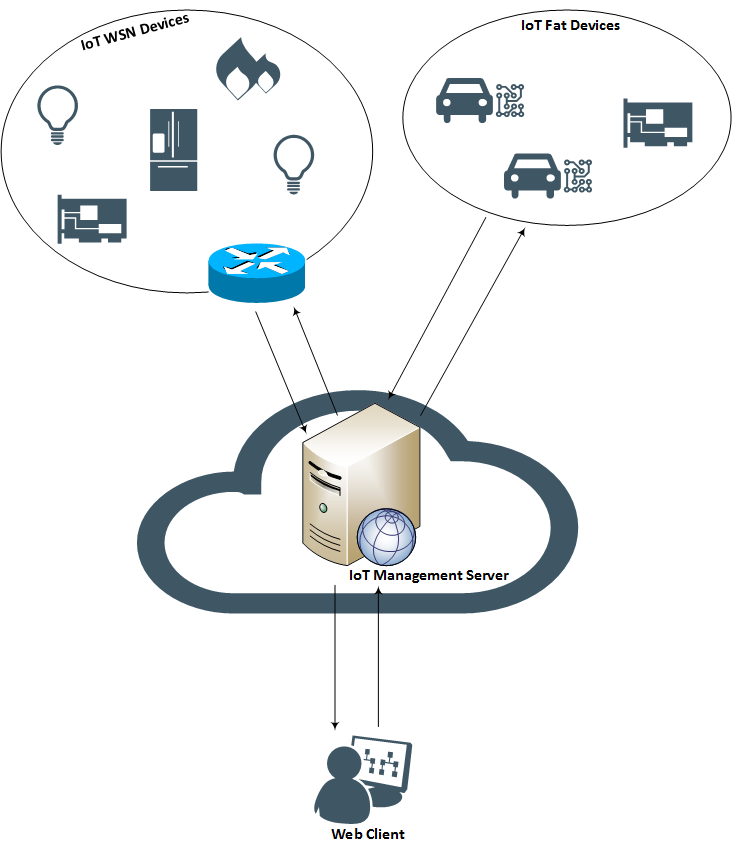
\includegraphics[scale=0.6]{../03_Design/images/systemuebersicht.png}\caption{Systemübersicht}
\end{figure}

\newpage


\begin{landscape}
\section{Klassenstruktur}
\subsection{Klassendiagramm}
\begin{figure}[H]
\centering
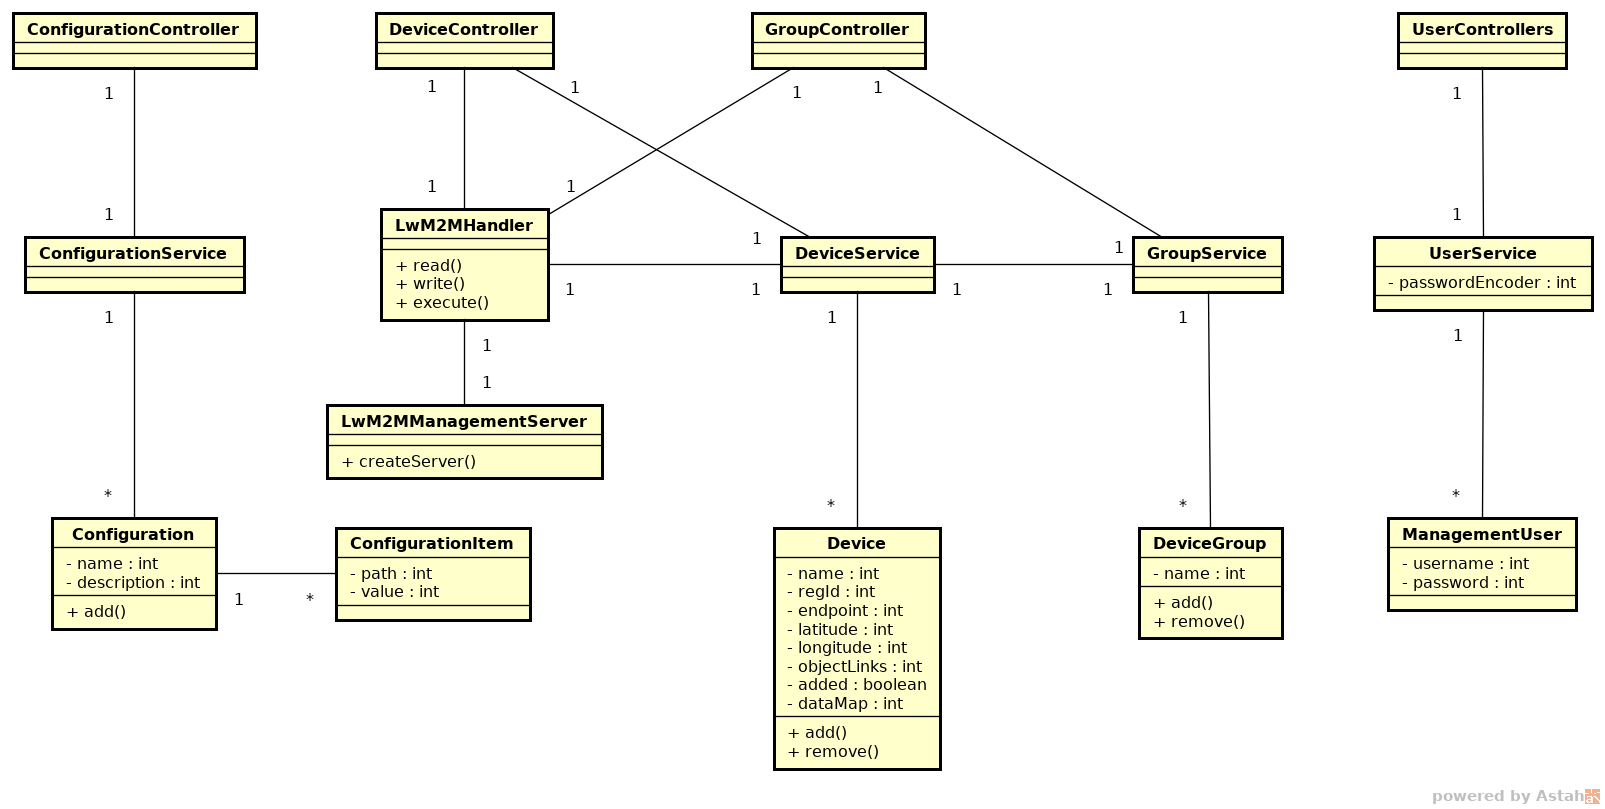
\includegraphics[width=1\textwidth]{../03_Design/images/domainmodel.png}
\caption{Klassendiagramm}
\end{figure}
\end{landscape}

\section{Logische Architektur}
\begin{figure} [H]
	\begin{center}
	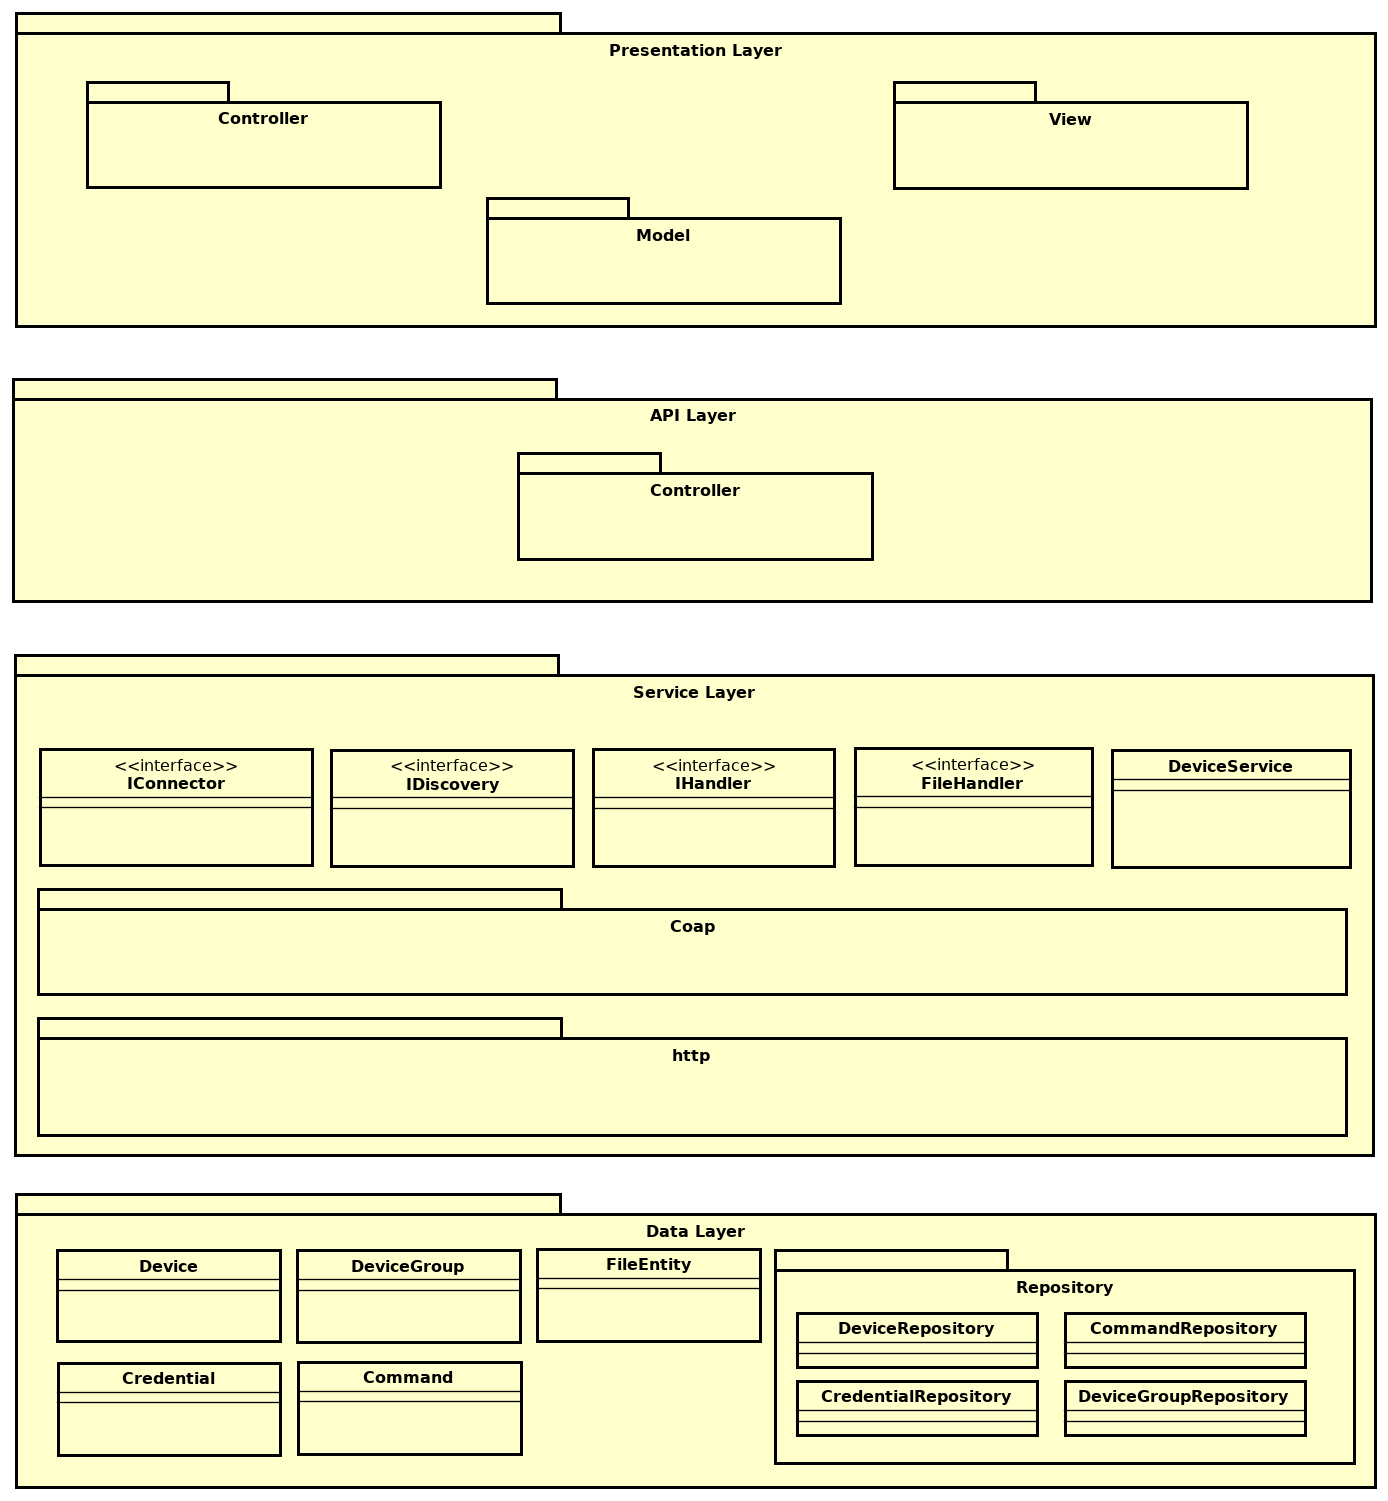
\includegraphics[width=0.90\textwidth]{../03_Design/images/architektur.png}
	\caption{Logische Architektur}
	\end{center}
\end{figure}

\newpage

\subsection{Presentation Layer}


Im Presentation-Layer gibt es Web-Controller und Rest-Controller. Die Web-Controller liefern die HTML-Inhalte aus. Die Rest-Contoller liefern Daten im JSON-Format oder es werden Methoden aus dem Service Layer gestartet, um die Daten zu verarbeiten.


\subsubsection{Packagestruktur}


\begin{table}[H]
\centering
    \begin{tabular}{@{}l p{14.1cm} @{}}\toprule    
    {Packagename} & {Beschreibung}\\ \midrule
    webcontrollers & Alle HTML-Inhalte werden durch die Web-Controller ausgeliefert. Dazu werden die Daten aus dem Service-Layer geholt.\\       
    restcontrollers & Die Rest-Controller führen Methoden auf dem Service-Layer aus und geben die Resultate als JSON zurück an den Client. \\
    \bottomrule
    \end{tabular}
\end{table}

\subsubsection{Klassenstruktur}

\begin{table}[H]
\centering
    \begin{tabular}{@{}l p{11.9cm} @{}}\toprule    
    {Klassenname} & {Beschreibung}\\ \midrule
     FrontWebController & Beinhaltet die Login, Logout und Home Routen.  \\       
     GroupWebController & Liefert alle für Groups relevanten HTML-Inhalte aus. \\       
     DeviceWebController & Liefert alle für Devices HTML-Inhalte aus.  \\       
     DiscoveryWebController & Beinhaltet die Discovery Routen.  \\       
     ConfigurationWebController & Beinhaltet die für die Configuration wichtigen Routen.  \\       
     UserWebController & Liefert die User HTML-Inhalte aus. \\       
     DeviceRestController & Führt Service-Layer Methoden aus und liefert JSON Daten.  \\       
     GroupRestController & Führt Service-Layer Methoden aus und liefert JSON Daten.  \\       
     ConfigurationRestController & Führt Service-Layer Methoden aus und liefert JSON Daten. \\       
     UserRestController & Führt Service-Layer Methoden aus und liefert JSON Daten.  \\         
    \bottomrule
    \end{tabular}
\end{table}

\subsubsection{Schnittstellen}
Der Presentation-Layer hat eine Schnittstelle zum Service-Layer. Alle Daten werden über den Service-Layer geholt und an den Service-Layer gegeben. So ist eine saubere Trennung zwischen Daten und Methoden sichergestellt. 

\newpage

\subsection{Service-Layer}
Der Service-Layer beinhaltet die Klassen, welche für die Verarbeitung der Daten zuständig ist. Hier werden alle Devices erfasst, verbunden und verwaltet. Dazu wird jedes gefundene Device auf der Datenbank hinterlegt. Bei einem Read, Write oder Execute wird das Device aus dem Data Layer geholt und mit den neuen Daten aktualisiert. Dabei wird hier zwischen Applikation-Services und LwM2M-Services unterschieden.

\subsubsection{Packagestruktur}

\begin{table}[H]
\centering
    \begin{tabular}{@{}l p{14.1cm} @{}}\toprule    
    {Packagename} & {Beschreibung}\\ \midrule
    applicationservice & Dieses Package beinhaltet die Klassen, welche die Devices oder Groups erstellen, anpassen usw. \\       
    lwm2mservices & Dieses Package beinhaltet alle Kommunikationsrelevanten Klassen, um mit den Devices Daten auszutauschen. \\
    \bottomrule
    \end{tabular}
\end{table}

\subsubsection{Klassenstruktur}
\begin{table}[H]
\centering
    \begin{tabular}{@{}l p{14.1cm} @{}}\toprule    
    {Klassenname} & {Beschreibung}\\ \midrule
     DeviceService & Holt und speichert die Devices von dem Data-Layer und verarbeitet die Änderungen  \\       
     GroupService & Zugriff auf den Data-Layer. Liest und schreibt alle Groups.  \\       
     ConfigurationService & Zugriff auf den Data-Layer. Liest und schreibt alle Configurationen.  \\  
     UserService & Checkt bei den Logins und verarbeitet die User Schreib- und Lesevorgänge.  \\            
     LocationService & Liest die Locations aus den Devices und gibt sie dem Controller weiter.  \\       
     InfrastructureService & Infrastruktur-Methoden, wie zum Beispiel Server-Uptime.  \\       
     LwM2MHandler & Beinhaltet alle Kommunikation zwischen Devices und dem Management Server.  \\       
     LwM2MManagementServer & Der Server, welche die Befehle aufs Netzwerk schickt und empfängt.  \\       
    \bottomrule
    \end{tabular}
\end{table}
\subsubsection{Schnittstellen}
Der Service-Layer hat eine Schnittstelle zum Data-Layer. Durch den Service-Layer werden die Datenobjekte erstellt, bearbeitet und ausgewertet. Der Presentation-Layer muss immer über den Service-Layer, um eine saubere Abtrennung der Schichten zu gewährleisten.

\newpage

\subsection{Data-Layer}
Der Data-Layer beinhaltet alle Datenobjekte, welche vom laufenden Programm benötigt werden. Diese werden von hier in die Datenbank geschrieben. Das Repository bietet die Datenbankmethoden an, um die Daten in die Datenbank zu speichern.

\subsubsection{Packagestruktur}
\begin{table}[H]
\centering
    \begin{tabular}{@{}l p{14.1cm} @{}}\toprule    
    {Packagename} & {Beschreibung}\\ \midrule
    repositories & Zugriffsmethoden auf die Datenbank. Eigene sowie durch die Library ausgelieferte Methoden. \\       
    \bottomrule
    \end{tabular}
\end{table}

\subsubsection{Klassenstruktur}
\begin{table}[H]
\centering
    \begin{tabular}{@{}l p{14.1cm} @{}}\toprule    
    {Klassenname} & {Beschreibung}\\ \midrule
    Device & Device ist eine Datenklasse, welche alle Daten von einem Device beinhaltet.\\
    DeviceGroup & In der Datenklasse DeviceGroup, werden alle Gruppen verwaltet, damit das Composite-Pattern umgesetzt werden kann.\\
    ManagementUser & Datenklasse für die Loginbenutzer.\\
    Configuration & Configuration Datenklasse, welche eine List von ConfigurationItems beinhaltet. \\
    ConfigurationItem & Datenklasse für die einzelnen ConfigurationItems.\\
    \bottomrule
    \end{tabular}
\end{table}
\subsubsection{Schnittstellen}
Da der Data-Layer die unterste Schicht ist, gibt es nur eine Verbindung zur Datenbank.

\newpage

\section{Komponenten Diagramm}
Die Applikation hat eine typische 3-Tier Architektur. Es wird ein Serverseitiges Templating verwendet. Alle Daten werden daher auf dem Server verarbeitet und als HTML an den Client gesendet. Die Daten werden in einer Datenbank persistiert.
\begin{figure}[H]
\center
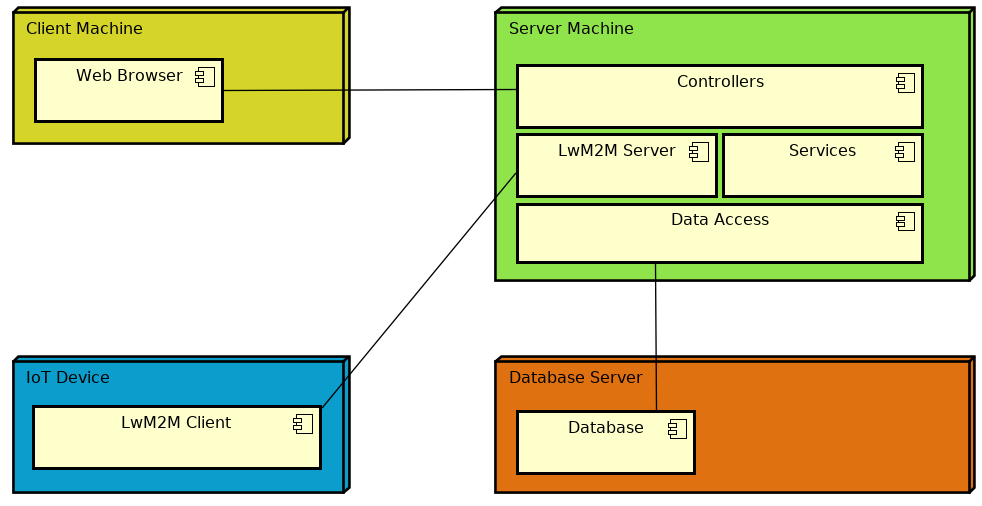
\includegraphics[scale=0.6]{../03_Design/images/architekturuebersicht}\caption{Komponenten Diagramm}
\end{figure}

\section{User Interface Entwurf}
\label{sec:mockups}
\subsection{Design}
Das Projekt erhält eine möglichst einfach gehaltene Benutzeroberfläche. Durch die farbliche Trennung von Funktionen und fixen Bereichen für die Daten, soll die Oberfläche einfach und intuitiv gestaltet werden. Zusätzlich wird die Oberfläche responsiv aufgebaut, damit sie an unterschiedlichen Bildschirmgrössen verwendbar wird.

Es wurden Mock-ups anhand von einfachen Handskizzen erstellt, um das aussehen und die Funktionen der Benutzeroberfläche zu planen.

\subsection{Ansichten}
\subsubsection{Startseite}
\begin{figure} [H]
	\begin{center}
	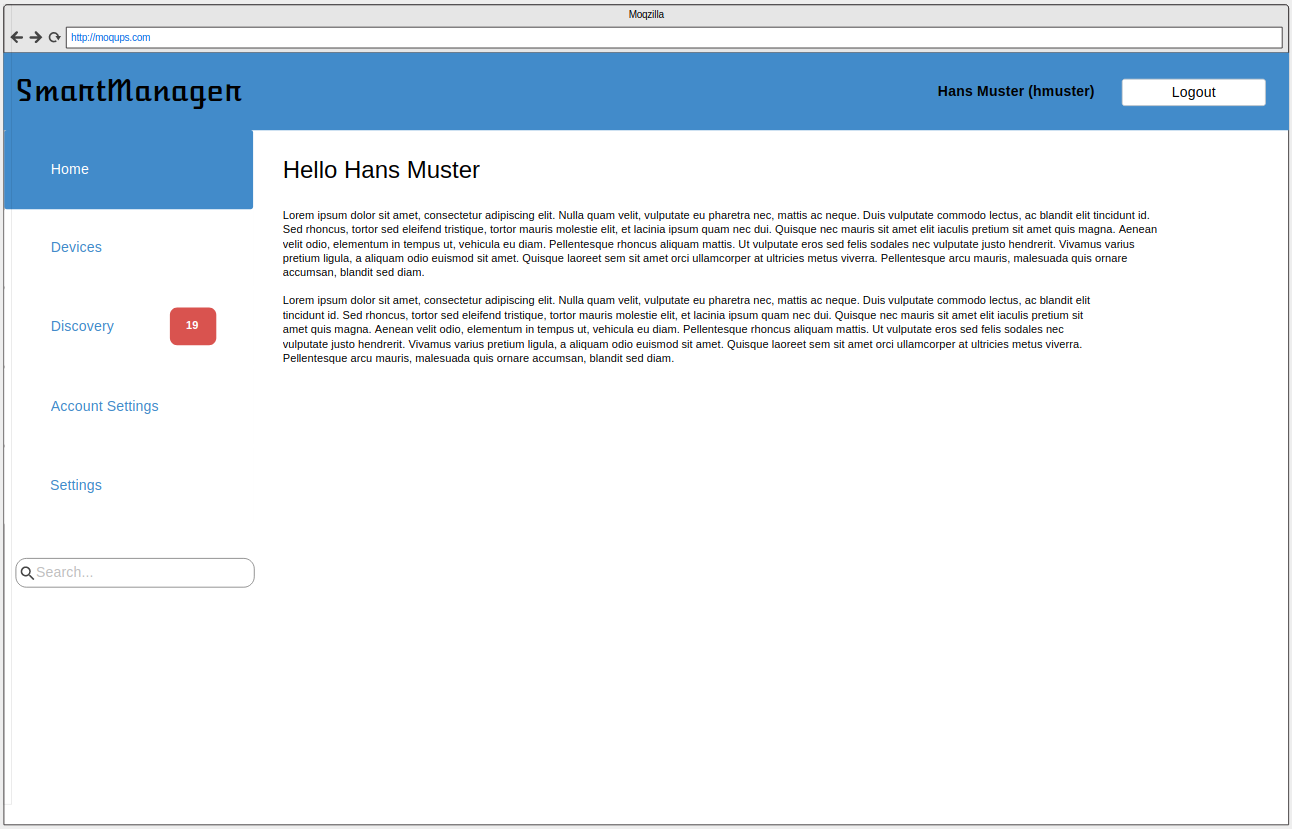
\includegraphics[width=0.80\textwidth]{../03_Design/images/home.png}
	\caption{Startseite}
	\end{center}
\end{figure}
Die Startseite zeigt dem Benutzer Hilfestellungen an und führt den Benutzer durch die ersten Schritte. Auf der Linken Seite befindet sich das Menu und eine Suche. Oben Rechts findet der Benutzer den Loginbereich und die Benutzerangaben.

Beim Menu gibt es statische, sowie dynamische Einträge. Der Discoveryeintrag ist ein dynamischer Eintrag und zeigt die Anzahl gefundenen Geräte an.

\subsubsection{Device List}
\begin{figure} [H]
	\begin{center}
	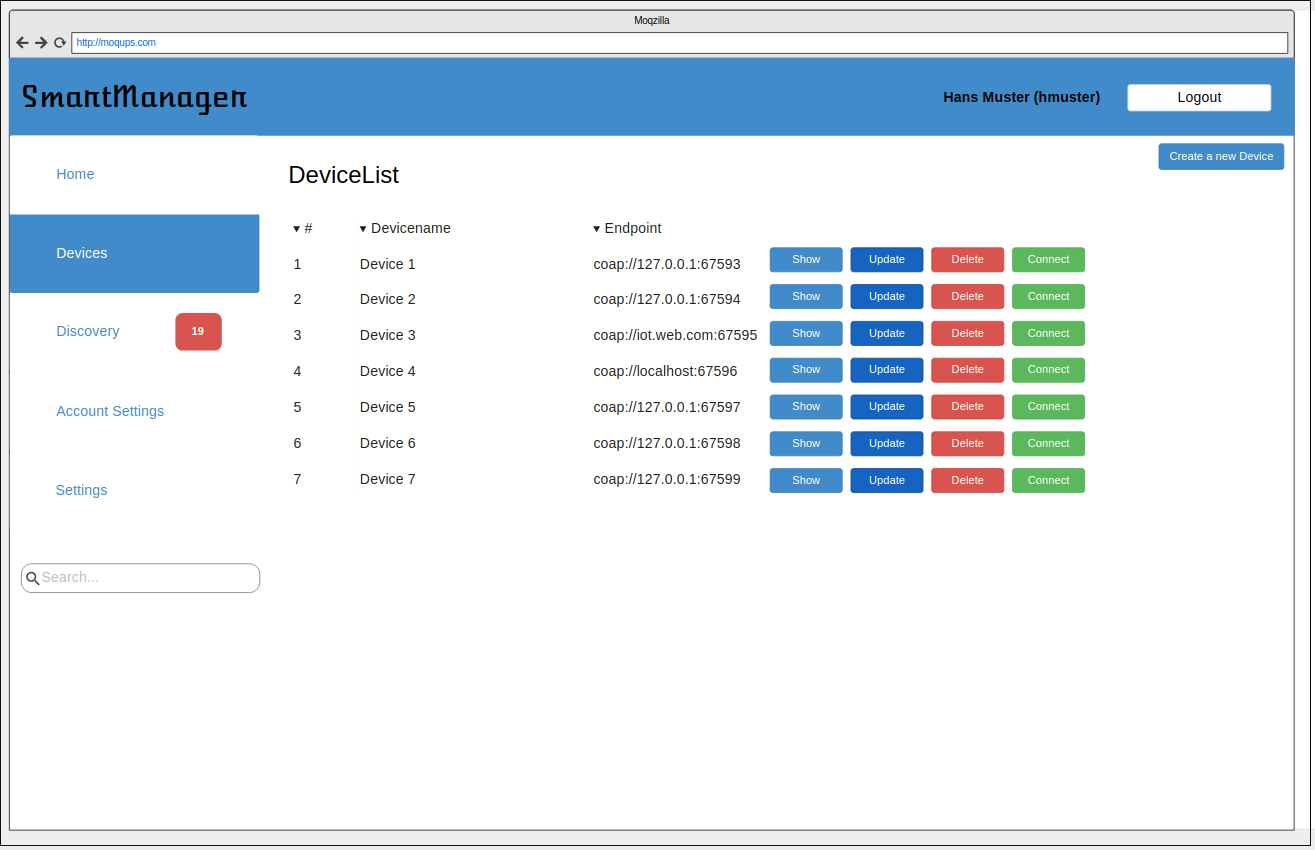
\includegraphics[width=0.80\textwidth]{../03_Design/images/devicelist.png}
	\caption{Device List}
	\end{center}
\end{figure}
In der Device Liste werden alle Devices angezeigt. Dazu wird zu jedem Device die jeweiligen Möglichkeiten als Button eingeblendet. So kann man ein Device betrachten, Anpassen, Löschen und sich mit dem Gerät verbinden. Zusätzlich werden die Daten, wie zum Beispiel Endpoint angezeigt.

Oben rechts befindet sich der Button, um weitere Devices zu erstellen.
\begin{description}
\item [Show] Zeigt die Details zu einem Device an
\item [Update] Führt zum Device Update Formular, damit das Device angepasst werden kann.
\item [Delete] Button, der das Device aus der Applikation löscht
\item [Connect] Button, um sich mit dem Gerät zu verbinden.
\item [Create a new Device] Führt zur Create Device Ansicht.
\end{description}


\subsubsection{Create Device}
\begin{figure} [H]
	\begin{center}
	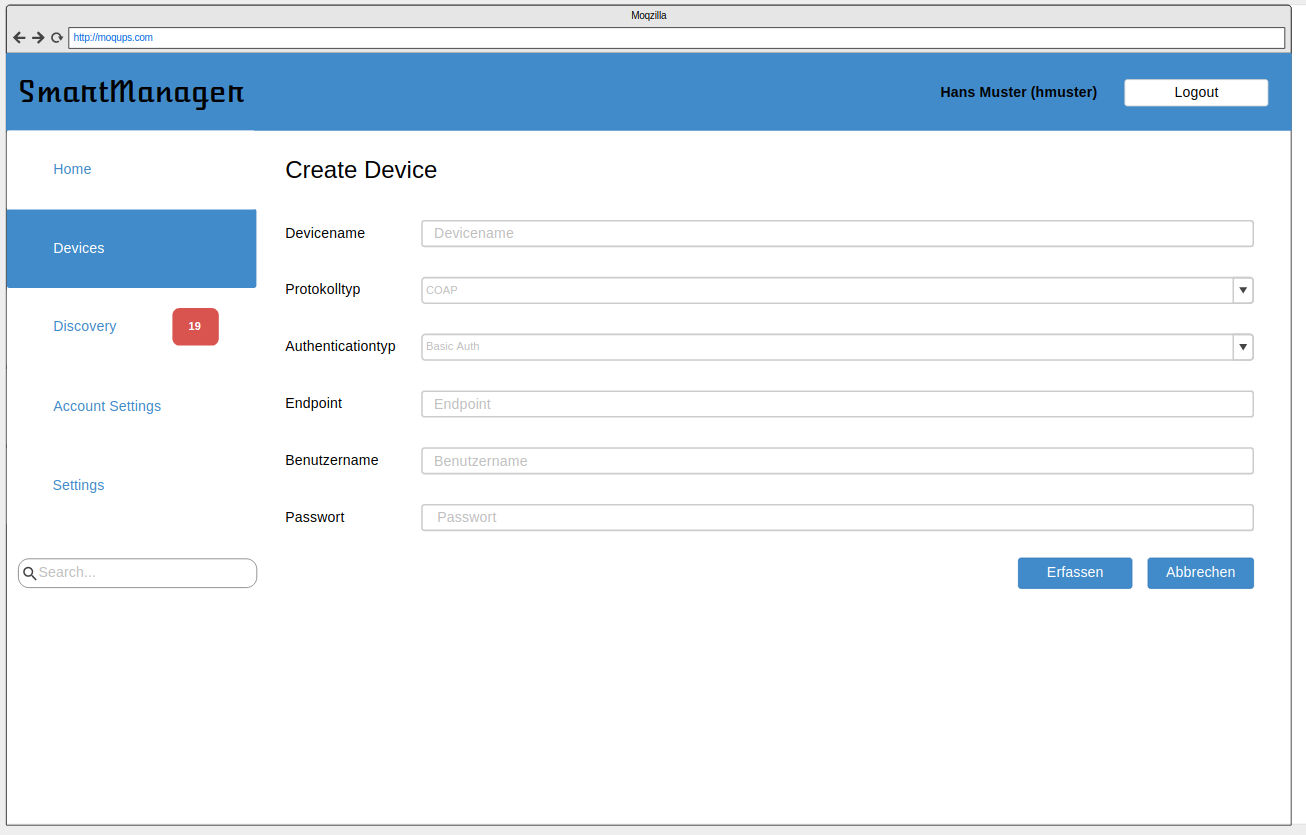
\includegraphics[width=0.80\textwidth]{../03_Design/images/createdevice.png}
	\caption{Create Device}
	\end{center}
\end{figure}
Bei der Create Device Ansicht kann ein neues Device erstellt werden. Dadurch wird das Device manuell erfasst und in der Datenbank abgelegt. Dies kann gemacht werden, wenn das Device nicht via Discovery gefunden worden ist.

Je nach Combobox Auswahl passt sich das Formular an, um zum Beispiel auch Zertifikate hinterlegen zu können.

\begin{description}
\item [Erfassen / Update] Erstellt oder passt ein Device an
\item [Abbrechen] Bricht den Device Create ab und führt zur Device List Ansicht
\end{description}

\subsubsection{Device Details}
\begin{figure} [H]
	\begin{center}
	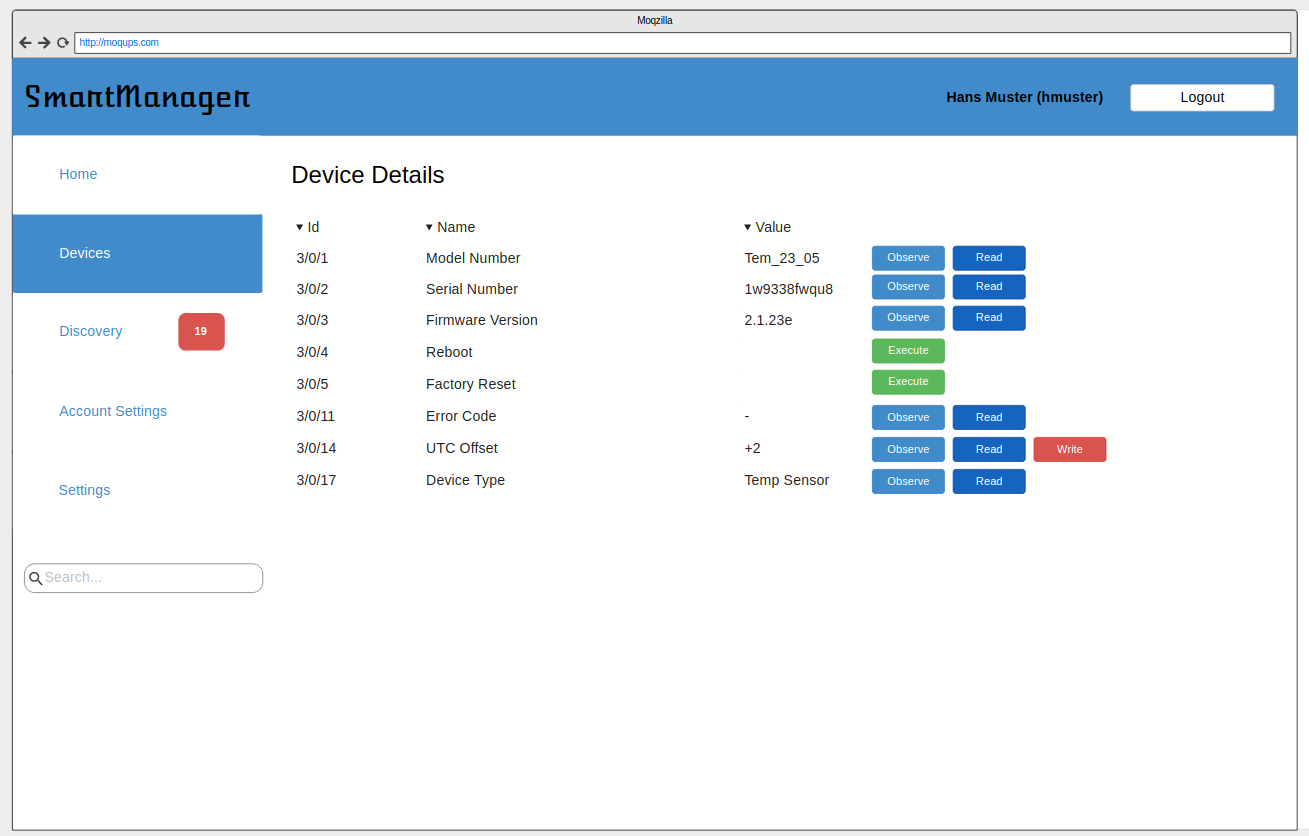
\includegraphics[width=0.80\textwidth]{../03_Design/images/devicedetails.png}
	\caption{Device Details}
	\end{center}
\end{figure}
Alle wichtige Informationen eines Devices werden in dieser Übersicht angezeigt. Zu Jeder Ressource wird die Id, der Name und den aktuellen Wert angezeigt. Je nach Ressource passen sich die Möglichen Aktionen an. Dabei gibt es Observe, Read, Write und Execute. Bei Write wird ein zusätzliches Eingabefeld eingeblendet, um den gewünschten Wert eintragen zu können.

\begin{description}
\item [Observe] Startet ein Observer für die gewünschte Ressource.
\item [Read] Liest die Ressource vom Device
\item [Write] Schreibt den Wert in die Ressource und aktualisiert den Eintrag in der Datenbank
\item [Execute] Führt einen Befehl auf dem Device aus
\end{description}

\subsubsection{Discover Device}
\begin{figure} [H]
	\begin{center}
	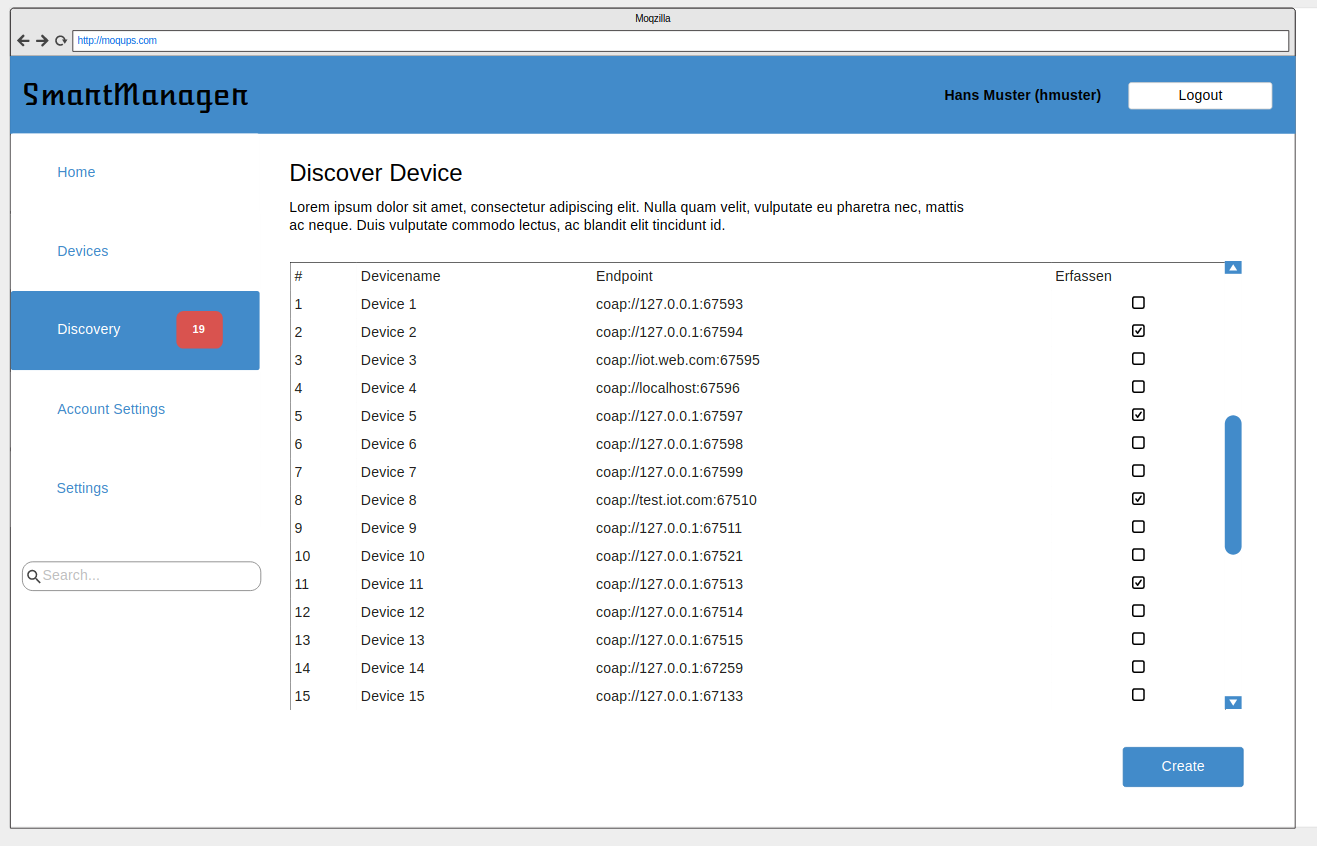
\includegraphics[width=0.80\textwidth]{../03_Design/images/devicediscover.png}
	\caption{Device Details}
	\end{center}
\end{figure}
Alle durch das Discovery gefundenen Devices werden in dieser Übersicht aufgelistet. Dazu werden direkt die wichtigen Daten angezeigt und man hat die Möglichkeit das gewünschte Device zur Applikation hinzuzufügen. Die Anzahl gefundenen Devices werden auf der Linken Seite im Menu angezeigt und passt sich dynamisch an.

\begin{description}
\item [Create] Erstellt für die ausgewählten Devices ein Deviceobjektauf der Datenbank
\end{description}
\chapter{Realisierung}
In diesem Kapitel werden die Realisierungen der Komponenten beschrieben. Es wird versucht, Konzepte und Problemlösungen zu erklären. Vereinzelt werden auch Codeausschnitte gezeigt, sofern diese relevant für das Verständnis sind.

\section{User Interface}
In diesem Abschnitt wird das User Interface gezeigt. Man erhält einen guten Überblick über Funktionalitäten und Aufbau des Front-Ends.

\subsection{Änderungen}
Der erste Prototyp der Applikation wurde gemäss Mock-ups im Kapitel \ref{sec:mockups} erstellt. Beim Requirements- und Architekturreview am 24.04.2017 haben die Teammitglieder unter anderem Änderungen am Erscheinungsbild beschlossen. Durch den Einsatz des LwM2M Servers haben sich auch Anpassungen an der Seitenstruktur ergeben.

Anbei die UI-relevanten Anpassungen:
\begin{itemize}
\item Hauptnavigation von linker Seite an den oberen Bildschirmrand verschoben
\item Entfernen der Accountsettings aus der Hauptnavigation
\item Hinzufügen des Links ''Configurations'' in die Hauptnavigation
\item Verzicht von blauer Farbe am oberen Bildschirmrand, stattdessen schlichteres grau
\item Begrüssungstext am Homebildschirm entfernt, stattdessen Dashboard mit wichtigen Informationen hinzugefügt
\item Hinzufügen einer Navigation für Devices und Gruppen auf der ''Devices'' Seite
\item Das ''Create Device'' Formular wurde entfernt
\item Der ''Observe''-Button unter ''Devices'' wurde entfernt, da diese Funktion nicht implementiert wurde
\item Dem ''Discovery'' wurden Drop-Down Menüs für Konfigurationen und Gruppen hinzugefügt
\end{itemize}

 \newpage

\subsection{Allgemein}
In diesem Unterabschnitt werden die Konzepte erklärt, mit welchen das User Interface realisiert wurde. Das Webinterface wurde HTML, CSS und JavaScript erstellt und als unterstützende Library wurde Twitter Bootstrap verwendet.

\subsubsection{Java Server Pages JSP}
Sämtlicher HTML Code ist in Java Server Pages (JSP) abgelegt. JSP Seiten werden auf dem Server in Java Servlets kompiliert.
\begin{figure}[H]
\centering
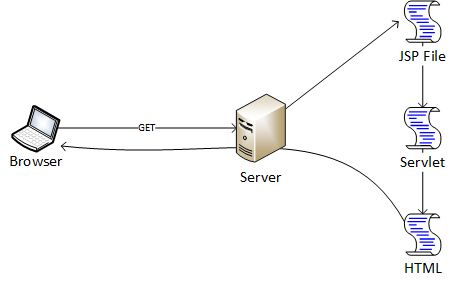
\includegraphics[scale=1]{../04_Realisierung/images/userinterface/jsp.png}
\caption{Java Server Pages}
\end{figure}
Der Client erhält über eine Web-URL vom Server generiertes HTML.

\subsubsection{Java Server Pages Standard Tag Library JSTL}
Mittels JSTL werden in dieser Applikation folgende Aufgaben erfüllt:
\begin{itemize}
\item HTML Fragmente in bestehende Container laden
\item if/else Abfragen für Darstellungen
\item Loop durch Collections im Model für die Darstellung von mehreren Objekten
\end{itemize}

In JSP Seiten wird JSTL mittels folgender Code-Zeile verwendet:
\begin{lstlisting}[language=html5]
<%@ taglib prefix="c" uri="http://java.sun.com/jsp/jstl/core"%>
\end{lstlisting}

Ein Loop durch eine Collection mit Hilfe von JSTP sieht folgendermassen aus:
\begin{lstlisting}[language=html5]
<c:forEach var="collection" items="${collection}">
</c:forEach>
\end{lstlisting}
 \newpage

\subsubsection{Seitenlayout}
Das Seitenlayout ist grundsätzlich sehr einfach. Die Navigation erfolgt am oberen Rand der Seite. Der gesamte Seiteninhalt befindet sich im Content-Bereich. 
\begin{figure}[H]
\centering
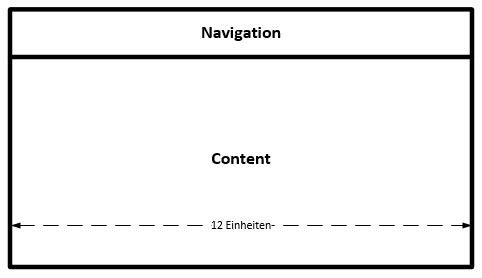
\includegraphics[scale=0.9]{../04_Realisierung/images/userinterface/seitenlayout_allgemein_large.png}
\caption{Seitenlayout Allgemein}
\end{figure}
Das Grid-System von Bootstrap teilt den sichtbaren Bereich in 12 Spalten auf. Jede Spalte besetzt immer $\frac{1}{12}$ der gesamten Fenstergrösse. Bootstrap verwendet folgende CSS Media-Queries für unterschiedliche Bildschirmtypen:
\begin{itemize}
\item Small Devices (min-width: 576px)
\item Tablets (min-width: 768px)
\item Desktops (min-width: 992px)
\item Large Desktops (min-width: 1200px)
\end{itemize}
Sämtlichen div-Containern wird angegeben, wieviele Spalten in welcher Bildschirmgrösse sie besetzen. Mit Bootstrap könnte dies folgendermassen aussehen: 
\begin{lstlisting}[language=html5]
<div class="col-lg-6 col-md-6 col-sm-12 col-xs-12">
</div>
\end{lstlisting}
An diesem Beispiel besetzt dieser Div-Container auf mittelgrossen und grossen Desktops die Hälfte-, auf Tablets und Smartphones die gesamte Bildschirmbreite. Somit wird ein responsives Layout umgesetzt, dass die Applikation sowohl von mobilen-, als auch von Desktop Devices gut nutzbar ist.
 \newpage

\subsubsection{Navigation}
Bootstrap liefert eine ''default-navbar''. Sämtliche Navigationslinks (Home, Device, Discovery, Configurations, User Panel) befinden sich in der Navigationsleiste. Die Navigationsleiste besetzt in jeder Bildschirmgrösse die gesamte Breite.
\begin{lstlisting}[language=html5]
<div class="col-lg-12 col-md-12 col-sm-12 col-xs-12">
</div>
\end{lstlisting}
\begin{figure}[H]
\centering

\includegraphics[scale=0.8]{../04_Realisierung/images/userinterface/navbar_lg.png}
\caption{Navigationsleiste gross}
\end{figure}

Da diese Navigationsleiste auf Smartphones schwierig zu bedienen ist, wird auf der kleinsten Bildschirmgrösse anstatt der normalen Links in der Navigation ein Hamburger-Button verwendet. Anfangs war dieser Button stark umstritten, mittlerweile wird er häufig eingesetzt, weshalb jedem Benutzer klar sein sollte, dass sich dahinter weitere Elemente befinden.
\begin{figure}[H]
\centering
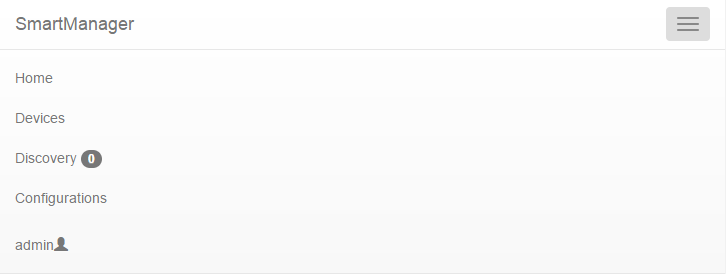
\includegraphics[scale=0.87]{../04_Realisierung/images/userinterface/navbar_xs.png}
\caption{Navigationsleiste xs}
\end{figure}

Die Navigationsleisten sind auf jeder Seite am oberen Bildschirmrand fixiert, sodass bei allfälligem Scrollen die Navigation trotzdem sichtbar bleibt.

Damit duplizierter Code auf jeder Seite verhindert wird, wird der gesamte HTML Code für die Navigation in ein eigenes JSP File ''menuFragment.jsp'' ausgelagert. Der Inhalt des JSP Files wird mittels 
\begin{lstlisting}[language=html5]
<jsp:include page="../../views/menuFragment.jsp" />
\end{lstlisting}
serverseitig ins HTML gerendert.
\subsubsection{Content}
Der gesamte Content Bereich ist auf jeder Seite unterschiedlich gestaltet. Die gesamte Breite von 12 Spalteneinheiten kann verwendet werden.
 \newpage

\subsubsection{Asynchronous JavaScript and XML AJAX}
Damit bei der Kommunikation mit dem Server das User Interface nicht blockiert wird, werden bei sämtlichen Server-Calls AJAX verwendet. AJAX versendet Nachrichten vom Client an den Servern asynchron. Im ''success'' Attribut kann eine Callback-Funktion hinterlegt werden, welche bei erfolgreicher Antwort ausgeführt wird.

In dieser Applikation werden AJAX-Calls nach folgendem Schema ausgeführt:
\begin{lstlisting}[language=js]
$.ajax({
	type : "GET/POST/DELETE",
	url : ctx + "/resource/method",
	success : function() {
		/*some callback code...*/
	},
	error : function(xhr, ajaxOptions, thrownError) {
		window.location.href = ctx + "/";
		alert(thrownError);
	}
});
\end{lstlisting}

Falls der Server mit einem Fehler antwortet, wird die Callback-Funktion im ''error''-Attribut ausgeführt. Der Benutzer wird dabei auf die Haupt-Seite umgeleitet und erhält eine Error-Meldung angezeigt.

\subsubsection{Bootbox}
An verschiedenen Stellen auf der Seite werden Pop-ups benötigt. In diesem Projekt wird die JavaScript Library ''Bootbox'' von Bootboxjs.com verwendet.

\begin{figure}[H]
\centering
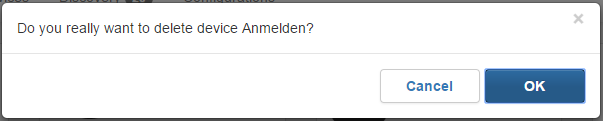
\includegraphics[scale=0.9]{../04_Realisierung/images/userinterface/bootbox.png}
\caption{Bootbox}
\end{figure}

Der JavaScript Code für die Erstellung und Verwendung der Bootbox ist leicht verständlich.

\begin{lstlisting}[language=js]
bootbox.confirm({
	size : "large",
	title : "some title",
	message : content,
	callback : function(ok) {
		if (ok) {
			/*save, redirect etc.*/		
		}
	}
});
\end{lstlisting} 

Als ''message''-Attribut kann ein String oder auch HTML Code eingefügt werden.  Beim ''Callback''-Attribut kann eine Callback-Funktion hinterlegt werden. Diese wird ausgeführt, wenn das Pop-up Fenster geschlossen wird. Die if-Abfrage stellt sicher, dass der darinliegende Code nur ausgeführt wird, wenn ''OK'' auf geklickt wird.
 \newpage


\subsubsection{Google Maps API}
An verschiedenen Stellen auf der Seite werden Devices auf Google Maps Karten angezeigt. Dies gibt dem Benutzer eine schnelle Übersicht der Lokalitäten der IoT-Devices.

Über die JavaScript-Funktion ''initMap()'' wird die (leere) Map geladen. Danach werden über die Funktion ''getLocations()'' die Locations der benötigten IoT-Devices vom Server abgefragt. Über die ''insertLocations()''-Funktion werden die Punkte auf der Map eingezeichnet.

\subsection{Home}
Die Home-Seite dient als Einstiegspunkt und Übersichtsseite. Dem Benutzer sollen Informationen über die Applikation und die verwaltete Infrastruktur angezeigt werden.

\begin{figure}[H]
\centering
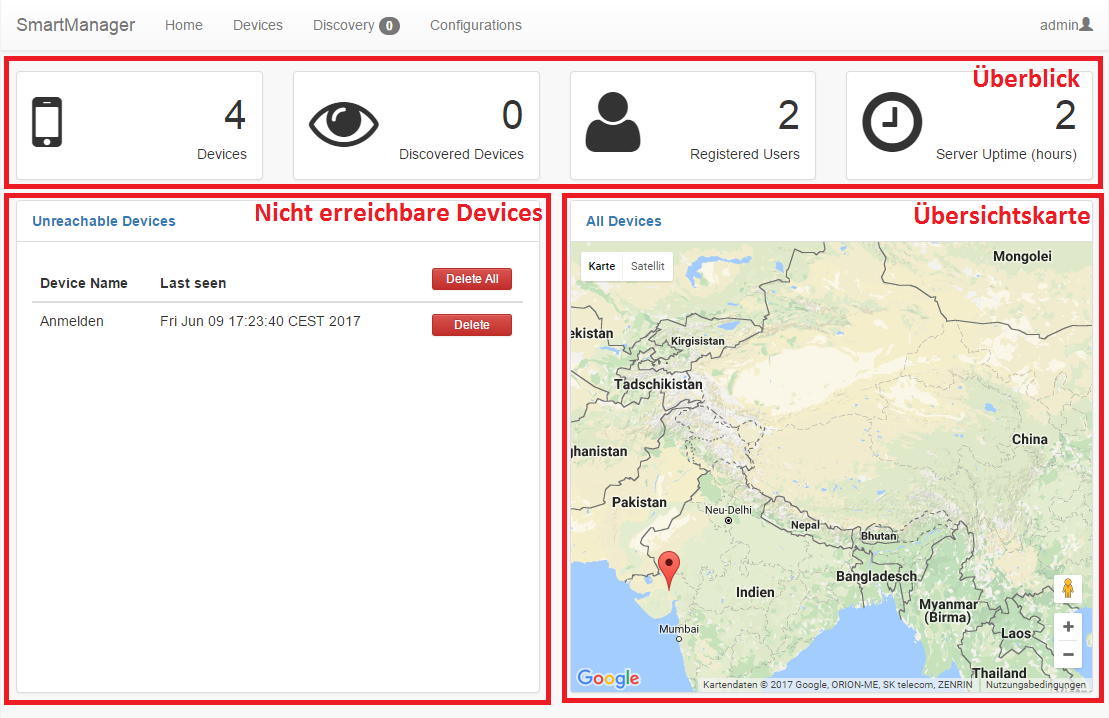
\includegraphics[scale=0.57]{../04_Realisierung/images/userinterface/home.png}
\caption{Dashboard}
\end{figure}

\subsubsection{Überblick}
In diesem Bereich werden dem Benutzer folgende vier Informationen auf den ersten Blick angezeigt:
\begin{itemize}
\item Gesamtanzahl erfasster Devices im System
\item Anzahl Devices im Discovery (noch nicht verwaltet)
\item Anzahl registrierter Benutzer
\item Server Uptime in Stunden
\end{itemize}
 \newpage

\subsubsection{Nicht erreichbare Devices}
Sind Devices nicht mehr erreichbar, muss dies dem Benutzer mitgeteilt werden. Hat sich ein Device mehr als 30 Minuten nicht mehr beim Server gemeldet, so erscheint es in dieser Tabelle. Klickt der Benutzer auf ''Delete'' respektive ''Delete All'', so werden die JavaScript Funktionen ''deleteUnreachableDevice(id, name)'' und ''deleteAllUnreachableDevices()'' ausgeführt. Über eine AJAX-Anfrage werden die entsprechenden Serverpfade aufgerufen.

\subsubsection{Übersichtskarte}
Auf dieser Übersichtskarte werden alle im Device gespeicherten Locations von IoT-Devices angezeigt.

\newpage
\subsection{Discovery}
Auf der Discovery Seite sieht der Benutzer alle registrierten Devices. Sämtliche Devices registrieren sich am LwM2M Server. Sind sie vom Benutzer noch nicht hinzugefügt worden, so erscheinen sie auf dieser Seite.

\begin{figure}[H]
\centering
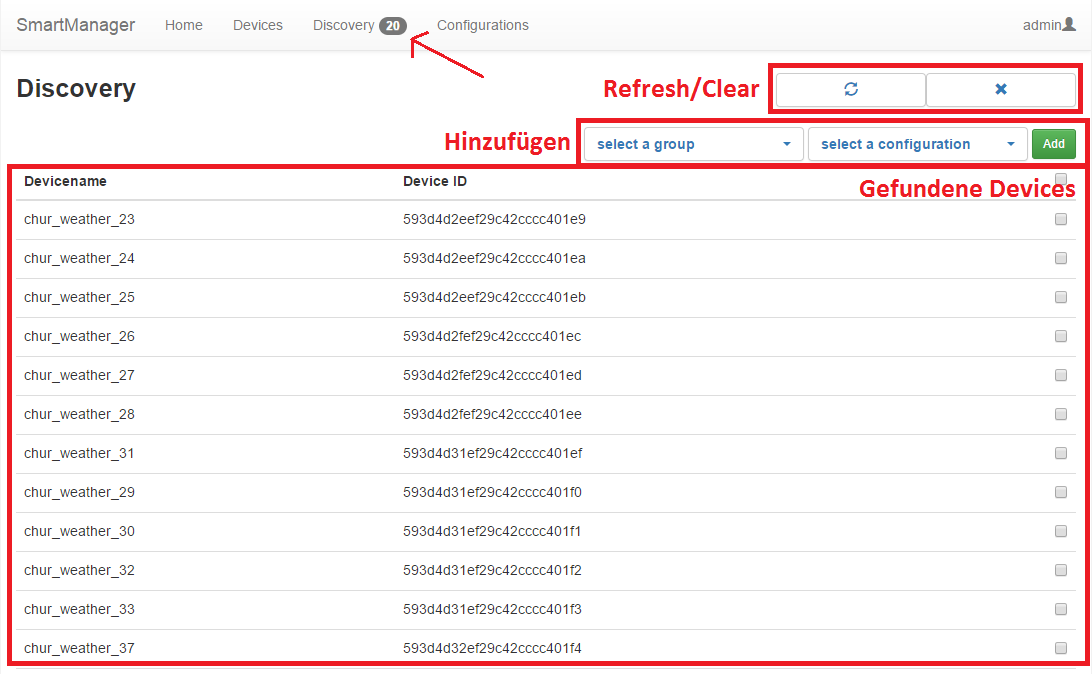
\includegraphics[scale=0.57]{../04_Realisierung/images/userinterface/discovery.png}
\caption{Discovery}
\end{figure}

\subsubsection{Gefundene Devices}
Ist ein Device vom Benutzer noch nicht hinzugefügt worden, besitzt das Attribut ''added'' den Wert ''false''. Nachdem der Benutzer das Device hinzugefügt hat, wird dem Device das Attribut ''added'' auf ''true'' gesetzt und erscheint deshalb nicht mehr.

\subsubsection{Hinzufügen}
Beim ''Add''-Button werden die selektierten Devices hinzugefügt. Es besteht die Möglichkeit, beim Hinzufügen eine Gruppe oder eine Initiale Konfiguration zu setzen.

\begin{figure}[H]
\centering
\includegraphics[scale=0.57]{../04_Realisierung/images/userinterface/discovery_addgroup.png}
\caption{Discovery Gruppenauswahl}
\end{figure}

Die selektierten Werte in den Drop-Down-Listen werden dem Server beim Hinzufügen des Devices übergeben.

\subsubsection{Refresh/Clear}
Mit dem Refresh Button wird die Seite neu geladen, damit frisch registrierte Devices angezeigt werden. Der Clear Button leert die Liste von Devices. Melden sich die Devices zu einem späteren Zeitpunkt nochmals, so tauchen sie in dieser Ansicht wieder auf.
 \newpage

\subsection{Configuration}
Benutzer können auf dieser Seite eigene Konfigurationen erstellen. Sämtliche schreibbaren LwM2M-Objekte können gesetzt werden. Nach der Erstellung einer Konfiguration kann sie auf neue Devices oder eine Devicegruppe geschrieben werden.

\begin{figure}[H]
\centering
\includegraphics[scale=0.57]{../04_Realisierung/images/userinterface/config_overview.png}
\caption{Configuration Übersicht}
\end{figure}

\subsubsection{Konfigurationslisten}
Sämtliche erstellten Konfigurationen werden hier aufgelistet. Eine Konfiguration kann einzeln gelöscht und editiert werden.
 \newpage

\subsubsection{Neue Konfiguration}
Mit dem ''create new configuration'' Button öffnet sich ein neues Pop-up, in welchem der Benutzer eine neue Konfiguration erstellt.

\begin{figure}[H]
\centering
\includegraphics[scale=0.6]{../04_Realisierung/images/userinterface/config.png}
\caption{Configuration Neu}
\end{figure}
Sowohl Name, als auch Description können frei gewählt werden. Beim selektieren der Object ID (linkes Drop-Down Menü) wird eine Ajax Anfrage an den Server gesendet. Als Antwort erhält man informationen über die beiden anderen Felder. Sind Multi-Instanzen nicht erlaubt, so bleibt das Zahlenfeld ausgegraut, die Daten für das rechte Drop-Down werden dynamisch gerendert, sind also abhängig von der links gewählten Object-ID. Das Value Feld kann frei beschrieben werden. Serverseitig werden Überprüfungen des Typs, sowie Character Escaping durchgeführt.

Nachdem der Benutzer den Plus-Button geklickt hat, erscheinen Object Link und Value als Configuration Item in einer Liste und es kann mit weiteren Einstellungen forgefahren werden. Sobald der Benutzer ''Save'' drückt, wird clientseitig ein JSON-formatiertes Konfigurationsobject erstellt und an den Server gesendet.

\begin{lstlisting}[language=json]
[
  "Config_Chur_Temperatur_1", 
  "Dies ist eine Beispielkonfiguration fuer Temperatursensoren", 
  {
	"Object Link": "3305/0/5806",
	"Value": "5.5382"
  }, 
  {
	"Object Link": "3201/0/5750",
	"Value": "I/O"
  }
]
\end{lstlisting}



\subsection{Devices und Groups}
Benutzer können auf dieser Seite einzelne Devices und Gruppen verwalten. Sie ist also sozusagen das Kernstück der Applikation, da viele Use-Cases in diesem Bereich abgedeckt werden.

\begin{figure}[H]
\centering
\includegraphics[scale=0.57]{../04_Realisierung/images/userinterface/devices_start.png}
\caption{Devices}
\end{figure}

\subsubsection{Komponentenverwaltung}
Der Bereich der Komponentenverwaltung ist zu Beginn leer. Der Benutzer muss zuerst eine Gruppe oder ein Device selektieren, damit der entsprechende Inhalt geladen wird. Es gibt zwei verschiedene Komponentenverwaltungen, die Device- und die Gruppenverwaltung. Nachdem im Navigationsbereich link eine Gruppe/Device gewählt wurde, wird vom Server ein HTML Fragment angefordert und dargestellt.
 \newpage

\subsubsection{Navigationsbaum}
Auf der linken Seite befindet sich der Navigationsbaum. Darin befinden sich sämtliche Gruppen und Devices hierarchisch angeordnet. 

\begin{figure}[H]
\centering
\includegraphics[scale=0.84]{../04_Realisierung/images/userinterface/componentstree.png}
\caption{Komponentenbaum}
\end{figure}

Gruppen dürfen beliebig tief verschachtelt werden, sind jedoch einzigartig und haben höchstens eine direkte Elterngruppe. Es dürfen beliebig viele Root Gruppen bestehen. Diese erscheinen in der Navigation zuoberst (ohne aufklappen zu müssen), ansosten unterscheiden sie sich nicht von ''normalen'' Gruppen. 

Devices entsprechen den Blattknoten, sie dürfen keine Kindsknoten enthalten. Devices dürfen aber bei beliebig vielen Gruppen als Kindsknoten existieren, somit hat der Benutzer maximale Freiheiten beim Verwalten seiner Devices.

Der Navigationsbaum wurde mit Hilfe der gijgo Library implementiert. Gijgo ist eine JavaScript (jQuery) Library, welche aus Baumstrukturen aufklappbare Navigationen erstellt.

\begin{lstlisting}[language=js]
$('#tree').tree(
	{
		primaryKey : 'id',
		uiLibrary : 'bootstrap',
		dataSource : ctx + '/groups/getAll'
	});
\end{lstlisting}

Die Verwendung der Library ist sehr simpel. Auf einem selektierten Div-Container kann die Funktion tree() ausgeführt werden. Als Datenquelle wird eine URL angegeben. Diese API liefert die Baumstruktur im JSON Format, welche von der Gijgo-Library direkt interpretiert wird.
 \newpage

Anbei ist ein einfaches Beispiel einer Komponentenhierarchie.

\begin{lstlisting}[language=json]
[
	{
		"id": "groups/593e584eed204e174c2a0cc4",
		"text": "ZH",
		"children": 
	  	[
		  	{
				"id": "devices/593e5845ed204e174c2a0cae",
				"text": "chur_weather_23"
			},
			{
				"id": "devices/593e5845ed204e174c2a0caf",
				"text": "chur_weather_24"
			}
		]
	}
]
\end{lstlisting}
 \newpage

\subsection{Devices}
Wählt man in der Navigation ein Device an, so wird eine Anfrage für das HTML Fragment für Devices gestartet. 

\begin{figure}[H]
\centering
\includegraphics[scale=0.57]{../04_Realisierung/images/userinterface/devicefragment_collapsed.png}
\caption{Übersicht einzelnes Device}
\end{figure}

\subsubsection{Aktionen}
Mit ''Delete Device'' wird das Device komplett von der Datenbank entfernt. Mit ''Group Memberships'' kann das Device unterschiedlichen Gruppen zugewiesen werden. ''Read All'' führt ein Lesevorgang über sämtliche verfügbaren Objekte (siehe weiter unten).

\subsubsection{Allgemeine Informationen}
Im Bereich der allgemeinen Informationen erhält der Benutzer nützliche Device-Details angezeigt, ebenfalls wird mittels Google Maps API die Location des Devices automatisch angezeigt.
\newpage
\subsubsection{Deviceobjekte}
Die Deviceobjekte sind standardmässig zugeklappt. Die einzelnen Objekte sind jeweils eine aufklappbare Panels. Bei der Registration meldet ein Device dem LwM2M Server, welche Objekte es unterstützt. Die Panels werden, abhängig der unterstützten Objekte, dynamisch erzeugt. Mit dem ''Read Multiple'' Button werden sämtliche Felder des Objekts gelesen.

\begin{figure}[H]
\centering
\includegraphics[scale=0.57]{../04_Realisierung/images/userinterface/devicefragment.png}
\caption{Anzeige Objektdetails}
\end{figure}

Sobald der Benutzer ein Panel anklickt, werden die darunterliegenden Attribute in einer dynamisch generierten Tabelle angezeigt. Zu Beginn sind noch keine Werte vorhanden. Es muss entweder pro Feld einzeln-, oder über den ''Read Multile''- respektive ''Read All''-Button vom Device gelesen werden.

Auf der rechten Seite werden Buttons für die unterstützen Aktionen angezeigt. Jede Instance ID hat in der XML-Spezifikation hinterlegt, welche Aktionen verfügbar sind.

\begin{figure}[H]
\centering
\includegraphics[scale=0.7]{../04_Realisierung/images/userinterface/rwe.png}
\caption{RWE Buttons}
\end{figure}
\newpage

\subsection{Groups}
In der Gruppenansicht stehen dem Benutzer viele Funktionen für die Verwaltung von Devices und Groups zur Verfügung. In der Map-Übersicht sind alle Devices ersichtlich.

\begin{figure}[H]
\centering
\includegraphics[scale=0.57]{../04_Realisierung/images/userinterface/groups.png}
\caption{Gruppenansicht}
\end{figure}
\newpage

\subsubsection{Group Members}
Gruppenmitglieder können unter ''Group Members'' verwaltet werden. 

\begin{figure}[H]
\centering
\includegraphics[scale=0.8]{../04_Realisierung/images/userinterface/groupmembers.png}
\caption{Gruppenmitglieder}
\end{figure}

Sowohl Devices, als auch Gruppen werden auf der linken Seite angezeigt, diese können hinzugefügt werden. Die Liste wird mittels Ajax-Anfrage vom Server abgerufen. Es wird ein Delta zwischen der Menge aller Komponenten und den aktuellen Mitgliedern erstellt.

Auf der rechten Seite sind die Mitglieder aufgelistet, sobald ''OK'' gedrückt wird, wird eine Liste mit den angepassten Mitgliedern an den Server gesendet.

Diese Verwaltung wurde mit Hilfe der Bootstrap-Duallist-Box Library implementiert. 
\subsubsection{Group Memberships}
Die Mitgliedschaft der Gruppe wird über diesen Button verwaltet. Eine Gruppe kann nur über eine Gruppenzugehörigkeit gleichzeitig verfügen. Die Mitgliedschafsverwaltung wird ebenfalls über die Bootstrap-Duallist-Box Library implementiert.

\subsubsection{Add New Child Group}
Mit dieser Funktion kann der Gruppe eine neue Kindsgruppe hinzugefügt werden. Serverseitig wird überprüft, ob der Gruppenname bereits existiert.\\
\newpage

\subsubsection{Write Configuration}
Zuvor erstellte Konfigurationen können auf Gruppenebene verteilt werden. Alle definierten Schreiboperationen werden auf alle Nachfahren verteilt. Nach erfolgter Konfiguration erhält der Benutzer eine Response vom Server und wird über den Erfolg der Schreiboperationen benachrichtigt. Die Response wird auf dem Server generiert und dem Client im HTML Format ausgeliefert.

\begin{figure}[H]
\centering
\includegraphics[scale=0.6]{../04_Realisierung/images/userinterface/configresults.png}
\caption{Konfigurationsantwort}
\end{figure}
\newpage

\subsubsection{Execute}
Execute Funktionen wie beispielsweise einen Neustart können auf Gruppenebene ausgeführt werden. Betroffen sind sämtliche Nachfahren der Gruppe. Execute Funktionen definieren sich in den XML-Models mit der Operation ''E''.

\begin{figure}[H]
\centering
\includegraphics[scale=0.6]{../04_Realisierung/images/userinterface/execute.png}
\caption{Execute}
\end{figure}

Nach der Auswahl des linken Felds (Object ID) wird eine Anfrage an den Server gesendet. Das mittlere und das rechte Feld werden aufgrund der Response vom Server dynamisch generiert.

\subsubsection{Write}
Die Write Funktion ist identisch zu der Write Configuration Funktion, mit dem einzigen Unterschied, nur ein Konfigurationselement zu senden. Es muss somit nicht eine Konfiguration erstellt werden, der zu beschreibende Wert kann direkt definiert werden.
\newpage

\subsection{User Management}
In der Benutzerverwaltung kann der eingeloggte User Änderungen an benutzerspezifischen Attributen vornehmen. Momentan kann der Administrator lediglich neue Benutzer hinzufügen und bestehende Benutzer löschen. Änderungen am Passwort können alle Benutzer vornehmen. 

\begin{figure}[H]
\centering
\includegraphics[scale=0.6]{../04_Realisierung/images/userinterface/usermanagement.png}
\caption{Benutzerverwaltung Admin}
\end{figure}

\newpage

\section{Controllers}
In diesem Abschnitt wird die Implementiert der einzelnen Controller beschrieben sowie eine Erklärung der verwendeten Spring Funktionen.

\subsection{Allgemein}
Mit den Controllern werden alle Routen und Web API Methoden definiert. Für dies wurde das Spring Framework mit der spring-webmvc (v4.3.7) und der spring-web (v4.3.7) Library verwendet. Das Spring Framework hat dabei viel Arbeit abgenommen und den grossen Teil bereits implementiert. Im Controller wurden daher nur noch die Daten aus dem Service-Layer geholt, mit der View verbunden und an den Client zurückgesendet.

\subsection{Verwendete Annotations}
\subsubsection{@Controller}
Die @Controller Annotation ist die Spring Bezeichnung für einen Web Controller. Diese Annotation wird direkt über dem Klassennamen platziert. Hier sieht man das Beispiel des DeviceWebController:
\begin{lstlisting}[language=java]
@Controller
@RequestMapping("/devices")
public class DeviceWebController {
...
}
\end{lstlisting}

Der Controller führt die zur Route passende Methoden aus, holt die Daten aus dem Service Layer und mappt diese auf das Model und gibt die View mit den Daten zurück. Dabei ist der Rückgabe immer der Name der View und wird als String an das Spring Framework übergeben.

Dies ist ein Beispiel von der /groups/id Route. Als ersten Schritt wird die Gruppe aus dem Service-Layer geholt und dem Model hinzugefügt. Danach gibt man im Return-Wert die gewünschte View-Datei an. Hier im Beispiel ist dies die groupFragment.jsp Datei. Der ganze Rest wird durch Spring und der Template Engine erledigt.
\begin{lstlisting}[language=java]
@RequestMapping(value = "/{id}", method = RequestMethod.GET)
public String showGroupDetails(Model model, @PathVariable("id") String id) {
	model.addAttribute("group", groupService.getGroup(id));
	return "devices/groupFragment";
}
\end{lstlisting}
\newpage

\subsubsection{@RestController}
Die zweite Controllerart ist der RestController. Auch diese Annotation wird direkt oberhalb des Klassennamens platziert. Im gegensatz zur @Controller Annotation gibt der RestController Daten im JSON-Format zurück. 

Die Rückgabewerte werden von Spring automatisch in das JSON-Format umgewandelt und an den Client gesendet. Dies setzt voraus, dass der Rückgabetyp entweder eine get-Methode auf alle Felder besitzt oder ein einfacher Datentyp wie zum Beispiel String ist.
Hier sieht man, wie eine Restmethode aussehen könnte. Es werden alle Gruppen aus dem Service-Layer geholt und als JSON an den Client gesendet.
\begin{lstlisting}[language=java]
@RequestMapping(value = "/list", method = RequestMethod.GET)
public List<DeviceGroup> getGroupList() {
	return groupService.getAllGroups();
}
\end{lstlisting}

Das durch Spring generierte JSON sieht wie folgt aus:
\begin{lstlisting}[language=json]
[
    {
        "id": "593e57293f56e959e84339f9",
        "name": "_unassigned",
        "children": []
    },
    {
        "id": "593e828a3f56e96a8b665fa8",
        "name": "CH",
        "children": [
            {
                "id": "593e82903f56e96a8b665fa9",
                "name": "Luzern",
                "children": []
            }
        ]
    },
    {
        "id": "593e82903f56e96a8b665fa9",
        "name": "Luzern",
        "children": []
    }
]
\end{lstlisting}

\subsubsection{@RequestMapping}
Durch das RequestMapping gibt man die Route und die Methode an, auf welche der Controller reagieren soll. Diese Annotation kann bei der Klasse, sowie bei jeder Methode angegeben werden. Gibt man das RequestMapping bei der Klasse an, gilt dieses für alle weiteren Methoden in der Klasse.

Hier sieht man wie die Route /users/delete mit der Requestmethode POST definiert wird. Durch diese zwei Annotationen weiss Spring, dass diese Methode ausgeführt werden muss.
\begin{lstlisting}[language=java]
@RestController
@RequestMapping("/users")
public class UserRestController {

	@RequestMapping(value = "/delete", method = RequestMethod.POST)
	public String deleteUser(@RequestParam("username") String username) {}
	...
}
\end{lstlisting}
\subsubsection{@PathVariable}
Um einer Route eine Pfadvariable zu hinterlegen, gibt es die PathVariable Annotation. Diese wird in der Parameterliste der Methode eingefügt, um die Werte aus der Route zu erhalten.

In diesem Beispiel wurde eine Pfadvariable Id definiert. Dies geschieht durch die geschweiften Klammern. Um die Variable in der Methode benutzen zu können, wird die @PathVariable eingefügt. Dadurch nimmt Spring den Id-Teil der Route und wandelt es in diesem Beispiel zu einem String um. So kann man die Variable in der gesamtem Methode verwenden.
\begin{lstlisting}[language=java]
@RequestMapping(value = "/{id}/delete", method = RequestMethod.DELETE)
public void removeGroup(@PathVariable("id") String id) {
	groupService.deleteGroup(id);
}
\end{lstlisting}
\subsubsection{@RequestParam}
Um Request Parameter abzufangen, gibt es die @RequestParam Annotation. Durch diese können zum Beispiel Formulardaten abgefangen werden und der Methode zur Verfügung gestellt werden. Dazu werden alle zu erwarteten Request Parameter als Variable in der Parameterliste der Methode an.

In diesem Beispiel wird eine List von Strings übergeben. Der Post muss den Parameter auch value nennen, damit Spring dies richtig erkennt. Wird alles korrekt übergeben, wandelt Spring die erhaltenen JSON-Daten in das gewünschte Format um.
\begin{lstlisting}[language=java]
@RequestMapping(value = "/{id}/removeFromGroups", method = RequestMethod.POST)
public void removeFromGroups(@PathVariable("id") String id, @RequestParam("value") List<String> value) {
	groupService.removeDeviceFromGroups(value, id);
}
\end{lstlisting}
\newpage

\subsection{Übersicht aller Routen}
\begin{longtable}{ p{11cm} p{4cm} l}
\hline 
\multicolumn{1}{p{11cm}}{\textbf{URI}} & 
\multicolumn{1}{p{4cm}}{\textbf{Method}} &  \\ \hline 
\endfirsthead

\hline 
\multicolumn{1}{p{11cm}}{\textbf{URI}} & 
\multicolumn{1}{p{4cm}}{\textbf{Method}} &  \\ \hline 
\endhead

/	&	GET	 \\ \addlinespace
/login	&	GET	 \\ \addlinespace
/logout	&	GET	 \\ \addlinespace
/users	&	POST	 \\ \addlinespace
/users/add	&	POST	 \\ \addlinespace
/users/delete	&	POST	 \\ \addlinespace
/users/checkUser	&	POST	 \\ \addlinespace
/users/userAddFragment	&	GET	 \\ \addlinespace
/users/userDeleteFragment	&	GET	 \\ \addlinespace
/users/userEditFragment	&	GET	 \\ \addlinespace
/users/{id}/edit	&	POST	 \\ \addlinespace
/discovery	&	GET	 \\ \addlinespace
/discovery/clean	&	GET	 \\ \addlinespace
/configurations	&	GET	 \\ \addlinespace
/configurations/add	&	POST	 \\ \addlinespace
/configurations/createConfigurationFragment	&	GET	 \\ \addlinespace
/configurations/delete	&	POST	 \\ \addlinespace
/configurations/{id}/editConfigurationFragment	&	GET	 \\ \addlinespace
/devices	&	GET	 \\ \addlinespace
/devices/add	&	POST	 \\ \addlinespace
/devices/deleteAll	&	DELETE	 \\ \addlinespace
/devices/locations/dashboard	&	GET	 \\ \addlinespace
/devices/{id}	&	GET	 \\ \addlinespace
/devices/{id}/changeMembership	&	POST	 \\ \addlinespace
/devices/{id}/delete	&	DELETE	 \\ \addlinespace
/devices/{id}/memberships	&	GET	 \\ \addlinespace
/devices/{id}/removeFromGroups	&	POST	 \\ \addlinespace
/devices/{id}/locations/{mapType}	&	GET	 \\ \addlinespace
/devices/{id}/read/{objectId}	&	GET	 \\ \addlinespace
/devices/{id}/execute/{objectId}/{objectInstanceId}/{resourceId}	&	GET	 \\ \addlinespace
/devices/{id}/write/{objectId}/{objectInstanceId}/{resourceId}	&	POST	 \\ \addlinespace
/devices/{id}/read/{objectId}/{objectInstanceId}/{resourceId}	&	GET	 \\ \addlinespace
/groups/add	&	POST	 \\ \addlinespace
/groups/getAll	&	GET	 \\ \addlinespace
/groups/list	&	GET	 \\ \addlinespace
/groups/executeCommandToChildsFragment	&	GET	 \\ \addlinespace
/groups/writeCommandToChildsFragment	&	GET	 \\ \addlinespace
/groups/writeConfigToChildsFragment	&	GET	 \\ \addlinespace
/groups/{id}	&	GET	 \\ \addlinespace
/groups/{id}/add	&	POST	 \\ \addlinespace
/groups/{id}/changeMembers	&	POST	 \\ \addlinespace
/groups/{id}/changeMembership	&	POST	 \\ \addlinespace
/groups/{id}/delete	&	DELETE	 \\ \addlinespace
/groups/{id}/members	&	GET	 \\ \addlinespace
/groups/{id}/memberships	&	GET	 \\ \addlinespace
/groups/{id}/writeChildDevices/{objectId}/{objectInstanceId}/{resourceId}	&	GET	 \\ \addlinespace
/groups/{objectId}/executeToChildren	&	GET	 \\ \addlinespace
/groups/{objectId}/multiInstance	&	GET	 \\ \addlinespace
/groups/{objectId}/writeToChildren	&	GET	 \\ \addlinespace
/groups/{id}/executeChildDevices/{objectId}/{objectInstanceId}/{resourceId}	&	GET	 \\ \addlinespace
/groups/{id}/writeChildDevices/{objectId}/{objectInstanceId}/{resourceId}	&	GET	 \\ \addlinespace

\hline\caption{\textbf{Web API}}
\end{longtable}

\newpage

\section{Services}
In diesem Abschnitt wird die Implementierung aller Service-Klassen beschrieben und erklärt. Dazu werden Codebeispiele gezeigt, welche eine komplexere Logik besitzen. 
\subsection{Allgemein}
Der Service-Layer ist das Kernstück der Web-Applikation. Die Services verbinden den LwM2M-Server, den Data-Layer und den Controller-Layer miteinander. Der Controller muss immer über den Service-Layer, damit eine saubere Trennung der Schichten sichergestellt werden kann.

In dieser Schicht wurden keine spezielle Libraries verwendet. Die meisten Methoden greifen auf die Repositories und löschen, finden oder fügen neue Objekte in der Datenbank hinzu. Die komplexeren Methoden, welche mehr Logik beinhalten, werden hier aufgeführt und kurz erklärt. 

\subsection{@Service}
Jede Service-Klasse wird mit der @Service Annotation deklariert. Dies ist für das Dependency Injection wichtig, damit Spring diese Service-Klassen findet, ohne jede Klasse einzeln als Bean zu definieren.

Diese Annotation gehört bei jeder Service-Klasse vor den Klassennamen.
\begin{lstlisting}[language=java]
@Service
public class DeviceService {
...
}
\end{lstlisting}
\newpage

\subsection{DeviceService}
In der DeviceService-Klasse beinhaltet alle Methoden, welche für die Device-Klasse benötigt werden. Die meisten Methoden sind seine Getter oder führen einfache Datenbankabfragen aus. Bei vielen Methoden wird eine Datenbankabfrage gemacht und durch gewisse Checks abgesichert, bevor die Daten in der Datenbank gespeichert oder zurück an den Controller gegeben werden. Wirklich komplexe Methoden sind nur sehr wenige Vorhanden. Die Methoden, welche mehr Logik beinhalten, werden hier aufgeführt.

\subsubsection{Read-, Write-, Execute-Methoden}
Damit der Controller-Layer immer über den DeviceService auf den LwM2M-Server zugreifen muss, sind diese Methoden im DeviceService hinterlegt. Die DeviceService-Klasse ist dabei für das holen des Devices und den Null-Check zuständig. Mit der ''saveMultipleValueToDevice'' Methode wird auch bei jedem Aufruf der akutelle Wert im Device abgespeichert. Hier sieht man das Read Beispiel.
\begin{lstlisting}[language=java]
public ReadResponse read(String id, int objectId) {
	Device device = getDevice(id);

	ReadResponse response = lwM2MHandler.read(device, objectId);

	if (response != null) {
		Device dev = saveMultipleValueToDevice(response, device, objectId);
		updateDevice(dev);
	}
	return response;
}
\end{lstlisting}

\subsubsection{Add- und Remove im Management}
Damit ein Device nach dem Disovery in das Management aufgenommen wird, wird eine Gruppe und wenn man möchte eine Configuration gesetzt. Damit ein Device ohne Angaben immer in mindestens einer Gruppe ist, wird dieser in die ''\_unassigned''-Gruppe verschoben. 

Ob ein Device im Management angezeigt wird, entscheidet das Feld ''Added''. Dieses wird beim hinzufügen auf True gesetzt und beim Entfernen wieder auf False. So ist ein Device daher schon bei der Discovery in der Datenbank hinterlegt.
\begin{lstlisting}[language=java]
public void addToManagement(String[] deviceIds, String groupId, String configId) {
	DeviceGroup group;
	if (groupId.equals("_unassigned")) {
		group = groupRepo.findByName("_unassigned");
	} else {
		group = groupRepo.findOne(groupId);
	}

	for (String id : deviceIds) {
		Device device = deviceRepo.findOne(id);

		if (!configId.equals("none")) {
			configurationService.writeConfigurationToDevice(id, configId);
		}
		device.setAdded(true);
	
		deviceRepo.save(device);
		groupService.addDeviceToGroup(group.getId(), id);
	}
}
\end{lstlisting}

\subsection{Change Membership}
Eine der komplizierteren Methoden ist die ChangeMembership-Methode. Durch diese wird ein Device aus mehreren Gruppen entfernt und wieder hinzugefügt. Dazu muss jedes mal geprüft werden, ob der Device bereits in einer Gruppe ist, oder ob der Device am Schluss ohne Gruppe in der Datenbank vorzufinden ist. Dies wird durch Checks vermieden und die Devices kommen mindestens in die \_unassigned-Gruppe.
\begin{lstlisting}[language=java]
public void changeMembership(String id, JSONArray value) {
	List<DeviceGroup> preGroups = groupService.listAllGroupsForGroup(id);
	List<DeviceGroup> postGroups = convertJSONArrayToList(value);
	Device device = getDevice(id);

	saveGroupDifference(preGroups, postGroups, device);

	DeviceGroup unassigned = groupService.findByName("_unassigned");
	if (!postGroups.isEmpty() && postGroups.contains(unassigned)) {
		groupService.removeDeviceFromGroup(unassigned.getId(), id);
	}
	if (postGroups.isEmpty()) {
		groupService.addDeviceToGroup(unassigned.getId(), id);
	}
}
\end{lstlisting}

\subsection{GroupService}
Der GroupService beinhaltet alle Logik, welche die Gruppenverwaltung betrifft. Durch die vielen Möglichkeiten Gruppen zu erstellen, zu verschachteln und neu zu verknüpfen, gibt es hier die komplexesten Logiken. Dies hat leider auch die Folge, das es viele Datenbankabfragen benötigte, wenn viele Gruppen betroffen waren. Sehr viele Methoden sind wie beim DeviceService wieder Getter oder sonstige normalen Datenbankabfragen.
\newpage

\subsubsection{AddGroupToGroup}
Die AddGroupToGroup Methode ist für die Applikation die Aufwendigste. Es werden sehr viele Datenbankabfragen und Checks ausgeführt, da es keine inkonsistent geben darf. Bei jeder Gruppe wird überprüft, ob die gewünschte Child-Gruppe bereits als Vorfahren vorhanden ist. Auch die Parent-Gruppe muss diesen Check ausführen, da es sonst zu zirkulären Abhängigkeiten kommen kann. Auch darf eine Gruppe nur einmal als Child-Gruppe vorhanden sein. Dies wird auch jedes mal überprüft. 
\begin{lstlisting}[language=java]
private void addGroupToGroup(String parent, String child) {
	DeviceGroup parentGroup = groupRepo.findOne(parent);
	DeviceGroup childGroup = groupRepo.findOne(child);

	if (childGroup.getName().equals("_unassigned")  ||
		parentGroup.getName().equals("_unassigned") ||
		isAncestor(parentGroup.getName(), childGroup.getName()) ||
		isAncestor(childGroup.getName(), parentGroup.getName())) {
			return;
	}

	DeviceGroup oldParentGroup = groupRepo.findByChildrenId(new ObjectId(childGroup.getId()));
		
	if (oldParentGroup != null) {
		oldParentGroup.remove(childGroup);
		groupRepo.save(oldParentGroup);
	}
	parentGroup.add(childGroup);
	groupRepo.save(parentGroup);
	groupRepo.save(childGroup);
}
\end{lstlisting}

\subsubsection{findAllChildren}
Eine weitere wichtige Methode im GroupService ist die findAllChildren Methoden. Diese wird bei jedem rekursiven ausführen von Methoden auf eine Gruppe ausgeführt. Möchte man zum Beispiel eine Konfiguration auf einer Gruppe der obersten Stufe ausführen, müssen alle unteren Devices gefunden werden. Dazu werden alle Child-Gruppen der gewünschten Gruppe gesucht und in jeder Gruppe werden alle Devices gesammelt. Diese werden dem Controller dann als Liste zurückgegeben, damit dieser Methoden mit diese Liste ausführen kann. 

\begin{lstlisting}[language=java]

public List<Device> findAllChildren(String id) {
	List<Device> allChildrenDevices = new ArrayList<>();

	DeviceGroup parentGroup = groupRepo.findOne(id);
	List<String> childrenGroup = groupRepo.findAllChildren(parentGroup.getName());

	childrenGroup.add(parentGroup.getName());

	for (String name : childrenGroup) {
		DeviceGroup group = groupRepo.findByName(name);

		for (DeviceComponent device : group.getChildren()) {
			if (device instanceof Device) {
				allChildrenDevices.add((Device) device);
			}
		}
	}
	return allChildrenDevices;
}
\end{lstlisting}


\newpage

\subsection{ConfigurationService}
Der ConfigurationService beinhaltet all die Methoden, welche für die Configuration wichtig sind. Diese sind vor allem Add-, Save-, Remove- und Getter-Methoden. Da diese nicht weiter kompliziert oder speziell sind, werden sie hier nicht genauer dokumentiert.
\subsection{UserService}
Mit dem UserService werden nur sehr wenige Methoden implementiert. All diese sind sehr einfach und werden hier nicht speziell dokumentiert. Neben Add- und Remove-Methoden gibt es einfache Methoden um Passwörter und Usernamen zu überprüfen.
\subsection{LocationService}
Der LocationService bietet keine speziellen Methoden. Es sind im Grunde alles nur Getter, welche die Location der einzelnen Device, Gruppen oder aus allen Devices zurückgibt.
\subsection{InfrastructureService}
Der InfrastructureService bietet Methoden für den Start der Applikation an. Diese Methoden werden bei jedem Start ausgeführt und sorgen dafür, dass immer ein Admin-User, sowie die \_unassigned Gruppe vorhanden ist. Zusätzlich werden alle Devices entfernt, welche bei der letzten Benutzung gefunden und nie verwendet wurden. So hat man bei jedem Neustart der Applikation einen sauberen Start und keine Altlasten in der Datenbank.
\begin{lstlisting}[language=java]
public void startUpClean() {
	if (!groupRepo.existsByName("_unassigned")) {
		DeviceGroup unassigned = new DeviceGroup("_unassigned");
		groupRepo.save(unassigned);
	}
	if (!managementUserRepository.existsByUsername("admin")) {
		ManagementUser admin = new ManagementUser("admin", passwordEncoder.encode("adminadmin"));
		managementUserRepository.save(admin);
	}
		deviceRepo.removeDeviceByAddedIsFalse();
}
\end{lstlisting}


\newpage

\section{LwM2M-Server}
In diesem Abschnitt wird erklärt wie der LwM2M-Server von Leshan eingesetzt wird und wie dieser gestartet und an eine Adresse gebunden wird. 

\subsection{Allgemein}
Damit sich die LwM2M-Clients bei dem Management-Tool melden können, wird ein LwM2M-Server benötigt. In diesem Projekt wurde der Leshan-Server in der Version 1.0.0 verwendet. Diese LwM2M Implementation beinhaltet eine Server- sowie eine Clientumsetzung des LwM2M-Protokolls. Entwickelt wird diese Library von dem Eclipse Project. Leshan baut auf der CoAP implementation Californium auf. Diese wurde von der ETH Zürich entwickelt und  gehört inzwischen auch zum Eclipse Project.

\subsection{Leshan Server}
\subsubsection{Adresse und Port}
Der LwM2M-Server wird mit der Klasse ''LwM2MManagementServer'' erstellt. Als Default wird die Adresse ''127.0.0.1'' und der Port 5853 verwendet. Diese Angaben können aber vor dem Start in der LwM2MManagementServer-Klasse angepasst werden, damit der Server eine andere Adresse oder einen anderen Port erhält.
\subsubsection{Object Models}
Jeder Leshanserver benötigt Object Model definitionen. Diese werden als XML im Projektordner abgelegt und danach als File-Object eingebunden.
Die Variable resource gibt dabei den Pfad zu den Models an:
\begin{lstlisting}[language=java]
private Resource resource = new ClassPathResource("ch/hsr/smartmanager/resources/models/");
\end{lstlisting}
Jedes Object Model, welches sich in diesem Pfad befindet wird von dem Server geladen und kann vom Server dargestellt werden. Benötigt man weitere Object Modelle, hinterlegt man diese in diesem Ordner und starten den Smartmanager neu. Schon hat man die neuste Definition beim Server hinterlegt.
\newpage

\subsubsection{Create Methode}
Damit der Server bei jedem Start von Spring mitgestartet wird, wurde eine createServer-Methode erstellt und mit der Annotation @PostConstruct versehen. Für das erstellen des Servers wurde der LeshanServerBuilder verwendet. Dies ist eine einfache Möglichkeit einen Server zu erstellen und diesen danach zu starten.

Hier sieht man die Implementation der createServer-Methode. Als ersten Schritt fügt man eine Adresse und einen Port hinzu. Danach wird ein Encoder sowie ein Decoder. Nun können die oben erwähnten Object Models geladen und hinterlegt werden. Diese werden vom dem LwM2mModelProvider verwaltet.

Diese Angaben reichen bereits um einen Standardserver zu erstellen. Es wird noch ein RegistrationListener hinzugefügt, der weiter unten erklärt wird. Der Server wird nun einem TaskExecuter übergeben, um ihn zu starten.

\begin{lstlisting}[language=java]
@PostConstruct
public void createServer() {
	LeshanServerBuilder builder = new LeshanServerBuilder();

	builder.setLocalAddress(address, port);
		
	builder.setEncoder(new DefaultLwM2mNodeEncoder());
	LwM2mNodeDecoder decoder = new DefaultLwM2mNodeDecoder();
	builder.setDecoder(decoder);

	File file;
	try { file = resource.getFile(); } 
	catch (IOException e) { file = null; }

	models.addAll(ObjectLoader.load(file));
	LwM2mModelProvider modelProvider = new StaticModelProvider(models);
	builder.setObjectModelProvider(modelProvider);

	this.server = builder.build();
		
	server.getRegistrationService().addListener(
		registrationListenerImpl.getRegistrationListener()
	);
		
	serverTaskExecutor.doIt(this.server);
}
\end{lstlisting}
 \newpage

\subsection{RegistrationListener}
Der LeshanServer hat einen Registrierungsdienst, welche auf neue Anfragen hört. Um einen Zugriff auf diesen zu erhalten, muss man einen neuen RegistrationListener implementieren. Dieser erweitert danach den Standardlistener und gibt dadurch Zugriff auf die Registred-, Unregistred- und Update-Methoden. So kann das Gerät direkt nach der Registrierung im Management erfasst werden. 

Hier sieht man die einfache Umsetzung des in Smartmanager eingesetzten RegistrationListener. Einzige Funktion ist das hinzufügen oder anpassen der Registrierung. Unregistered wird nicht verwendet, da der User ein Device behalten kann, um weiter zugriff auf die Daten zu erhalten. 

\begin{lstlisting}[language=java]
@Service
public class RegistrationListenerImpl {

	@Autowired
	private DeviceService deviceService;

	public RegistrationListener getRegistrationListener() {

		return new RegistrationListener() {
			@Override
			public void registered(Registration registration) {
				updateOrAddDevice(registration);
			}

			@Override
			public void unregistered(Registration registration, Collection<Observation> observerColl) {}

			@Override
			public void updated(RegistrationUpdate registrationUpdate, Registration registration) {
				updateOrAddDevice(registration);
			}

		};
	}
}
\end{lstlisting}
\newpage

\subsection{Server TaskExecutor}
Um den Server zu Starten, wird ein TaskExecutor von dem Spring Framework verwendet. Dazu wird ein Thread erzeugt und in diesem wird der Server durch server.start() gestartet. Der Thread wird danach dem TaskExecutor übergeben und gestartet.
\begin{lstlisting}[language=java]
public class ServerTaskExecutor {
	private class StartTask implements Runnable {

		private final LeshanServer server;

		public StartTask(LeshanServer server) {
			this.server = server;
		}
		public void run() {
			server.start();
		}
	}

	private TaskExecutor taskExecutor = new SimpleAsyncTaskExecutor();
	public void doIt(LeshanServer server) {
		taskExecutor.execute(new StartTask(server));
	}
}
\end{lstlisting}
\newpage

\subsection{LwM2MHandler}
Mit dem LwM2MHandler wird die gesamte Kommunikation zwischen den LwM2M-Clients und dem LwM2M-Server durchgeführt. Dazu wurde eine Read-, Write- und Execute-Methode  erstellt. Diese Methoden erstellen den passenden Request und übergeben diesen dem Server. Der Server schickt diesen Response an den Client und wartet, bis ein Response zurück kommt. Dieser Response wird danach durch die Applikation verarbeitet. 

Hier sieht man die Read-Methode. Die Write- und Execute-Methoden sind sehr ähnlich, es wird nur ein anderer Request und Response verwendet. Mit dem im Device hinterlegten Registration-Id wird die richtige Registration auf dem LwM2M-Server gefunden. Dieser sendet danach den Request an den Device und erwartet den Response. Bei einem Fehler wird ein Response mit einer Fehlermeldung erzeugt. Der Request wird danach in die Service-Klasse zurückgegeben.
\begin{lstlisting}[language=java]
public ReadResponse read(Device device, int objectId) {
	LeshanServer server = lwM2MManagementServer.getServer();

	Registration registration = server.getRegistrationService().getById(device.getRegId());
	if (registration == null) {
		return new ReadResponse(ResponseCode.NOT_FOUND, null, "Device is not reachable");
	}

	ReadRequest request = new ReadRequest(objectId);
	ReadResponse response;

	try {
		response = server.send(registration, request);
	} catch (InterruptedException e) {
		response = new ReadResponse(ResponseCode.NOT_FOUND, null, "Device is not reachable");
	}

	return response;
}
\end{lstlisting}

Die anderen Methoden sind nur Getter, welche Object Models zurückgeben oder sehr triviale Methoden, welche selbsterklärend sind.

\newpage

\section{Datenbank}
In diesem Abschnitt wird die Anbindung der Datenbank, sowie die die Umsetzung der Repositoriers gezeigt. Auch wird erklärt, wie Custom Abfragen implementiert und ausgeführt werden. 
\subsection{Allgemein}
Als Datenbank wurde eine MongoDB in der Version 3.4.3 verwendet. Zusätzlich wurden die Pakete mongo-java-driver (v3.4.2), spring-data-jpa (v3.4.2) spring-data-mongodb (v1.11.1) sowie spring-data-commons (v1.13.1) verwendet. Dadurch konnten wir uns sehr viel Codearbeit ersparen, da wir so schon vorgefertigte Repositories eingebunden haben.

Die Datenbank wurde bei der Implementierung lokal gehostet, könnte aber auch leicht auf eine Cloudumgebung ausgelagert werden. Die Datenbank beinhaltet vier Collections: Device, DeviceGroup, ManagementUser und Configuration. Zusätzlich zu jeder Collection gibt es ein Interface mit den angebotenen Repository-Methoden.
\subsection{Anbindung}
Für die Anbindung der Datenbank wurde das Spring Framework verwendet. In der der Datei ''smartmanager-servlet.xml'' wurden dazu folgendes Bean und der MongoDB Eintrag hinterlegt:
\begin{lstlisting}[language=xml]
<mongo:db-factory id="mongoDbFactory" client-uri="mongodb://localhost/smartmanager" />

<bean id="mongoTemplate" class="org.springframework.data.mongodb.core.MongoTemplate">
	<constructor-arg name="mongoDbFactory" ref="mongoDbFactory" />
</bean>
\end{lstlisting}
Dies reicht dem Spring Framework bereits aus, um die Datenbankverbindung herzustellen. Möchte man nun den Pfad der Datenbank auf einen Cloudservice wechseln, gibt man eifach eine andere Client-Uri an.

\subsection{Repositories}
Spring unterstützt bereits vorgefertigte Repositories. Um diese einzubinden, muss man in der ''smartmanager-servlet.xml'' einen ''mongo:repositories''-Eintrag hinterlegen. In diesem wird das Package, in welchem die Repository-Klassen und Interfaces liegen, hinterlegt.
\begin{lstlisting}[language=xml]
<mongo:repositories base-package="ch.hsr.smartmanager.data.repositories" />
\end{lstlisting}
\newpage

\subsubsection{Library Methoden}
Pro Datanklasse, welche gespeichert werden soll, wird ein Interface erstellt. Dieses Interface extended das Interface MongoRepository. Dadurch erhält man viele Methoden, wie zum Beispiel findOne() oder save() und muss diese nicht selbst implementieren. Dieses Interface muss nach einem Schema benannt werden. Und zwar beginnt sie immer mit dem Datenklassenname und wird mit ''Repository'' erweitert. Hier sieht man ein Beispiel des DeviceRepository. Wichtig ist dabei die Annotation @Repository, damit Spring dieses Interface findet. 
\begin{lstlisting}[language=java]
@Repository
public interface DeviceRepository extends MongoRepository<Device, String>, DeviceRepositoryCustom {
	
	List<Device> findByAdded(boolean added);
	boolean existsByName(String name);
	Device findByName(String name);
}
\end{lstlisting}

Möchte man weitere Methoden zur Verfügung stellen, können diese im Interface erfasst werden. Dabei können viele Methoden ohne Implementierung erstellt werden. Dazu nimmt man die existierenden Methoden wie zum Beispiel ''find'' und hängt das gewünschte Feld als Namen an. Zum Beispiel ''findByName'' oder ''findbyLastUpdate'' generiert automatisch eine Methode, welche die Datenbank nach dem Datenklassenfeld ''Name'' oder ''LastUpdate'' durchsucht. So können schon sehr viele Methoden einfach und schnell angeboten werden. Ist das angegebene Feld nicht in der Datenklasse vorhanden, gibt Spring einen Fehler aus und startet nicht.

Es gibt bei den selbst erstellten Methoden aber noch Einschränkungen. Es können keine RemoveBy... Methoden erstellt werden. Für diese muss man immer eine Custom-Implementation erstellen.

\subsubsection{Custom Methoden}
Um eigene Methoden anzubieten, kann man eine Custom-Implementation erstellen. Für dies wird ein weiteres Interface und eine weitere Klasse benötigt. Hier ist die Namensgebung wieder entscheidend, da die Klassen sonst von Spring nicht gefunden werden.

Zuerst wird ein Interface mit <Datenklassennamen>RepositoryCustom als Namen erstellt. Hier ist wieder die Annotation @Repository notwendig. Dies ist ein Beispiel des DeviceRepositoryCustom-Interfaces. Alle benötigten Methoden werden hier erfasst.
\begin{lstlisting}[language=java]
@Repository
public interface DeviceRepositoryCustom {

	void removeDeviceByAddedIsFalse();
	void removeDeviceByName(String name);
}
\end{lstlisting}

Danach erstellt man eine Klasse mit dem Namen <Datenklassennamen>RepositoryImpl und implementiert die einzelnen Methoden. Dazu verwendet man die Klasse MongoTemplate, um die vorgefertigten Methoden, wie zum Beispiel Remove oder Save, einsetzen zu können. Durch die Query-Klasse kann man jede Abfrage abbilden und so nach spezielleren Kriterien filtern, anstelle von nur einzelnen Felder.
\newpage

Hier sieht man ein Beispiel Query, welche alle Devices entfernt, bei denen Added False ist. 
\begin{lstlisting}[language=java]
public class DeviceRepositoryImpl implements DeviceRepositoryCustom {

	@Autowired
	private MongoTemplate mongoTemplate;

	@Override
	public void removeDeviceByAddedIsFalse() {
		Query query = new Query();
		query.addCriteria(Criteria.where("added").is(false));
		mongoTemplate.remove(query, Device.class);
	}
	...
}
\end{lstlisting}
\subsection{Collections}
Jede zu speichernde Datenklasse muss mit der Annotation @Document erstellt werden. Daduch weiss Spring, dass es sich hier um ein Document handelt, welches in eine Collection gehört. Spring erzeugt dadurch automatisch eine Collection mit dem Klassennamen.

Zusätzlich wird eine Id und ein leerer Default Konstruktor benötigt. Die Id benötigt auch eine @Id Annotation und sollte wenn möglich den Datentyp String oder ObjectId haben. Es gibt noch weitere Annotations, wie zum Beispiel @Indexed, aber es diese wurden bei diesem Projekt nicht verwendet. 
\begin{lstlisting}[language=java]
@Document
public class Device implements DeviceComponent {

	@Id
	private String id;

	private String name;
	private String regId;
	...
	
	public Device() {}
\end{lstlisting}
\newpage

\subsection{Datenbankobjekt}
In der Datenbank wird jede Datenklasse als JSON-Objekt abgespeichert. Dieses beinhaltet alle Felder der Klasse, sowie eine generierte Id und eine Klassendefinition. Dadurch kann Spring das Objekt sehr einfach wieder zu einem Javaobject umwandeln und zur Verfügung stellen.

Hier sieht man ein Device, wie es auf der Datenbank gespeichert sein kann. Alle Datumsformate werden automatisch in ISODate umgewandelt und alle Ids werden von String in ObjectId umgewandelt. Alle anderen Typen sind nativ unterstützt und müssen nicht weiter umgewandelt werden.
\begin{lstlisting}[language=json]
{ 
	"_id" : ObjectId("593ab77b3f56e9309bbb4cf1"), 
	"_class" : "ch.hsr.smartmanager.data.Device", 
	"name" : "chur_weather_104", 
	"regId" : "tEBwKboGWD", 
	"endpoint" : "coap://127.0.0.1;42941", 
	"lastUpdate" : ISODate("2017-06-09T14:58:03.228Z"), 
	"latitude" : "44.0", 
	"longitude" : "-30.0", 
	"lastRegistrationUpdate" : ISODate("2017-06-09T15:38:34.117Z"),
	"objectLinks" : [ "/1/0", "/3/0", "/3303/0", "/6/0" ], 
	"added" : true, 
	"dataMap" : {  } 
}
\end{lstlisting}

\newpage

\section{Login}
In diesem Abschnitt wird der komplette Login- und Logout-Vorgang erklärt. Zusätzlich wird die HTTPS Implementation und die Routenzugriffsrestriktionen gezeigt.

\subsection{Allgemein}
Für das Login und die HTTPS Umleitungen wurden zwei Libraries von dem Spring Framework verwendet.
Diese sind spring-security-crypto (v4.2.2) und spring-security-oauth2 (v2.1.0). Bei der Crypto-Library wurde der Password-Endcoder verwendet, um alle Passwörter sicher in der Datenbank abzuspeichern. Die Oauth2-Library wurde für die HTTPS Umleitung verwendet und für das Loginformular.

\subsection{Security Einstellungen}
Alle Einstellungen im Bereich Security werden in der Datei security-config.xml konfiguriert. Durch den Namespace ''sec'' werden die Routen abgesichert und die Login-Form definiert.

Hier sieht man einen Ausschnitt aus der security-config.xml Datei. Für jeden Eintrag wird das Pattern , der Access und Requires-channel definiert. Das Pattern bestimmt die Route, welche definiert werden soll. Dazu kann man eine fixe Route setzen, wie zum Beispiel ''/''. Wenn man auch noch Subrouten ansprechen möchte, kann man dies mit einem ''*'' für eine tiefere Stufe oder mit ''**'' für eine beliebig tiefe Route. 
Mit dem Access Parameter kann der Zugriff gesteuert werden. mit permitAll kann jeder Benutzer auf die Route zugreifen. Möchte man die Route durch das Login absichern, gibt man isAuthenticated() an. Diese Methode ist im Spring Framework implementiert worden und checkt bei jedem Aufruf, ob der Benutzer berechtigt ist. Mit requires-channel gibt man an, ob die Route per http oder https erreichbar ist. Hier wurde alles auf https gestellt.

Man sieht das nur die /login und /logout für jeden aufrufbar ist. Alle anderen Routen sind durch das Login gesperrt. Die zwei letzten Zeilen definieren die Login- und Logout-URL.
\begin{lstlisting}[language=xml]
<sec:http use-expressions="true">
	<sec:intercept-url pattern="/login" access="permitAll" requires-channel="https"/>
	<sec:intercept-url pattern="/logout" access="permitAll" requires-channel="https"/>
	
	<sec:intercept-url pattern="/" access="isAuthenticated()" requires-channel="https" />
	<sec:intercept-url pattern="/*" access="isAuthenticated()" requires-channel="https" />
	
	...
		
	<sec:form-login login-page="/login" authentication-failure-url="/login?error=true" />
	<sec:logout logout-success-url="/logout" />
</sec:http>
\end{lstlisting}

Zusätzlich zu den Routen Einstellungen, wird auch ein Authentication-Manager benötigt. Dieser ist für die Passwortüberprüfung und Speicherung zuständig. Als Authentication-Provider gibt man seine Service-Klasse an, welche für die Logins zuständig ist. Damit das Password nicht in Klartext gespeichert wird, wird ein PasswortEncoder konfiguriert. Dieser kann direkt von Spring übernommen werden und verschlüsselt das Passtwort
\newpage

Hier sieht man die Umsetzung der Security Einstellungen. Als Authentication-Provider wurde der userService verwendet und als PasswordEndcoder der BCryptPasswordEncoder von dem Spring Framework.
\begin{lstlisting}[language=xml]
<sec:authentication-manager>
		<sec:authentication-provider
			user-service-ref="userService">
			<sec:password-encoder ref="passwordEncoder"></sec:password-encoder>
		</sec:authentication-provider>
	</sec:authentication-manager>
	
	<bean id="passwordEncoder" class="org.springframework.security.crypto.bcrypt.BCryptPasswordEncoder"></bean>
	
	<bean id="userService" class="ch.hsr.smartmanager.service.applicationservices.UserService"></bean>
\end{lstlisting}

\subsection{Authentication-Provider}
Damit Spring die Logindaten überprüfen kann, muss der User-Service das Interface UserDetailsService implementieren. Dies heisst es wird eine loadUserbyUsername-Methode benötigt. Spring ruft bei jedem Login diese Methode auf, holt den Benutzer von der Datenbank und checkt die Username/Password Kombination. Der Rest muss nicht implementiert werden, denn Spring erledigt die restlichen Schritte ohne weitere Implementierungen.
\begin{lstlisting}[language=java]
@Override
public UserDetails loadUserByUsername(String username) throws UsernameNotFoundException {
	ManagementUser user = userRepository.findByUsername(username.toLowerCase());
	if (user == null) {
		throw new UsernameNotFoundException(username);
	} else {
		return new User(user.getUsername(), user.getPassword(), new ArrayList<>());
	}
}
\end{lstlisting}
\newpage

	
\subsection{Login Formular}
Für das Login wurde eine neue login.jsp Datei erstellt. Diese enthält das Loginformular und als Action die Standardroute von Spring, für die Loginüberprüfung. Wenn man in der security-config.xml Dateu nichts weiteres eingestellt hat, müssen alle Felder genau so wie im Beispiel benannt werden. Auch die Action der Form muss auf j\_spring\_security\_check zeigen, damit im Spring Framework die richtige Methode ausgeführt wird. Hier sieht man das vereinfachte JSP der Loginseite.
\begin{lstlisting}[language=html5]
<form role="form" name='f' action='${pageContext.request.contextPath}/j_spring_security_check' method='POST'>
	<input type="text" name="j_username" value='' placeholder="Username" required autofocus>
	<input type="password" name="j_password" placeholder="Password" value="">
	<button name="submit" type="submit" value="Login">Sign in</button>
</form>
\end{lstlisting}

\begin{figure}[H]
\centering
\includegraphics[scale=0.5]{../04_Realisierung/images/loginform.png}
\caption{Login Formular}
\end{figure}

\newpage

\section{Demo LwM2M-Client}
In diesem kurzen Abschnitt wird der eingesetzte Democlient erklärt. Dieser wird bei der Schluss-Präsentation sowie bei der Bachelor-Ausstellung eingesetzt.
\subsection{Allgemein}
Wie auch der Server, ist der LwM2M-Client mit der Leshan Library eingesetzt. Bei der Leshan Library gibt es bereits einen Demo-Client. Dieser wurde übernommen und für die Demoumgebung angepasst.
\subsection{Aufbau}
Als Hardware wird ein Raspberry Pi 3 verwendet. Auf dem Gerät wird ein schlankes Linux installiert sowie das Java Runtime Environment. Weitere Software wird nicht benötigt. Der Leshan-Democlient kann von Github bezogen werden. Der Client bekommt eine angepasste Location sowie die Definitionen für den Temperatursensor.
\subsubsection{Temperatursensor}
Bei dem Demo-Client wird ein Temperatursensor verwendet. Dieser wird wie folgt angeschlossen.
Die Sensoren werden wie folgt an das Geräte angeschlossen:
\begin{figure}[H]
\centering
\includegraphics[scale=0.5]{../04_Realisierung/images/sensorconnection.png}
\caption{Temperatur-Device Schema\cite{RaspBuild}}
\end{figure}

\newpage

\section{Verwendete Libraries und Software}
In diesem Kapitel werden alle verwendeten Libraries und Software mit den dazugehörigen Lizenzen aufgelistet.

\subsection{Back-End}
Alle im Back-End verwendeten Libraries sind hier aufgelistet. Beim Spring Framework wurden mehrere Libraries verwendet. Diese sind nicht alle separat aufgelistet. 
\begin{table}[H]
\begin{tabular}{|l|l|}
\hline 
\textbf{Library} & \textbf{Lizenz} \\ 
\hline 
Spring Framework
 & Apache 2.0
 \\ 
\hline 
Javax.servlet – Servlet-Api
 & CDDL 2 \\ 
\hline 
Javax.servlet – Jstl & CDDL 2 \\ 
\hline 
Javax.servlet – Jsp & CDDL 2 \\ 
\hline 
Leshan & EDL 1.0 / EPL 1.0 \\ 
\hline 
Mongo-java-driver & Apache 2.0 \\ 
\hline 
org.json & JSON \\ 
\hline 
hamcrest & BSD 2-clause \\ 
\hline 
JUnit & EDL 1.0 / EPL 1.0 \\ 
\hline 
json-path & Apache 2.0 \\  \hline
\end{tabular} 
\end{table}

\subsection{Front-End}
Dies ist eine Auflistung der im Front-End verwendeten CSS und Javascript Libraries und die dazugehörigen Lizenzen. 
\begin{table}[H]
\begin{tabular}{|l|l|}
\hline 
\textbf{Library} & \textbf{Lizenz} \\ 
\hline 
jQuery	&	MIT License	 \\ \hline
Bootstrap	&	MIT License	 \\ \hline
Bootbox	&	MIT License	 \\ \hline
Font Awesome	&	MIT License	 \\ \hline
gijgo	&	MIT License	 \\ \hline
MetisMenu	&	MIT License	 \\ \hline
Prettify	&	MIT License	 \\ \hline
sb-admin-2	&	MIT License	 \\ \hline
Bootstrap Dual Listbox	&	Apache License 2	 \\ \hline
\end{tabular} 
\end{table}
\newpage

\subsection{Entwicklungssoftware}
Alle für die Entwicklung verwendeten Tools und Software wird hier aufgelistet.
\begin{table}[H]
\begin{tabular}{|l|l|}
\hline 
\textbf{Software} & \textbf{Beschreibung} \\ 
\hline 
Eclipse	&	IDE für die Entwicklung des Back-End	 \\ \hline
java	&	Programmiersprache, welche im Back-End eingsetzt worden ist	 \\ \hline
Git	&	Versionskontrollsystem	 \\ \hline
Maven	&	Softwareprojekt Management Tool	 \\ \hline
MongoDB	&	 dokumentenorientierte NoSQL-Datenbank,	 \\ \hline
\end{tabular} 
\end{table}

\section{Testing}
In diesem Kapitel wird das Thema Testing beschrieben. Dabei wird das Testing in zwei Kapitel unterteilt. Zum einen wurden Integrationstests durchgeführt, zum anderen gab es Usability-Tests mit drei verschiedenen Personen.

In diesem Projekt wurde auf Unit-Tests verzichtet, da ohne aufwendiges Refactoring der bestehende Code sehr schwierig zu testen ist.
\subsection{Integrationstests}
Wieso nur Integrationstests

\subsubsection{Verwendete Libraries}
Für die Tests wurde neben Junit auch die Libraries von dem Spring Framework verwendet. Das Spring Framework erstellt die Mocks der Webumgebung und sorgt dafür, dass alle Einstellungen übernommen werden.

Damit die Testumgebung auf alle Beans der Produktiven-Umgebung zugreifen kann, werden bei jeder Klasse folgende Annotations hinzugefügt:
\begin{lstlisting}[language=java]
@WebAppConfiguration
@ActiveProfiles("dev")
@RunWith(SpringJUnit4ClassRunner.class)
@ContextConfiguration(locations={"file:WebContent/WEB-INF/smartmanager-servlet.xml"})
\end{lstlisting}

Durch @ActiveProfiles ''dev'' werden zu den Standard-Beans zusätzlich die mit profile=''dev'' bezeichneten Beans geladen. Die produktive Umgebung benutzt weiterhin nur die Beans ohne profile=''dev'' Angabe. So kann man sicher sein, dass die Testumgebung nicht die Produktionsumgebung verändert. Bei der Datenbank ist dies wichtig, da man nicht mit der produktiven Datenbank testen sollte.

Hier sieht man ein Beispiel, wie die Testdatenbank angebunden wird und wie man das profile Attribute setzt.
\begin{lstlisting}[language=xml]
<beans profile="dev">
	<mongo:db-factory id="mongoDbFactory" client-uri="mongodb://localhost/test" />
</beans>
\end{lstlisting}

\subsubsection{Beispieltest}
Bei jedem Test wird die MockMvc-Klasse verwendet. Diese schickt Anfragen an den Webserver und wartet auf den Response. Mit ''.andExpect'' kann dieser Response nun geprüft werden. In diesem Beispiel wird das Response Json auf den Inhalt von Feldern geprüft.
\begin{lstlisting}[language=java]
@Test
public void listAllGroups() throws Exception {
	mockMvc.perform(get("/groups/list").principal(principal).accept(MediaType.APPLICATION_JSON))
		.andExpect(jsonPath("$[*].name", hasItem("group1")))
		.andExpect(jsonPath("$[*].name", hasItem("subgroup1")))
		.andExpect(jsonPath("$[*].name", hasItem("subgroup2")));
}
\end{lstlisting}

Viele Methoden konnten nicht nur durch die ''.andExpect'' Variante getestet werden. Diese wurden mit den von Junit angebotenen Methoden getestet.
\subsection{Testabdeckung}
\begin{figure}[H]
\centering
\includegraphics[scale=0.5]{../04_Realisierung/images/testcoverage.png}
\caption{Testabdeckung}
\end{figure}

Durch die durchgeführten Integrationstests wurde eine Testabdeckung von 63.7\% erreicht. Dabei wurden alle relevanten Klassen getestet und Getter- sowie Setter-Methoden ausgelassen.

Es war mit der Testumgebung nicht möglich einen LwM2M-Client zu simulieren. Dadurch konnten alle Methoden, welche auf LwM2M-Clients zugreifen, nicht getestet werden.
\subsection{Usability-Tests}

\subsection{Fazit}

\chapter{Ergebnisse}

\chapter{Schlussfolgerungen}
\section{Ergebnisbewertung}
\subsubsection{Positives}
\begin{itemize}
\item Erkenntnisreiche Analysen für IoT
\item Grosser Funktionsumfang dank LwM2M Ressourcenmodell
\item Potenziell breite Unterstützung für Devices dank standardisiertem LwM2M Protokoll
\item Konfigurationen für Devices
\item Hierarchische Gruppenverwaltung
\item Ausführung von Operationen (Read, Write, Execute) auf Gruppenebene ermöglichen effizientes Management
\end{itemize}

\subsubsection{Negatives}
\begin{itemize}
\item Viele wichtige Sicherheitsaspekte nicht implementiert (Deviceauthentisierung, Verschlüsselung des CoAP Verkehrs, etc.)
\item Testing zu wenig ausgereift (Unit Tests, Systemtests)
\item Einige Teile des Codes müssten refactored werden (schwierig testbar)
\end{itemize}

\section{Ausblick}
IoT Devicemanagement wird für viele Unternehmen ein Thema werden. Es ist erfreulich, dass die OMA mit LwM2M ein Protokoll entwickelt hat, um eine einheitliche Managementlösung für IoT Devices zu ermöglichen. Es bleibt zu hoffen, dass viele Hersteller im IoT Umfeld dieses Protokoll implementieren werden.

Mit dem Smartmanager konnte ein funktionsfähiger Prototyp eines Device Management Servers entwickelt werden. Wie zu erwarten war, konnten in diesem Projekt zeitlich nicht alle wichtigen Aspekte berücksichtigt werden. Für die produktive Nutzung des Tools müssten wichtige Sicherheitsfeatures und Bootstrapping implementiert werden.

Das Projektteam empfiehlt für die Weiterentwicklung folgende Massnahmen:
\begin{itemize}
\item Code Refactoring der gesamten Applikation für eine bessere Testbarkeit
\item Performanceanalysen und gegebenfalls Leistungsoptimierungen
\item Entkopplung des LwM2M Servers vom Management Server (eigenes Servlet)
\item Implementierung eines Bootstrap Servers (Eclipse Leshan Library)
\item Implementierung von Security-Features (CoAP Verschlüsselung und sicheres Bootstrapping)
\item Verwendung eines JavaScript Frameworks für ein moderneres User Interface
\end{itemize}
\newpage

\pagenumbering{gobble}
\part{Anhang}
\setcounter{page}{1}
\setcounter{chapter}{0}
\renewcommand{\thechapter}{\arabic{chapter}}
\pagenumbering{arabic}
\chapter{Projektplan}
\section{Projektübersicht}
In diesem Projekt soll der Stand der Entwicklungen im Bereicht \glqq Internet of Things\grqq{} aufgezeigt werden. Die verschiedenen Arten der eingesetzten Sensoren sollen ermittelt- und die Einsatzgebiete untersucht werden. Heutzutage werden in der Industrie bereits verschiedenartige Sensoren eingesetzt. Die Anzahl der eingesetzten Sensoren steigt drastisch. Schon bald stellt sich die Frage, wie man mit der steigenden Anzahl Sensoren deren Management realisieren soll.
\subsection{Zweck und Ziel}
Die Bachelorarbeit soll den Nachweis der Problemlösungsfähigkeit unter Anwendung
ingenieurmässiger Methoden nachweisen. Entsprechend verfügt die Arbeit über einen
konzeptionellen, theoretischen und einen praktischen Anteil.
\subsection{Projektorganisation}
\begin{table}[H]
\centering
    \begin{tabular}{@{} l l l@{}}    
    {Vorname} & {Name} & {E-Mail} \\ \midrule
    Andreas & Stalder & astalder@hsr.ch \\ \addlinespace
    David & Meister & dmeister@hsr.ch \\ \bottomrule
    \end{tabular}
\caption{\textbf{Teammitglieder}}
\end{table} 

Das Projekt wird von Prof. Beat Stettler und Urs Baumann betreut und benotet. Experte und Gegenleser sind zur Zeit noch nicht bekannt.
\section{Management Abläufe}
\subsection{Zeitbudget}
Der Projektstart ist am Montag, dem 20. Februar 2017. \\
Die Projektdauer beträgt 17 Wochen, und das Projektende ist am Freitag, dem 16. Juni 2017. \\

\noindent Während diesen 17 Wochen sind 360 Arbeitsstuden pro Projektmitglied eingeplant. Das entspricht pro Mitglied eine Arbeitszeit von ca. 22 Stunden pro Woche. Dies ergibt einen totalen Aufwand von ca. 720 Stunden.\\

\noindent Die wöchentliche Arbeitszeit von 22 Stunden kann bei Verzug oder bei unerwarteten Problemen auf maximal 30 Stunden erhöht werden. \\

\noindent Es sind gegenwärtig keine Absenzen während dieser Zeit geplant.

\subsection{Projektphasen}
Das Projekt wird in fünf Phasen unterteilt: Initialisierung, Analyse, Design, Realisierung und Abschluss.
\newline
\begin{figure}[H]
\centering
\includegraphics[width=1\textwidth]{images/phasen.png}
\caption{Projektphasen}
\end{figure}
\subsection{Meilensteine}
Das Projekt beinhaltet insgesamt vier Meilensteine. \\
\begin{table}[H]
    \begin{tabular}{@{} l l l r@{}}\toprule    
    {Meilenstein} & {Beschreibung} & {Datum}\\ \midrule
    MS1 & Anforderungen und Scope definiert  & 26.03.2017\\ \addlinespace
    MS2 & Architektur und Design beschrieben & 16.04.2017\\ \addlinespace
    MS3 & Software fertiggestellt, Codefreeze  & 04.06.2017\\ \addlinespace
    MS4 & Arbeitsabgabe & 16.06.2017\\ 
    \bottomrule
    \end{tabular}
\caption{\textbf{Projekt Meilensteine}}
\end{table}

\subsection{Iterationen}
Die Dauer eines Iterationszyklus beträgt jeweils eine Woche. 
\begin{table}[htb]
\centering
    \begin{tabular}{@{} p{3cm} l l l@{}}\toprule    
    {Iteration} & {Inhalt} & {Start} & {Ende}\\ \midrule
    Initialisierung 1 & Kickoff Meeting, Projektplanung, Infrastruktur & 20.02.2017 & 26.02.2017\\
    Analyse 1 & IoT Analyse Allgemein & 27.02.2017 & 05.03.2017\\ \addlinespace
    Analyse 2 & IoT Analyse Allgemein & 06.03.2017 & 12.03.2017\\ \addlinespace
    Analyse 3 & Sensoren Analyse technisch \& Evaluation & 13.03.2017 & 19.03.2017\\ \addlinespace
    Analyse 4 & Requirements definieren & 20.03.2017 & 26.03.2017\\ \addlinespace
    Design 1 & - & 27.03.2017 & 02.04.2017\\ \addlinespace
    Design 2 & - & 03.04.2017  & 09.04.2017\\ \addlinespace
    Design 3 & - & 10.04.2017  & 16.04.2017\\ \addlinespace
    Realisierung 1 & - & 17.04.2017  & 23.04.2017\\ \addlinespace
    Realisierung 2 & - & 24.04.2017  & 30.04.2017\\ \addlinespace
    Realisierung 3 & - & 01.05.2017  & 07.05.2017\\ \addlinespace
    Realisierung 4 & - & 08.05.2017  & 14.05.2017\\ \addlinespace
    Realisierung 5 & - & 15.05.2017  & 21.05.2017\\ \addlinespace
    Realisierung 6 & - & 22.05.2017  & 28.05.2017\\ \addlinespace
    Realisierung 7 & - & 29.05.2017  & 04.06.2017\\ \addlinespace
    Abschluss 1 & - &  05.06.2017 & 11.06.2017\\ \addlinespace
    Abschluss 2 & - &  12.06.2017 & 16.06.2017\\ \addlinespace
    \bottomrule
    \end{tabular}
\caption{\textbf{Projekt Iterationen}}
\end{table}


\begin{landscape}
\subsection{Arbeitspakete (Tickets)}
\begin{longtable}{ p{5.5cm} p{8cm} l l p{1cm} p{1cm} }

\hline 
\multicolumn{1}{p{5.5cm}}{\textbf{Name}} & \multicolumn{1}{p{8cm}}{\textbf{Inhalt}} & \multicolumn{1}{l}{\textbf{Iteration}} & \multicolumn{1}{l}{\textbf{Wer}} & \multicolumn{1}{p{1cm}}{\textbf{Soll}} & \multicolumn{1}{p{1cm}}{\textbf{Ist}} \\ \hline 
\endfirsthead


\hline 
\multicolumn{1}{p{5.5cm}}{\textbf{Name}} & \multicolumn{1}{p{8cm}}{\textbf{Inhalt}} & \multicolumn{1}{l}{\textbf{Iteration}} & \multicolumn{1}{l}{\textbf{Wer}} & \multicolumn{1}{p{1cm}}{\textbf{Soll}} & \multicolumn{1}{p{1cm}}{\textbf{Ist}} \\ \hline 
\endhead


\textbf{Initialisierung}&&&&\\ \addlinespace
Kickoff-Meeting & Allgemeine Besprechungen zum Projektstart & Initialisierung 1 & Alle & 1 & 1 \\ \addlinespace
Dokumenterstellung & Erstellung \LaTeX{} Vorlagen & Initialisierung 1 & Alle & 4 & 5 \\ \addlinespace
Projektplan & Zeitplanung, Phasen, Meilensteine & Initialisierung 1 & Alle & 5 & 6 \\ \addlinespace
Einrichtung Projektmanagement Software & Installation und Einrichtung Jira & Initialisierung 1 & Alle & 3 & - \\ \addlinespace
\textbf{Analyse}&&&&\\ \addlinespace
- & - & - & - & - & -\\ \addlinespace
\textbf{Design}&&&&\\ \addlinespace
- & - & - & - & - & -\\ \addlinespace
\textbf{Realisierung}&&&&\\ \addlinespace
- & - & - & - & - & -\\ \addlinespace
\textbf{Abschluss}&&&&\\ \addlinespace
- & - & - & - & - & -\\ \addlinespace


 \addlinespace


\hline\caption{\textbf{Arbeitspakete}}
\end{longtable}
\end{landscape}

\subsection{Teammeetings}
Besprechungen finden drei mal wöchentlich jeweils an den vorgesehenen Arbeitstagen statt. 
Besprechungen dauern in der Regel 10-15 Minuten. Es wird das weitere Vorgehen, sowie durchgeführte Arbeiten, fällige Arbeiten und auftretende Probleme besprochen. Weiter werden Arbeitspakete verteilt, damit beide Projektmitglieder wissen was zu tun ist. 

\subsection{Meeting mit Betreuern}
Die Meetings mit den Betreuern finden jeden Freitag um 14:00 Uhr statt. 
Die Meetings werden mit den Betreuern Prof. Beat Stettler und Urs Baumann in ihrem Büro durchgeführt. Die Meetings dauern normalerweise zwischen 30-60 Minuten. 

\section{Qualitätsmassnahmen}
\subsection{Versionierung}
Wie die Dokumentation wird auch der Sourcecode mit git versioniert und auf GitHub abgelegt. Es wird darauf geachtet, möglichst häufig auf den Stamm zu commiten.
\subsection{Reviews}
Regelmässige Reviews sind in einem iterativen Vorgehen unerlässlich. Die getätigte Arbeit muss ständig abgeglichen und in Frage gestellt werden. Aus Kosten-Nutzen Sicht sind Reviews das effektivste Mittel um die geforderte Qualität zu erreichen.\\ 

\noindent In diesem Projekt werden drei verschiedene Arten von Reviews durchgeführt. Zum einen sind dies regelmässige Code Reviews, zum anderen sind dies Requirement- und Architekturreviews.\\

\noindent Bei den regelmässigen Code Reviews wird besonders auf die gewählten Namen (Packages, Klassen, Methoden, Variablen), die Verständlichkeit vom Code und Code Smells geachtet.\\

\noindent Bei den Requirement Reviews wird sichergestellt, dass man den Wuenschen des Auftraggebers entsprechend entwickelt. Die Frage nach dem \glqq Was\grqq{} wird erneut gestellt und somit sichergestellt, dass man beim Projektende nicht ein qualitativ hochwertiges Produkt entwickelt hat, welches aber nicht die Wünsche des Auftraggebers abdeckt.\\ 

\noindent Beim Architektur Review wird besonders auf die nicht-funktionalen Anforderungen (NFA) geachtet. Diese wirken sich in den meisten Fällen auf die gewählte Architektur aus. Die gewählte Architektur muss mit den NFA's verträglich sein. Wenn zu spät im Projekt bemerkt wird, dass die Architektur geändert werden muss, kann dies sehr aufwändig sein.
\subsection{Code Metriken}
Code Metriken zeigen mögliche Fehler oder Schwachstellen im entwickelten Code auf. Es wird grundsätzlich zwischen statischen- und dynamischen Metrik Tools unterschieden. Bei den dynamischen Metrik Tools wird der Code ausgeführt. Beispiele wären Unit Tests und die dazugehörige Coverage. Bei den statischen Analysetools wird der Code nicht ausgeführt. Ein Beispiel wäre Checkstyle. Dieses Tool überprüft vor allem die Einhaltung von Style Richtlinien.\\
\chapter{Zeitauswertung}
\chapter{Installationsanleitung}
Dies ist die Installationsanleitung für den Smartmanager. Der Smartmanager unterstützt eine Installation unter Linux sowie auch unter Windows. Ein Deployment in einer PaaS wird momentan noch nicht unterstützt. 
\subsection{Benötigte Software}
Für die Installation der Applikation werden folgende Softwares benötigt:
\begin{itemize}
\item Java SE Runtime Environment Version 8
\item Tomcat Version 8
\item Maven
\item git
\end{itemize}
\subsection{Zertifikat Variante 1: PKI}
\subsubsection{Keystore erstellen}
Als ersten Schritt erstellt man mit dem Keytool einen Keystore. Diese benötigt einen Alias und einen Pfad, indem er abgelegt wird. Dieser Pfad wird später für die Applikationskonfiguration benötigt.
  
Nun wird man nach einem Passwort gefragt. Dieses wird auch für die spätere Applikationskonfiguration benötigt.
\begin{figure}[H]
\centering
\includegraphics[scale=0.65]{../05_Schlussbericht/images/keystore1.png}
\end{figure}
Danach gibt man alle wichtig Informationen zum Zertifikat an. Diese Informationen müssen alle stimmen, da diese an die ''Certificate Authority'' weitergegeben werden. Dies kann am Schluss mit ''Ja'' bestätigt werden.
\begin{figure}[H]
\centering
\includegraphics[scale=0.65]{../05_Schlussbericht/images/keystore2.png}
\end{figure}

Zum Schluss wird nun noch ein Password verlangt, welches für dieses Zertifikat gilt. Dies muss das gleiche Password wie für den Store sein, da Tomcat sonst nicht auf das Zertifikat zugreifen kann.

\subsubsection{CSR erstellen}
Als nächsten Schritt wird der Certificate Signing Request erstellt. Dazu gibt man folgenden Befehl ein:
\begin{figure}[H]
\centering
\includegraphics[scale=0.65]{../05_Schlussbericht/images/keystore3.png}
\end{figure}


Dieses Zertifikat kann man nun bei einer ''Certificate Authority'' bestätigen lassen und erhält danach die benötigten Zertifikate.
\subsubsection{Zertifikate importieren}
Die erhaltenen Zertifikate werden nun importiert. Zuerst wird das Root-Zertifikat importiert.
\begin{figure}[H]
\centering
\includegraphics[scale=0.65]{../05_Schlussbericht/images/keystore4.png}
\end{figure}

Danach import man das erhaltene Zertifikat und gibt die Passwörter ein. Durch das ist der Keystore vorbereitet.
\begin{figure}[H]
\centering
\includegraphics[scale=0.4]{../05_Schlussbericht/images/keystore5.png}
\end{figure}
\subsection{Zertifikat Variante 2: Self-Signed}
Anstelle einer PKI kann man auch einfach ein Self-Signed Zertifikat erstellen. Durch diesen Befehl ist dies Möglich:
\begin{figure}[H]
\centering
\includegraphics[scale=0.65]{../05_Schlussbericht/images/keystore6.png}
\end{figure}

Dies reicht aus, damit Tomcat auf das Zertifikat zugreifen kann.



\subsection{Smartmanager}
\subsubsection{Smartmanager herunterladen}
Das Projekt befindet sich auf folgendem URL: \href{https://github.com/BA-Smartmanager/smartmanager}{https://github.com/BA-Smartmanager/smartmanager}

Durch ''git clone https://github.com/BA-Smartmanager/smartmanager'' kann nun das Repo heruntergeladen werden.

\subsubsection{Smartmanager konfigurieren}
Im erhaltenen Ordner smartmanager befindet sich nun der gesamte Source-Code. Um Einstellungen vorzunehmen, öffnet man die Datei ''smartmanager/WebContent/WEB-INF/smartmanager-configuration.xml''

In dieser Datei kann die LwM2M-Server Adresse und die MongoDB-URL anpassen. Weitere Einstellungen sind nicht nötig.
\begin{lstlisting}[language=xml]
<property name="address" value="127.0.0.1" />
<property name="port" value="5683"></property>
		
<mongo:db-factory id="mongoDbFactory" client-uri="mongodb://localhost/smartmanager" />
\end{lstlisting}

\subsubsection{Builden}
Um die Software zu builden, gibt im Ordner ''smartmanager'' ''mvn clean install'' ein. Diese generiert ein Ordner target und darin befindet sich eine .war-Datei. Diese wird später in den Tomcat-Ordner kopiert. Am besten bennent man diese .war-Datei in ''smartmanager.war'' um, da dieser Name die URL direkt beeinflusst.

\subsection{Tomcat}
\subsubsection{Konfigurieren}
Im Tomcat Installationsverzeichnis befindet sich im Ordner ''conf'' die Datei server.xml. In dieser sucht man nach den Connector Tags und fügt folgende hinzu.
\begin{lstlisting}[language=xml]
<Connector port="8080" protocol="HTTP/1.1" connectionTimeout="20000" redirectPort="8443" />

<Connector port="8443" protocol="org.apache.coyote.http11.Http11NioProtocol"
	maxThreads="150" SSLEnabled="true" scheme="https" secure="true"
	clientAuth="false" sslProtocol="TLS" keystoreFile="</yout/keystore/path/.keystore>"
	keystorePass="<Your Password>">
</Connector>
\end{lstlisting}

Dabei ist wichtig, dass der Pfad zum Keystore, sowie das dazugehörige Passwort richtig angegeben werden.
Sollten noch weitere Connector Einträge wie folgender vorhanden sein (Nur die mit Port 8080):
\begin{lstlisting}[language=xml]
<Connector port="8080" protocol="HTTP/1.1" connectionTimeout="20000" redirectPort="8443" />
\end{lstlisting}
können diese gelöscht werden.
\subsubsection{War-Datei in Tomcat einfügen}
Die vorher erstellte .war-Datei wird nun kopiert und in den ''/webapps/''-Ordner im Tomcat Installationsverzeichnis eingefügt.
\subsubsection{Tomcat starten}
Zum Schluss wird nun Tomcat gestartet. Dies kann man durch die im Tomcat Installationsverzeichnis vorhandenen Skripts erledigen. Zu finden sind diese im ''bin''-Ordner

\chapter{Benutzeranleitung}
Diese Benutzeranleitung dient der leichten Erlernbarkeit der Software. Für Benutzer ohne Kenntnisse des Lightweight M2M (LwM2M) Protokolls empfiehlt sich die Spezifikationen des Ressourcenmodells (http://openmobilealliance.org/wp/OMNA/LwM2M/LwM2MRegistry.html) als Nachschlagewerk. Für das Grundlegende Verständnis von LwM2M kann das Kapitel \ref{sec:lwm2m} konsultiert werden. Die Benutzeranleitung ist inhaltlich nach den implementierten Use Cases (siehe Kapitel \ref{sec:usecases}) aufgebaut.

Voraussetzung für die Nutzung ist eine erfolgreiche Installation des Smartmanagers (siehe Kapitel \ref{sec:installation}). 

\section{Benutzerlogin}
\begin{itemize}
\item Der Smartmanager kann unter folgender URL benutzt werden: https://server.url:8443/smartmanager/
\item Auf der Startseite erscheint ein Loginfenster. Bevor die Applikation benutzt werden kann, muss ein gültiges Login getätigt werden.
\end{itemize}

\begin{figure}[H]
\includegraphics[scale=0.57]{../05_Schlussbericht/images/benutzeranleitung/login.png}
\end{figure}
\begin{itemize}
\item Sofern kein Login vorliegt, muss der Administrator konsultiert werden, welcher Benutzername und Passwort aushändigen kan
\item Das Standard-Login für den Administrator ist Username: admin, Password: admin
\end{itemize}

\section{Benutzerverwaltung}
Die Benutzerverwaltung unterscheidet sich für Benutzer und den Administrator. Benutzer können zur Zeit lediglich ihr Kennwort zurücksetzen. Der Administrator kann sein eigenes Kennwort zurücksetzen, neue Benutzer anlegen und Benutzer löschen.

Die Benutzerverwaltung kann mit einem Klick auf den eigenen Benutzernamen am oberen rechten Bildschirmrand geöffnet werden.
\begin{figure}[H]
\includegraphics[scale=0.65]{../05_Schlussbericht/images/benutzeranleitung/usersettings.png}
\end{figure}

\subsubsection{Eigenes Kennwort ändern}
\begin{itemize}
\item Mit einem Klick auf ''Change password'' öffnet sich ein neues Fenster
\item Das bestehende Kennwort muss einmal- und das neue Kennwort zweimal eingegeben werden
\end{itemize}

\begin{figure}[H]
\includegraphics[scale=0.65]{../05_Schlussbericht/images/benutzeranleitung/change_password.png}
\end{figure}

\subsubsection{Neuen Benutzer erstellen}
Neue Benutzer können nur als Administrator erstellt werden. Sobald man ''Create new User'' klickt, öffnet sich ein neues Fenster.

\begin{figure}[H]
\includegraphics[scale=0.6]{../05_Schlussbericht/images/benutzeranleitung/create_new_user.png}
\end{figure}
Der Benutzername muss dabei aus mindestens 4 Zeichen bestehen.

\subsubsection{Benutzer löschen}
Benutzer können unter ''Delete User'' gelöscht werden. Im Drop-Down Menü kann der entsprechende Benutzer gelöscht werden. Es ist nicht möglich, den Admin zu löschen.
\begin{figure}[H]
\includegraphics[scale=0.7]{../05_Schlussbericht/images/benutzeranleitung/delete_user.png}
\end{figure}

\section{Gruppenverwaltung}
Auf der ''Devices''-Seite können Gruppen verwaltet werden. Auf der linken Seite befindet sich der Navigationsbaum. 

\begin{figure}[H]
\includegraphics[scale=0.57]{../05_Schlussbericht/images/benutzeranleitung/gruppen_navigation.png}
\end{figure}

Mit einem Klick auf ''Add New Group'' wird eine neue Gruppe auf höchster Ebene angelegt. Einzig der Name der neuen Gruppe muss einzigartig sein, ansonsten existieren keine Einschränkungen. Sobald man in der Navigation eine Gruppe anklickt, erscheint die Gruppenansicht im Hauptfenster.

\begin{figure}[H]
\includegraphics[scale=0.57]{../05_Schlussbericht/images/benutzeranleitung/gruppen_navigation.png}
\end{figure}

\subsubsection{Neue Kindsgruppe hinzufügen}
Unter ''Add New Child Group'' kann der Gruppe eine neue Kindsgruppe hinzugefügt werden. Einzig der Name darf nicht mehrfach vorkommen, ansonsten existieren keine Einschränkungen.

\subsubsection{Gruppenmitglieder verwalten}
Unter ''Group Members'' können die direkten Kindskomponenten (Devices und Gruppen) hinzugefügt- oder entfernt werden.

\begin{figure}[H]
\includegraphics[scale=0.65]{../05_Schlussbericht/images/benutzeranleitung/gruppenmitglieder.png}
\end{figure}

Auf der linken Seite sind sämtliche Komponenten enthalten, welche noch nicht Mitglieder der Gruppe sind, auf der rechten Seite sind alle Mitglieder. Bei zuvielen Einträgen kann unter ''Filter'' nach dem Namen gesucht werden. 

Folgende Regeln gelten für das Setzen von Gruppenmitgliedern:
\begin{itemize}
\item Devices können in mehreren Gruppen Mitglied sein
\item Gruppen können nur in einer Gruppe Mitglied sein
\item Wird eine Gruppe als Mitglied gesetzt, so wird sie bei einer anderen Gruppe als Mitglied entfernt
\item Ein direkter oder indirekter Vor- oder Nachfahre der Gruppe kann nicht als Mitglied hinzugefügt werden
\item die Gruppe ''\_unassigned'' kann nicht als Mitglied hinzugefügt werden
\end{itemize}

\subsubsection{Gruppenmitgliedschaften verwalten}
Unter ''Group Memberships'' kann die direkte Elterngruppe hinzugefügt- oder entfernt werden.

Folgende Regeln gelten für das Setzen von Gruppenmitgliedschaften:
\begin{itemize}
\item Eine Gruppe kann genau eine Elterngruppe haben
\item Die Gruppe ''\_unassigned'' kann nicht als Elterngruppe gesetzt werden
\item Direkte- oder indirekte Nachfahren können nicht als Elterngruppe gesetzt werden
\end{itemize}

\section{Konfigurationen verwalten}
Auf der ''Configurations''-Seite kann man eigene Konfigurationen erstellen, bearbeiten und löschen.

\begin{figure}[H]
\includegraphics[scale=0.57]{../05_Schlussbericht/images/benutzeranleitung/configurations_overview.png}
\end{figure} 

\subsubsection{Konfiguration erstellen}
Unter ''create new configuration'' erstellt man eine neue Konfiguration.

\begin{figure}[H]
\includegraphics[scale=0.57]{../05_Schlussbericht/images/benutzeranleitung/create_configuration.png}
\end{figure} 

\begin{itemize}
\item Im Namensfeld kann ein beliebiger Name der Konfiguration eingegeben werden
\item Im Descriptionfeld kann eine beliebige Beschreibung eingegeben werden
\item Die Object Link Zeile wählt die zu beschreibende Ressource aus. Es werden dabei nur Ressourcen angezeigt, welche die Operation ''Write'' unterstützen
\item Im Value Feld wird der Wert für die Ressource eingetragen. Gegebenenfalls sollte die Spezifikation des Ressourcenmodells konsultiert werden
\item Unten sind die Konfigurationselemente tabellarisch ersichtlich
\end{itemize}

\section{Device Discovery}
Für das Discovery müssen sich IoT Devices am Server registrieren. Auf der ''Discovery''-Seite sind registrierte- und noch nicht hinzugefügte Devices tabellarisch aufgelistet.

\begin{figure}[H]
\includegraphics[scale=0.57]{../05_Schlussbericht/images/benutzeranleitung/discovery.png}
\end{figure}  

Sobald man ein- oder mehrere Devices selektiert hat, kann man mit dem ''Add''-Button das Device hinzufügen. Wenn man möchte, kann man eine Gruppenmitgliedschaft setzen und eine initiale Konfiguration schreiben. Wird keine Gruppe gewählt, so werden neue Devices automatisch der Gruppe ''\_unassigned'' hinzugefügt.

\section{Device verwalten}
Sobald ein Device hinzugefügt wurde, erscheint es im Navigationsbaum. Wählt man es an, öffnet sich die Geräteübersicht.

\begin{figure}[H]
\includegraphics[scale=0.57]{../05_Schlussbericht/images/benutzeranleitung/device_overview.png}
\end{figure} 

Für Devices können Aktionen wie Gruppenmitgliedschaften, Löschen und Lesen ausgeführt werden. Im Bereich der allgemeinen Informationen ist Nützliches auf einen Blick zusammengefasst.

\subsubsection{Deviceobjekte}
Im Bereich der Deviceobjekte sind die Deviceattribute verborgen. Klickt man auf ein Objekt, so öffnet sich eine Tabelle mit sämtlichen verfügbaren Ressourcen.
\begin{figure}[H]
\includegraphics[scale=0.57]{../05_Schlussbericht/images/benutzeranleitung/devicefragment.png}
\end{figure}

Falls man Probleme hat, die einzelnen Zeilen zu interpretieren, sollte die Spezifikation des Ressourcenmodells konsultiert werden. Auf der rechten Seite sind Buttons mit den verfügbaren Aktionen vorhanden.

\section{Operationen auf Devices ausführen}
LwM2M unterstützt die vier Operationen ''Read'', ''Write'', ''Execute'' und ''Observe''. Die ''Oberserve''-Funktion ist noch nicht verfügbar. Diese Operationen sind jeweils für eine Ressource definiert und können einzeln ausgeführt werden.

In dieser Applikation ist es ebenfalls möglich, Operationen auf Gruppenebene auszuführen, damit effizient eine grosse Anzahl Devices administriert werden können.

\subsubsection{Execute}
Wählt man in der Gruppenansicht ''Execute'', so kann man für sämtlichen Nachfahren der Gruppe eine Aktion wie Beispielsweise einen Reboot durchführen.

\begin{figure}[H]
\includegraphics[scale=0.57]{../05_Schlussbericht/images/benutzeranleitung/reboot.png}
\end{figure}

\subsubsection{Write Configuration}
Bestehende Konfigurationen können auf eine ganze Gruppe geschrieben werden. Unter ''Write Configuration'' kann im Drop-Down die gewünschte Konfiguration ausgewählt werden.

\subsubsection{Resultate}
Nachdem Schreib- oder Execute-Operationen auf Devices ausgeführt wurden, werden serverseitig Resultate generiert. Somit erhält man einen Überblick über den Erfolg der getätigten Operationen.

\begin{figure}[H]
\includegraphics[scale=0.57]{../05_Schlussbericht/images/benutzeranleitung/configresults.png}
\end{figure}

\chapter{Glossar}
\begin{table}[H]
\centering
\begin{tabular}{@{} p{5cm} p{10cm}}    
LwM2M &   Lightweight Machine-2-Machine Protokoll \\ \addlinespace
Industrie 4.0 &  Vierte industrielle Revolution. Vernetzung von  Maschinen, Sensoren und Menschen.  \\ \addlinespace
RFID &  Radio-frequency identification\\ \addlinespace
SNMP &  Simple Network Management Protocol  \\ \addlinespace
Certificate authority & Zertifizierungsstelle, welche digitale Zertifikate herausgibt  \\ \addlinespace
CSR &   Certificate Signing Request - digitaler Antrag um ein Zertifikat zu erhalten\\ \addlinespace
Zero Touch Provisioning & Automatische Konfiguration von Geräten, ohne menschlichen Einfluss  \\ \addlinespace
DHCPv6 &    Dynamic Host Configuration Protocol in der IPv6 Variante\\ \addlinespace
EAP &  Extensible Authentication Protocol \\ \addlinespace
Duck-Typing &  Programmierkonzept, bei dem die Methoden oder Attribute den Typ der Klasse bestimmt. Ohne Duck-Typing wird das Objekt über die Klasse definiert. \\ \addlinespace
Leshan &  LwM2M-Server und -Client Implementation in Java. Entwickelt wird diese Library von der Eclipse Community. \\ \addlinespace
ZigBee IP &   Auf IPv6 basierendes IP-Protokoll für drahtlose Mesh-Netzwerke.
\\ \addlinespace
6LoWPAN &  IPv6 over Low power Wireless Personal Area Network \\ \addlinespace
URN &  Uniform Resource Name \\ \addlinespace
PKI &  Public-Key-Infrastruktur \\ \addlinespace
XSS &  Cross-Site-Scripting \\ \addlinespace
CSRF & Cross-Site-Request-Forgery  \\ \addlinespace
\end{tabular}
\end{table} 

\listoffigures
\bibliography{../document_files/lit}

\end{document}
